


\begin{document}

\frontmatter % Use roman page numbering style (i, ii, iii, iv...) for the pre-content pages

\pagestyle{plain} % Default to the plain heading style until the thesis style is called for the body content

%----------------------------------------------------------------------------------------
%	TITLE PAGE
%----------------------------------------------------------------------------------------

% - - - - - - - début de la page
\thispagestyle{empty}

%\includegraphics[scale=0.12]{upmc-logo.png}
\begin{titlepage}
        \begin{center}
            \includegraphics[width=0.3\linewidth]{upmc-logo.png}
        \end{center}
       
        \begin{center}
           
            \textbf{TH\`ESE}\\
            présentée pour obtenir le grade de\\
            \vspace*{0.5cm}
            \begin{center}\textsc{Docteur de l'université Pierre et Marie Curie}\end{center} \ \\
           
            \vspace*{0.5cm}
           
            Sp\'ecialit\'e \textsc{Informatique}\ \\
           
            \vspace*{0.5cm}
           
            École doctorale Informatique, Télécommunications et Électronique (Paris)
            \vspace*{1cm}
           
        \end{center}
       
            % Thesis title
            {\color{briquered} \hrule height 2px }
            \vspace*{0.3cm}
            {\LARGE\centering \textsc{\ttitle\\ }}
            \vspace*{0.5cm}
            {\color{briquered} \hrule height 2px }
            \vspace*{0.5cm}
            \begin{center}
            {\LARGE Noé \textsc{Gaumont}}
            \end{center}
            \vspace*{0.5cm}
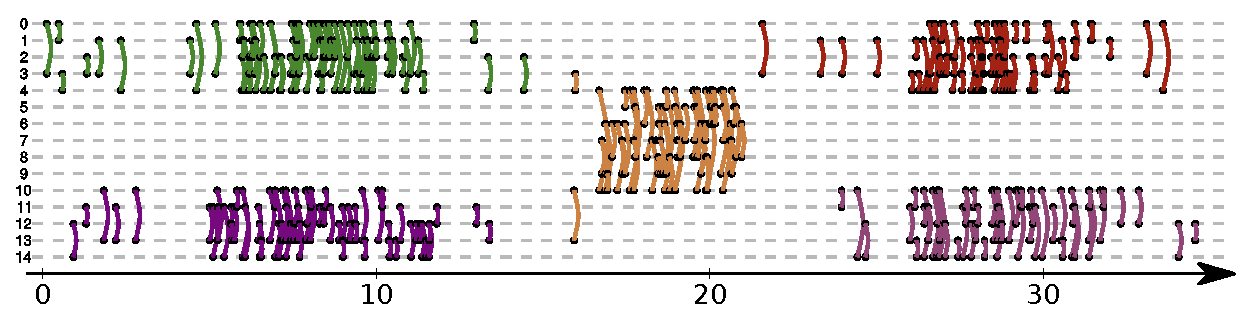
\includegraphics[width=\linewidth]{img/Intro/Dessin_Flot.eps}
            \vspace*{0.7cm}
            \flushleft{Soutenue publiquement le 11 Octobre 2016 devant le jury composé de}\\[2ex]
            \vspace*{0.1cm}
            \flushleft{\begin{tabular}{llll}
                    \emph{Rapporteurs:} &  David \textsc{Chavalarias} & Directeur de recherche, \textsc{CNRS}\\
                     &  Jean-Loup \textsc{Guillaume} & Professeur, Université de la Rochelle\\
                     \emph{Examinateurs:} &  Bertrand \textsc{Jouve} & Directeur de recherche, \textsc{CNRS} \\
                     &  Catherine \textsc{Matias} & Directrice de recherche, \textsc{CNRS} \\
                     &  Gilles \textsc{Tredan} & Chargé de recherche, \textsc{CNRS}\\
                     &  Véronique \textsc{Serfaty} & Responsable scientifique, DGA  \\
                     \emph{Directeurs:} &  Clémence \textsc{Magnien} & Directrice de recherche, \textsc{CNRS}\\
                     &  Matthieu \textsc{Latapy} & Directeur de recherche, \textsc{CNRS}\\
                \end{tabular}
            }
      
 \end{titlepage}
% - - - - - - - fin de la page de garde

%\begin{titlepage}
%\begin{center}
%
%{\scshape\LARGE \univname\par}\vspace{1.5cm} % University name
%\textsc{\Large Doctoral Thesis}\\[0.5cm] % Thesis type
%
%\HRule \\[0.4cm] % Horizontal line
%{\huge \bfseries \hspace*{-0.22cm} \ttitle\par}\vspace{0.4cm} % Thesis title
%\HRule \\[1.5cm] % Horizontal line
% 
%\begin{minipage}[t]{0.4\textwidth}
%\begin{flushleft} \large
%\emph{Auteur:}\\
%\authorname % Author name - remove the \href bracket to remove the link
%\end{flushleft}
%\end{minipage}
%\begin{minipage}[t]{0.4\textwidth}
%\begin{flushright} \large
%\emph{Directeurs:} \\
%\supname % Supervisor name - remove the \href bracket to remove the link  
%\end{flushright}
%\end{minipage}\\[3cm]
%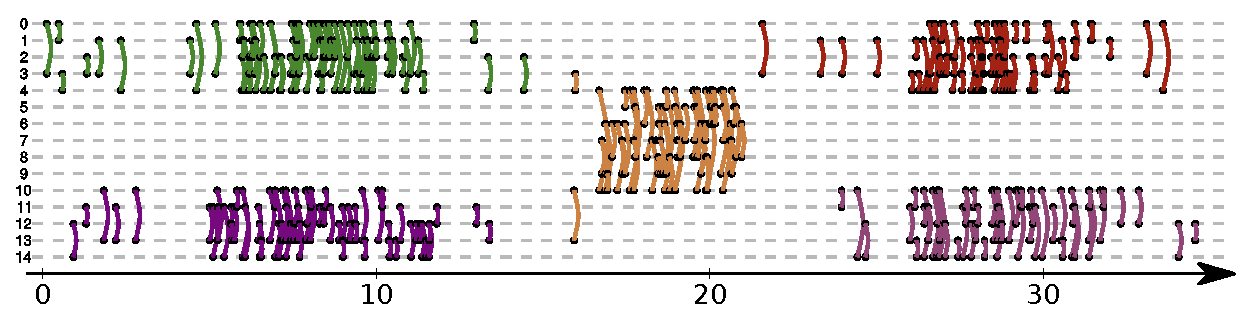
\includegraphics[width=\linewidth]{img/Intro/Dessin_Flot.eps}
%%\includegraphics[width=\linewidth]{img/GroupeDense/GroupExample/Zone_dense.eps}
% 
%\large \textit{A thesis submitted in fulfillment of the requirements\\ for the degree of \degreename}\\[0.3cm] % University requirement text
%\textit{in the}\\[0.4cm]
%\groupname\\\deptname\\[2cm] % Research group name and department name
% 
%{\large \today}\\[4cm] % Date
%%\includegraphics{Logo} % University/department logo - uncomment to place it
% 
%\vfill
%\end{center}
%\end{titlepage}


\begin{acknowledgements}
\addchaptertocentry{Remerciements} % Add the acknowledgements to the table of contents


Je tiens tout d'abord à remercier mes encadrants Clémence et Matthieu qui ont été présent tout au long de ma thèse.
Grâce à eux, j'ai fait mes premiers pas dans le très vaste monde de la recherche.
Il me reste beaucoup à apprendre mais leur encadrement me permet aujourd'hui d'être serein vis-à-vis du chemin encore à venir.

\medskip

Je remercie David Chavalarias et Jean-Loup Guillaume qui ont accepté d'être rapporteur, ainsi que Bertrand Jouve, Catherine Matias, Gilles Tredan et Véronique Serfaty qui ont bien voulu faire parti de mon jury.

\medskip

Tout ce que j'ai réalisé est le fruit de nombreux échanges, scientifiques et humains, avec les membres de l'équipe complex network et je les remercie pour tout ce qu'ils m'ont apportés.
En particuliers, merci à François qui m'a réconcilié avec une partie des probabilités, bien qu'il me reste du travail pour l'autre moitié.
Merci à Lionel et à Tiphaine avec qui j'ai pu discuter science mais également du monde de la recherche en général.
Merci à Aurore qui aura égaillé mon bureau avec de nombreux dessins qui m'ont aidé durant les moments de réflexions intenses.
Je tiens également à mentionner dans mes remerciements Véronique qui a réussi le tour de force de rendre compréhensible et presque agréable les formalités administratives grâce à son efficacité et à sa gentillesse.

\medskip

Je voudrais également remercier mes relecteurs finaux, mon père et Perrine, qui ont eu la lourde tâche de faciliter la lecture de cette thèse.
Le travail a été important mais c'est avec bonne humeur que les touches finales ont été apportées.

\medskip

Alice, nous nous sommes croisé durant la première année de ma thèse et, grâce à toi, elle a été joyeusement entrecoupée de pauses, de jeux, de cookies et de discussions sans aucune mauvaise foi ni cynisme.
J'espère que l'on se retrouvera à de nombreuses autres occasions pour continuer nos débats tout à fait constructifs.

\medskip

Maximilien Danisch, tu aura été mon cobureau pendant deux ans et ce fut un plaisir.
Nous avons à de multiples reprises partagées nos visions du système politique actuel que ce soit lors de petit déjeuners ou à l'escalade.
Tu m'as surtout aidé à garder confiance en mon travail avec tes nombreux encouragements.
Ta motivation et ta détermination m'impressionneront toujours.
Tu a été un vrai partenaire tout au long de cette thèse et je t'en remercie.

\medskip

\`A l'inverse, je souhaite remercier ma famille et mes amis pour m'avoir permis de penser à autre chose qu'à ma thèse et ainsi de garder un rythme de vie sain.
Merci en particuliers à toi Perrine, tu es pour moi une source de joie et de bonheur.

\medskip

Enfin merci à toi, lecteur ou lectrice, de lire ce manuscrit de thèse.
Tu es une des raisons pour laquelle j'ai rédigé ce document.
Le reste du manuscrit n'est sûrement pas aussi divertissant à lire mais peut-être arriverais-je à te partager quelques unes des connaissances acquises durant ma thèse.

\vfill

\hfill Bonne lecture
\end{acknowledgements}


\tableofcontents


\mainmatter % Begin numeric (1,2,3...) page numbering

\pagestyle{thesis} % Return the page headers back to the "thesis" style

%\listoftodos
\adjustmtc

\chapter*{Introduction}
\addstarredchapter{Introduction}

\chapter{État de l'art sur la détection de communautés et les réseaux dynamiques}
\minitoc
\label{chap:etat_art}
Dans cette thèse, nous étudions deux axes de recherches liés aux graphes qui sont orthogonaux.
D'une part, il s'agit de la détection de structures dans les graphes et plus particulièrement de communautés.
Un communauté est un sous-ensemble de n\oe uds de manière à ce qu'ils soient fortement connectés.
Il n'existe cependant aucune définition exact et la notion de communauté fortement connectée dépends du contexte et de la méthode.
Malgré cette définition floue, des structures communautaires ont été trouvées dans de nombreux graphes dans plusieurs domaines tel que le réseaux constitué des région du cerveau \cite{DeReus2014}, le réseau de distribution d'eau \cite{DiNardo2015} et un réseau d'interactions d'animaux \cite{Farine2015}.
Ces notions de communautés et les méthodes de détection sont définies dans la section~\ref{sec:intro_communaute}.\\

D'autre part, il a été observé que la modélisation d'un réseau sous la forme d'un graphe peut poser problème notamment quand le réseau change au cours du temps \cite{Holme2015b}.
D'une part, l'information temporelle est complètement perdue lorsque l'on manipule un graphe.
Par conséquent, certaines structures peuvent devenir indétectable.
Imaginons un graphe représentant les alliances politiques dans un pays.
Si toutes les alliances politiques sont agrégées sur une trop grande durée temporelle, alors une personne politique changeant de parti politique sera faussement considérée comme influente car connectée à plusieurs partis alors qu'elle peut ne plus avoir de contact dans son ancien parti.
Ainsi il n'est plus possible d'observer le glissement des alliances politiques dans ce genre de réseau si l'agrégation temporelle est trop importante~\cite{Mucha2010}.

D'autre part, si on prends en compte le temps, alors il est possible de détecter des structure plus fine que dans le cas statique.
Il devient possible de détecter des instant où l'organisation générale change~\cite{Rosvall2010}, de comprendre à quels sont les instant où une personnes est importante~\cite{Magnien2015}, ou bien de détecter des groupes temporelles~\cite{Cazabet2010}.
Face à ces problèmes plusieurs extensions de la théorie des graphes ont été proposées et elles sont résumées dans la section~\ref{sec:intro_extension_temporelle}.

Mais avant de présenter ces deux axes de recherches, nous revenons dans la section~\ref{[sec:def_graphe]} sur quelques définitions formelles et notation des graphes que nous utilisons dans cette thèse.
\section{Définition dans les graphes}
\label{sec:def_graphe}

Un graphe $G$ est défini par un couple $(V, E)$  où $V$ est une ensemble de n\oe uds et $E$ un ensemble de liens chaque lien est une paire de n\oe uds.
Sauf mention contraire, nous considérons des graphes non-orienté, c'est-à-dire pour toute pair de n\oe uds $u,v \in V$ les liens $(u,v)$ et $(v,u)$ sont équivalents.
Nous considérons également uniquement des liens non-pondérés, c'est-à-dire qu'un lien est soit présent soit absent.
Enfin, nous ne considérons que des graphes simples, c'est-à-dire qu'il n'existe au maximum qu'un seul lien entre deux n\oe uds.
Ceci est en opposition avec les graphes multiples où il peut exister plusieurs liens entre deux n\oe uds.

Par convention, nous définissons $n=|V|$ le nombre de n\oe uds et $m=|E|$ le nombre de liens.
Il est possible de représenter un graphe $G$ par une matrice carré $A$ de taille $n$ où la case $A_{i,j} \ \forall i,j \in \mathbb{N}^+ \leq n$ est égale à $1$ si un lien relie les n\oe uds $i$ et $j$ et $0$ sinon.


Le degré d'un n\oe ud $i$, noté $d_i$, est égale au nombre de liens reliés à $i$: $d_u = \sum_{j\leq n} A_{i,j}$.

Une chaine ou chemin entre deux n\oe uds dans un graphe est une suite de liens $((u_1,v_1),...,(u_k,v_k))$ de tel sorte que $v_{i}=u_{i+1} \ \forall i \in [0,k-1]$.
Les n\oe uds d'un graphe sont dit connexe s'il existe un chemin entre toute les pairs de n\oe uds.
Une composante connexe est un ensemble de n\oe uds $V'\subseteq V$ qui est connexe et maximal, c'est-à-dire qu'il n'est pas possible d'ajouter un n\oe ud dans $V'$ tel que $V'$ soit toujours connexe.

La densité, $d(G)$ dans un graphe est la probabilité que deux n\oe uds soient reliés par un lien: $d(G)=\dfrac{2m}{n(n-1)}$.

Le graphe connexe le moins dense est un arbre et est constitué de $n-1$ liens pour $n$ n\oe uds.
Le graphe le plus dense est appelé un graphe complet ou un clique et est composé de $\dfrac{n(n-1)}{2}$ pour $n$ n\oe uds.


\subsection{Définition de structure dans un graphe}

 partition, couverture,

\subsubsection{Comparaison}
ARI, NMI \cite{Danon2005}, futur nmi\cite{Zhang2015}, F1-score, Omega index \cite{Porumbel2011}


\section{Communauté dans les graphes}
\label{sec:intro_communaute}

Ce champs de recherche est très vaste et il est illusoire de vouloir énumérer les méthodes existantes dans ce domaine car les caractéristiques voulues d'une communauté peuvent varier selon le contexte~\cite{Coscia2011,Leskovec2008,Yang2015,Jeub2015}.
Il y a tout de même deux grandes catégories qui permettent de séparer les méthodes existantes.
Dans ces deux catégories, les méthodes existantes cherchent à capturer 
des communautés fortement connectées mais elles différent sur ce qu'elles capturent comme structures communautaires.
Les communautés d'une structure communautaire peuvent être disjointes, c'est-à-dire que deux communautés n'ont aucun n\oe uds en commun, ou alors recouvrantes, c'est-à-dire que deux communautés peuvent avoir plusieurs n\oe uds en commun.
Dans le premier cas, on parle de partition des n\oe uds et dans le second on parle de couverture ou partitions chevauchantes de n\oe uds.
Dans ces deux cas, il y a également une contrainte sur le fait que tout les n\oe uds doivent appartenir à au moins une communauté.
Ces deux structures correspondent à deux visions possibles de l'organisation d'un graphe et du réseau sous-jacent.
Nous présentons ces deux catégories dans les sous-sections suivantes.
Il existe également une troisième catégorie qui est la détection de partition de liens qui est un problème à part et qui est présentée dans le chapitre~\ref{chap:Expected_Node}.

\subsection{Parititons de n\oe uds}
Afin de mieux comprendre ce que peux capturer une parition de n\oe uds, il est plus facile de partir d'un exemple.
Dans l'étude de Stehlé~\emph{et al.}~\cite{Stehle2011}, des enfants d'une école primaire ont eu pendant 2 jours des capteurs enregistrant lorsque deux enfants sont à une distance de moins de 1m50 l'un de l'autre.
Ce dispositif permet de mesurer les interactions entre élèves et de construire le graphe des relations entre élève à l'école.
Une illustration du graphe obtenu est visible dans la figure~\ref{fig:ecole_primaire}.
La classe de chaque élève est également connue.
Comme chaque élève appartient à une et une seule classe, les classes forment une partition des élèves.
Cette partition est une bonne structure communautaire car on remarque que les élèves d'une même classe parle beaucoup entre eux mais ils parlent peu entre élèves de classes différentes.
Cela se remarque particulièrement bien pour la classe 3A.
Il existe beaucoup de liens entre les élèves de la classe 3A et aucun entre eux et les élèves de la classe 5A par exemple.

\begin{figure}
\centering
\includegraphics[width=0.7\linewidth]{img/Intro/ecole_primaire}
\caption{Graphe de contact des enfant d'une école primaire. L'épaisseur du lien représente la durée de communication entre deux élèves. La couleur représente la classe de chaque élèves. Les professeurs sont en gris.\protect\footnotemark}
\label{fig:ecole_primaire}
\end{figure}
\footnotetext{Image provenant de \url{http://journals.plos.org/plosone/article?id=10.1371/journal.pone.0023176}.}

Afin de capturer des partitions de n\oe uds, beaucoup de méthodes existent.
Il y a d'ailleurs régulièrement des état de l'art qui sont publiés~\cite{Fortunato2010,Plantie2013a, Malliaros2013a, Harenberg2014a}.
Afin d'aider le lecteur, nous détaillons ici quelques unes des méthodes les plus utilisées.

\subsubsection{Méthodes utilisant un modèle pour la comparaison}

Comme une communauté est souvent définie comme devant être très connectée, le problème est de trouver une fonction capable d'évaluer la connexité d'une communauté.
Pour ce faire, deux \emph{ingrédients} sont nécessaires.
Tout d'abord, il faut définir une métrique qui mesure la connexité, \emph{e.g.} le nombre de liens dans un groupe.
Puis, il est nécessaire de définir comment utiliser la métrique pour considérer qu'un groupe est très connecté.
Il est possible d'utiliser une métrique en la normalisant par ses bornes minimum et maximum.
Avec cette métrique normalisée entre $0$ et $1$, un groupe est considéré comme très connectés si son évaluation est supérieur à un certain seuil.
Cette approche n'est cependant pas adaptée pour la recherche de communauté car elle ne tiens pas compte de la structure du graphe\,\footnote{C'est plus approprié dans la recherche des groupes les plus denses~\cite{Balalau2015}.}.
Prenons l'exemple du graphe constitué d'une clique et du nombre de liens comme métrique.
Le nombre de lien d'un groupe est normalisé par le nombre minimum de liens, $0$, et par le nombre de maximum de liens qui est obtenu par une clique.
Dans ce graphe, tout groupe de n\oe uds est également une clique et par conséquent tout groupe de n\oe uds a un évaluation parfaite de $1$.
Chaque groupe serait donc une très bonne communauté selon cette évaluation.
Or, le graphe constitué d'une unique clique ne possède pas de structure communautaire contrairement au graphe dans la figure~\ref{fig:ecole_primaire}.
Il est donc nécessaire de trouver une autre approche.

Plutôt que de normaliser une métrique par ces valeurs minimum et maximum, il est intéressant de considérer l 'écart à une valeur moyenne.
L'idée est la suivante: si le graphe n'avait pas de structure communautaire qu'elle serait la valeur attendue de la métrique considérée?
Le problème est alors de définir des graphes qui n'ont pas de structures communautaires.
L'ensemble des graphes similaires définit alors un \emph{modèle nul}.
Détecter des communautés se traduit alors en trouver des groupes qui s'éloignent du modèle nul considéré où il n'existe pas de communauté.
Ce changement est astucieux car il est relativement aisé de définir des graphes n'ayant pas de structure.
Il suffit de créer des graphes complètement aléatoires~\cite{Erdos1959} où les liens du graphes sont tirés de manière uniforme.
Afin que les graphes aléatoires puissent être comparable au graphe initiale, des contraintes sont généralement ajoutées et donnent lieu à différent modèle nul.
Le premier modèle nul de graphe est celui de Erdös-Rényi~\cite{Erdos1959} où le nombre de liens et le nombre de n\oe uds des graphes aléatoires doivent être les mêmes que dans le graphe initial.
Un autre modèle très couramment utilisé est le modèle de configuration~\cite{Bender1978a}.
Dans ce modèle, la distribution des degrés est également fixe.
Le modèle est de configuration est souvent utilisé car il a été souvent observé que les graphes provenant de données réelles ont une distribution des degrés très éloignés d'une distribution uniforme.
C'est pourquoi l'ajout de la contrainte sur les degrés permet de considérer des graphes dans le modèle nul plus similaire au graphe initiale. 
Ils existent bien évidement d'autres modèles possibles considérant d'autres contraintes~\cite{Newman2009}.

\paragraph{Modularité}
La modularité~\cite{Newman2004} est une fonction qui associe a chaque partition de n\oe uds une valeur de qualité entre $-1$ et $1$.
Plus la valeur de modularité d'une partition est élevée, plus la partition est censée capturer une structure communautaire.
La modularité est définie de la manière suivante pour une partition $\mathcal{C}$:

\begin{equation}
Q(\mathcal{C}) = \dfrac{1}{2M}\sum_{i,j \in V} \left(A_{ij} - \dfrac{d_id_j}{2M}\right)\ \delta_{C(i)=C(j)} \ .
\end{equation}
Il s'agit pour deux n\oe uds d'une même communauté de comparer la présence ou absence d'un lien,$A_{ij}$, à la probabilité que ces des n\oe uds soient reliés dans le modèle de configuration, $\dfrac{d_id_j}{2M}$.
L'idée sous-jacente est que les n\oe uds d'une communauté devraient partager plus de liens qu'espéré dans le modèle de configuration.
De très nombreux travaux ont par la suite étudié les caractéristiques de la modularité et son optimisation.
Tout d'abords, il a été montré que l'optimisation de la modularité est un problème NB-Complet~\cite{Brandes2007}.
Il est donc nécessaire de recourir à des heuristiques afin de trouver rapidement une partition proche de l'optimum
Parmi l'ensemble des algorithmes existant, l'algorithme de Louvain~\cite{Blondel2008a} est un des plus rapide.
Il existe également des variantes de cet algorithme~\cite{Huang2015,Traag2015a}.
D'autres travaux se sont attachés à l'étude de la modularité.
Il a été montré que la modularité souffre du problème de \emph{résolution limite}~\cite{Fortunato2007,Lancichinetti2011} car le modèle de configuration présuppose une répartition uniforme des tailles des communautés.
Il a par ailleurs été montré que la modularité n'offre pas de maximum clair et que beaucoup de partitions différentes ont des évaluations proches~\cite{Good2010}.
Pour répondre à ces problèmes, il existe des variantes~\cite{Reichardt2006,Delvenne2010}.

\paragraph{Surprise}
La fonction Surprise~\cite{Aldecoa2011,Traag2015b} est une autre fonction de qualité qui se base quant a elle sur le modèle de Erdös-Rényi pour évaluer la surprise d'observer un groupe de n\oe uds relié par $l$ liens.

\paragraph{Stochastic Block Model}
Nous avons définis précédemment la notion de modèle nul permettant de se comparer à l'absence de communautés.
Il est également possible de modéliser une structure communautaire puis de vérifier \emph{a posteriori} si ce modèle pourrait être à l'origine du graphe observé.
Le problème de détection de communauté est alors un problème d'inférence qui est traité avec des outils statistiques tel que le \emph{stochastic block model} (SBM)~\cite{Holland1983a,Nowicki2001}.
L'idée derrière le SBM est la suivante: la probabilité que deux n\oe uds soient reliés dépend uniquement de leur groupe respectif.
Si le graphe a une structure communautaire, alors deux n\oe uds d'une même communauté devraient avoir une forte chance d'être connecté.
\`A l'inverse, deux n\oe uds de deux communauté différentes devraient avoir une probabilité assez faible d'être connecté.
Le SBM est défini par de nombreux paramètres: le nombre de groupe, l'assignation d'un groupe à chaque n\oe ud et les probabilités d'interactions entre les groupes.
Avec un jeu de paramètres donné, il est alors possible de calculer la vraisemblance que ce jeu de paramètre soit à l'origine du graphe.
Trouver une partition de n\oe uds dans ce contexte est alors équivalent à trouver le jeu de paramètre qui est le plus vraisemblablement à l'origine du graphe.

Dans le SBM, tout les n\oe uds sont considérés comme équivalents en particulier vis-a-vis du degré ce qui n'est pas le cas dans beaucoup de graphes provenant de données réelles.
C'est pourquoi une version tenant compte du degré des n\oe uds a été proposée: le Degree-correcte Stochastic Block Model (DBSM)~\cite{Karrer2011}.
Enfin d'après de récents travaux\cite{Newman2016}, il semblerait que le DSBM et l'optimisation de la modularité soient liés.

\subsubsection{Méthodes utilisant des marches aléatoires}
Il existe de nombreuses autres approches que celles utilisant un modèle nul ou un modèle générateur.
Notamment, il y a des méthodes utilisant les marches aléatoires \cite{Pons2005,Rosvall2008}.
Ces méthodes tirent partis du fait que si une communauté est densément connectée alors un marcheur aléatoire devrait y rester assez longtemps.
En particulier, la méthode Infomap~\cite{Rosvall2008} repose sur une idée très élégante; une partition de n\oe uds est une carte du graphe et, en ce sens, elle doit aider sa lecture.
Une carte est efficace si elle permet de mieux comprendre l'objet d'étude en réduisant sa complexité.
Dans une carte d'un pays, les départements découpent l'espace en zones compactes et la plupart du temps la majorité des routes se retrouvent à l'intérieur des départements.
Ainsi un voyageur se déplaçant aléatoirement sur les routes a peu de chance de sortir d'un département.
Pour décrire, \emph{a posteriori}, l'ensemble des routes prises par ce voyageur, il suffit alors de donner le département initiale puis la liste des routes empruntées.
Il n'est pas nécessaire de répéter le département à chaque fois si le voyageur n'en est pas sortit.
En ce sens, la découpe d'un pays en département permet de réduire la complexité du voyage.
Il s'agit donc d'un problème lié à la théorie de l'information et de sa compression.
De manière similaire, Rosval~\emph{et al.} utilise des marcheurs aléatoires se déplaçant sur les n\oe uds du graphe et les communautés forment des zones du graphe.
Si les communautés sont bien formées et que les marcheurs aléatoires restent bloqués à l'intérieur, alors la description de leur marche aléatoire sera courte.
La longueur de cette description devient alors la signature de la partition et plus la signature est courte, meilleur la partition est.

La méthode a également été étudiée pour voir si elle souffre de \emph{résolution limite} comme la modularité~\cite{Kawamoto2015}.
Il semble que cet effet existe également dans Infomap mais qu'il soit beaucoup moins prononcé.

\paragraph{Autres méthodes}
Il existe bien d'autres méthodes pour détecter des communautés en tant que partition de n\oe uds.
Il y a les méthodes spectrales~\cite{Donetti2004,Mitrovic2009} qui se base sur les vecteurs propres de la représentation d'un graphe sous la forme d'une matrice.
De manière moins formelle, les méthodes sont des algorithme de propagations de labels (LPA)~\cite{Raghavan2007a,Li2014c}.
Dans ces méthodes, chaque n\oe uds a initialement un label puis à chaque itération chaque n\oe ud prend comme label un des label de ses voisins.
En général, un n\oe ud prend comme label celui qui est le plus présent parmi ses voisins.
Au bout d'un certain nombre d'itération ou l'équilibre, il ne reste que beaucoup moins de labels qui représentent les communautés.


\resume{Il existe de très nombreuses méthodes pour la détection de communautés en tant que partition de n\oe uds. Ils semblent que les méthodes d'optimisation de \textbf{modularité}, la méthode \textbf{infomap} et  les \textbf{Stochastic Block Model} soient les plus utilisées dans la littérature.}

\subsection{Couverture de n\oe uds}
\label{subsec:cover}
Jusqu'à maintenant nous avons considérons les communautés comme des partition de n\oe uds.
Or, les partitions sont très restrictives et ne peuvent pas capturer toutes les situations possibles.
Reprenons l'exemple d'un graphe reflétant des interactions de personnes comme dans la section~\ref{sec:intro_communaute}.
Ils existent des communautés qui sont disjointes comme le travail et la famille mais bien souvent des personnes appartenant à plusieurs groupes, voire l'exemple dans la figure~\ref{fig:ex_overlap_communaute}.
Ainsi le groupe de personnes faisant du sport ensemble et le groupe des personnes travaillant ensemble peuvent ne pas être disjoint.
Si tel est le cas, alors il n'est plus possible de représenter des communautés avec une partition.
Il est nécessaire de manipuler une couverture de n\oe uds.
Ainsi dans l'exemple dans la figure~\ref{fig:ex_overlap_communaute}, les n\oe uds rouges devraient appartenir deux groupes au lieu d'un seul.

\begin{figure}
	\centering
	\includegraphics[width=0.31\linewidth]{img/Intro/Illustration_of_overlapping_communities.jpg}
	\caption{Exemple graphe avec une structure communautaire chevauchante représenté par les couleurs\,\protect\footnotemark.}
	\label{fig:ex_overlap_communaute}
\end{figure}
\footnotetext{Image provenant de \url{https://en.wikipedia.org/wiki/Clique_percolation_method}.}

Une fois encore, la littérature est très vaste dans ce domaine et nous ne ferons pas une liste exhaustive des méthodes existantes.
Pour une liste plus exhaustive, il existe de nombreux état-de-l'art dans le domaine~\cite{Danisch2012, Kanawati2014, Xie2013,Bandyopadhyay2015, Hric2014a}.

Une des premières méthodes de détection de couverture de n\oe uds est la \emph{Clique Percolation Method} (CPM)~\cite{Palla2005}.
L'algorithme CPM repose sur le principe de transitivité qui serait à l'origine des communautés: si $i$ et $j$ sont reliés par un lien alors le n\oe ud $k$ qui est déjà relié à $i$ a une forte chance d'être également connecté à $k$.
Il s'agit de la formalisation du proverbe "Les amis de mes amis sont mes amis".
Si ce principe est réellement à l'origine des communautés, alors elles doivent être composées de plusieurs cliques.
C'est pourquoi CPM cherche l'ensemble des cliques d'une taille $k$ donnée, en générale $k<10$ pour des raisons de coût de calcul, puis fusionne toutes les cliques qui partagent suffisamment de n\oe uds, en générale $k-1$. 
Comme cette méthode est relativement couteuse, Kumpula \emph{et al.}~\cite{Kumpula2008} ont repris le même mécanisme en optimisant le mode de calcul.

\subsubsection{Extension de méthodes existantes}

La majorité des méthodes existantes pour les partitions ont été adaptées pour manipuler les couvertures de n\oe uds.
Il existe plusieurs extensions de la modularité~\cite{Shen2009,Nicosia2009}.
Cependant ces extensions ne reposent plus sur un modèle nul car elles introduisent des termes de normalisations.
Par conséquent, ces extensions sont beaucoup moins utilisées que la modularité initiale.

\paragraph{Stochastic Block Model}
En revanche, le SBM s'adapte très bien aux couvertures de n\oe uds.
Une extension du SBM est le Mix-Membership Stochastic Block Model (MMSBM)\cite{Airoldi2008} qui permet à un n\oe uds d'avoir plusieurs groupes.
Dans~\cite{Gopalan2013a}, les auteurs utilisent la même méthodes mais en échantillonnant le graphe initiale afin de réduire le cout de calcul.
Il existe d'autres méthodes à base de modèle génératif~\cite{Ball2011,Yang2013}.
Ces méthodes se basent sur des graphe d'affiliation\cite{BreigerRonald1974}.
Un graphe d'affiliation est un graphe biparti entre les n\oe uds d'une part et les communautés de l'autre part.
Dans la méthode de Ball\emph{et al.}, ce graphe d'affiliation est pondéré et la pondération représente la propension d'un n\oe uds à créer des liens dans un groupe donné tant dis que dans Yang\emph{et al.} il s'agit du facteur d'appartenance du n\oe uds au groupe.
Une fois le graphe d'affiliation définit, il est nécessaire de savoir recréer la matrice d'adjacence et, en ce sens, ces méthodes se rapprochent des méthodes de factorisation non négative de matrices~\cite{Lee1999}.
Le but de la factorisation non-négative d'une matrice donnée est d'être capable de trouver deux matrices dont les entrées sont non-négatives tel que leur combinaison permettre de retrouver la matrice initiale.

Jusque récemment ce genre de technique généralisant le SBM ne pouvaient s'appliquer qu'à des graphes relativement petit.
il semble cependant que les méthodes récentes~\cite{Gopalan2013a, Yang2013} arrivent à traiter des graphes ayant énormément de liens, de l'ordre $10^{12}$ liens.



\paragraph{Propagation de label}
Des méthodes ont étendus la propagation de label aux couvertures de n\oe uds~\cite{Gregory2010,Xie2011}.
Le principal changement est qu'un n\oe ud ne stocke plus un unique label mais soit plusieurs labels soit des fréquences d'apparition de label.
Ainsi à la fin de l'algorithme, il suffit de choisir les labels les plus fréquents.
Cependant ce mécanisme de propagation change radicalement de l'idée initiale.
En effet, la diffusion d'un label n'est plus directement contrainte par la diffusion des autres labels.
Dans cette nouvelle configuration, il est possible qu'un label soit présent dans tout les n\oe uds.
De plus selon les auteurs de ces méthodes, des communautés non connexes peuvent apparaître ce qui nécessite l’ajout d’un mécanisme de post-processing.


\paragraph{Infomap}
Il s'agit surement de la méthode étant le moins "déformé" avec le SBM par l'adaptation aux partitions chevauchantes.
En effet, il suffit de relâcher la contrainte sur le fait qu'un n\oe ud n'appartienne qu'à un seul groupe.
Il est toujours possible de décrire un trajet par un nom de groupe puis une liste de n\oe uds visités dans le même groupe.
Ainsi, la notion de longueur de description est toujours valide même dans contexte.
Ce travail d'extension a été fait par Esquivel\emph{et al.}~\cite{Esquivel2011}.

\subsubsection{Méthodes utilisant des fonctions de qualité locales}
On a vu avec la modularité qu'il est assez difficile de définir une fonction de qualité évaluant une couverture de n\oe uds en fonctions des caractéristiques des groupes.
En revanche, les LPA tirent partis de l'information locale pour créer des groupes locales mais ne permettent pas leur évaluation.
L'idée est en quelque sorte mélanger ces deux aspects.
Il s'agit d'algorithmes qui initialement considèrent de très petites communautés puis essayent de les étendre itérativement en ajoutant des n\oe uds.
Afin de ne s'étendre un groupe indéfiniment comme cela peut être le cas avec les LPA, un ajout n'est fait que s'il améliore une fonction de qualité locale.
Ainsi dans ce type d'algorithme, il y a principalement deux critères important:
le choix des communautés initiales et le critère d'évaluation.
Dans la majorité des cas, chaque n\oe ud constitue une communauté. 
OSLOM\cite{Lancichinetti2011a} diffère de cette situation car OSLOM utilise comme point de départ une partition trouvée par l'algorithme de Louvain ou par infomap.

Les fonctions de qualité applicable sont très nombreuses et nous ne mentionneront que trois.
Tout d'abord, il est possible d'utiliser le degré relatif~\cite{Luo2008} d'un groupe comme critère.
Il s'agit du ratio entre le nombre de $l_{in}$ liens internes à un groupe de n\oe uds et du nombre de liens totale $l_{in}+l_{out}$:$ \dfrac{l_{in}}{l_{in}+l_{out}}$.
En effet, plus le degré relatif est élevé, plus le groupe est dense comparé à son voisinage et plus il a de forte chance d'être une bonne communauté. 
Cette formulation est assez proche de la conductance ou coupe normalisée\cite{Shi2000}:
\begin{equation}
\phi =\dfrac{l_{out}}{\min \left( 2(l_{in}+l_{out}),m-2(l_{in}-l_{out}) \right) }
\end{equation}

Ces deux notions se rapportent à la notion de densité vis-à-vis de leur voisinage.
Il également possible d'évaluer une communauté locale par rapport aux nombre de triangles présents de la communauté.
C'est ce que mesure la cohesion~\cite{Friggeri2011} pour un groupe de taille $k$: 
\begin{equation}
cohesion=\dfrac{\Delta_3}{ {k \choose 3} } \times \frac{\Delta_3}{\Delta_3+\Delta_2},
\end{equation}
où $\Delta_3$ est le nombre de triangle dont les 3 n\oe uds sont à l'intérieur du groupe et $\Delta_2$ est le nombre de triangle dont unqiement 2 n\oe uds sont à l'intérieur du groupe.

Différentes méthodes d'initialisation ainsi que fonctions de qualité sont déaillées dans l'article de Kanawati~\cite{Kanawati2014}.
Ces méthodes semblent très prometteuses car elles permettent de traiter efficacement de très grand graphe tout comme les LPA mais elles profitent des fonctions de qualité locales qui permettent d'une certaines manières d'évaluer le résultat obtenus.


\resume{
La littérature sur la détection de couverture de n\oe ud est encore très récente.
Il est donc délicat de commencer à tirer des conclusions.
Cependant, il semble que les extensions de la modularité ne soient pas réellement capable de trouver des couvertures de n\oe uds.
En plus d'infomap, c'est surtout les méthodes utilisant des modèles génératifs et celles utilisant des fonctions de qualité locales qui semblent les plus à même de capturer des couvertures de n\oe uds pertinentes.
Bien que souvent limité à de petit exemple, les modèles génératifs semblent maintenant capable de traiter des graphes de tailles importantes.
Les méthodes utilisant des fonctions de qualité locales sont quant à elle très rapide mais le choix de la fonction de qualité semble encore délicat.
}




%benchmark \cite{Lancichinetti2008,Lancichinetti2009b}

\section{Extension temporelle des graphes}
\label{sec:intro_extension_temporelle}

\cite{Hartmann2014}

application:
Diffusions \cite{Backlund2014, Gauvin2015} \cite{Karimi2013,Holme2014a,Horvath2014,Karsai2011,Kivela2012,Lambiotte2013,Lee2012,Perotti2014,Rocha2011,Scholtes2014,Scholtes2013}temporal network \cite{Jo2014} impact inter event time
Face-to-face interaction: \cite{Barrat2013,Asur2009}
Communauté TVG: \cite{Bassett2013,Bazzi2016}
Réseau de transport: \cite{Gallotti2015} multilayer
\subsection{snapshot}
multylayer \cite{Mucha2010,Kivela2014,Peixoto2015c},mathemical source\cite{DeDomenico2013}, survey générale (génération, percolation, diffusion) \cite{Boccaletti2014}

snap\cite{Asur2009,Bassett2013,Bazzi2014} + fenetre glissante
\cite{de2016detection,Rosvall2010} change point snap

effet time window \cite{Krings2012,Ribeiro2013} (ribeiro effet sur les random walk)

centralité de lien \cite{Takaguchi2012}

Communauté:
\cite{Sun2007} graphescope
\cite{Lin2008} facenet
\cite{DeDomenico2014} info map sur du multi layer
\cite{Chakrabarti2006,Chen2013} current + stabilité
Multylayer SBM\cite{Stanley2015} \cite{Corneli2016} SBM sur chaque tranche. proche\cite{Matias2015}
\cite{Gauvin2014}
\cite{Guo2014}
\cite{Hopcroft2004}
\cite{Kalavathi2015}
temps intrinsèque.
\cite{Albano2014}

Génération de: \cite{Granell2015, Karsai2014,Perra2012}

\subsection{TVG/Evolving}
\cite{Casteigts2011,Wehmuth2014}
\cite{Figueiredo2012} random walk.
\cite{Cazabet2010} conductance sur TVG
Suivi dans les snapshot de la force d'une communauté: \cite{Du2015}
\cite{Caceres2013} time scale on temporal networks 
\cite{Cordeiro2016} évolution modularité
\cite{Epasto2015} le plus dense à un instant
\cite{Sun2014}

\subsection{Flots de liens}
\cite{Holme2013a,Holme2015b,Holme2015} plein d'étude possible
Formalisation algébric \cite{Batagelj2015}.
bursty \cite{Karsai2012a,Karsai2011,Moinet2015,Stehle2010} inter event time \cite{Kivela2014a}, \cite{Malmgren2008,Malmgren2009} heavy tail, \cite{Rocha2013}

motif \cite{Kovanen2011a,Kovanen2013}.
Le formalisme de flot de liens est défini plus en profondeur dans le chapitre~\ref{chap:def_flot}.
randomwalk\cite{Starnini2012b}

\cite{Gaumont2016}
centralité \cite{Costa2015,Kim2012, Pfitzner2013a, Praprotnik2015,Scholtes2015,Takaguchi2016}
densité \cite{Viard2014a}

generateur \cite{Starnini2013,Vestergaard2014}


\chapter{État de l'art sur la détection de communautés et les réseaux dynamiques}
\minitoc
\label{chap:etat_art}
Dans cette thèse, nous étudions deux axes de recherches liés aux graphes qui sont orthogonaux.
Mais avant de présenter ces deux axes de recherches dans les sections~\ref{sec:intro_communaute} et \ref{sec:intro_extension_temporelle}, nous revenons dans la section~\ref{sec:def_graphe} sur quelques définitions et notations utiles pour manipuler des graphes.

Le premier axe de recherche est la détection de structures dans les graphes et plus particulièrement de communautés.
Une communauté est une partie du graphe tel qu'il existe beaucoup de liens à l'intérieur de la communauté et moins avec le reste du graphe.
Il n'existe cependant aucune définition unique et exacte d'une communauté.
La notion de communauté dépend du contexte et de la méthode.
Malgré cette définition floue, des structures communautaires ont été trouvées dans de nombreux graphes dans plusieurs domaines tel que le réseau constitué des régions du cerveau \cite{DeReus2014}, un réseau de distribution d'eau \cite{DiNardo2015} et un réseau d'interactions d'animaux \cite{Farine2015}.
Ces notions de communautés et les méthodes de détection sont définies dans la section~\ref{sec:intro_communaute}.

Le second axe de recherche est la prise en compte du temps dans la théorie des graphes.
La première approche fût de complètement ignorer l'information temporelle et de considérer que tout les liens apparaissent en même temps; on parle alors de graphe agrégé.
Cependant, la modélisation d'un réseau sous la forme d'un graphe agrégé manque de pertinence, lorsque le réseau change trop au cours du temps~\cite{Holme2015b}.
Si tel est le cas, certaines structures présentes dans le graphe peuvent n'être que des artefacts de l'agrégation temporelle.
Imaginons par exemple un graphe représentant les alliances politiques dans un pays sur une longue période.
Si toutes les alliances politiques sont agrégées, alors les personnes changeant de parti politique seront faussement considérées comme influentes car connectées à plusieurs partis alors qu'elles peuvent ne plus avoir de contact dans leur ancien parti.
Ainsi, il n'est plus possible d'observer la répartition des alliances politiques dans ce genre de réseau si l'agrégation temporelle est trop importante~\cite{Mucha2010}.

Si on prend en compte le temps, alors il est possible de détecter des structures plus fines que dans le cas statique.
En effet, il devient possible de détecter des instants où l'organisation générale change~\cite{Rosvall2010}, de comprendre quels sont les instants où un n\oe ud est important~\cite{Magnien2015,Costa2015,Takaguchi2016}, ou bien de détecter des groupes temporels~\cite{Cazabet2010}.
Pour ce faire, plusieurs extensions de la théorie des graphes ont été proposées et elles sont présentées dans la section~\ref{sec:intro_extension_temporelle}.


\section{Définition dans les graphes}
\label{sec:def_graphe}

Un graphe $G$ est défini par un couple $(V, E)$  où $V$ est un ensemble de n\oe uds et $E \subseteq V \times V$ est un ensemble de liens; chaque lien étant une paire de n\oe uds.
Sauf mention contraire, nous considérons des graphes non-orientés, c'est-à-dire pour toute paire de n\oe uds $u,v \in V$, les liens $(u,v)$ et $(v,u)$ sont équivalents.
Nous considérons également uniquement des liens non-pondérés, c'est-à-dire qu'un lien est soit présent soit absent.
Enfin, nous ne considérons que des graphes simples, c'est-à-dire qu'il n'existe au maximum qu'un seul lien entre deux n\oe uds et aucun lien de la forme $(u,u)$.
Ceci est en opposition avec les graphes multiples où il peut exister plusieurs liens entre deux n\oe uds.

Par convention, nous notons $n=|V|$ le nombre de n\oe uds et $m=|E|$ le nombre de liens.
On suppose en général que $V=\{1, ..., n\}$.
Il est possible de représenter un graphe $G$ par une matrice carrée $A$ de taille $n$ où l'élément $A_{i,j} \ \forall i,j \in V$ est égale à $1$ si un lien relie les n\oe uds $i$ et $j$ et $0$ sinon.
Avec ces notations, nous définissons les notions suivantes:
\begin{description}
\item[Degré] Le degré d'un n\oe ud $i$, noté $d_i$, est égal au nombre de liens reliés à $i$: $d_i = \sum_{j \in V} A_{i,j}$;
\item[Densité] La densité, $\delta(G)$ d'un graphe est la probabilité que deux n\oe uds pris au hasard soient reliés par un lien: $\delta(G)=\dfrac{2m}{n(n-1)}$;
\item[Degré moyen] Le degré moyen $\tilde{\delta}(G)$ est égal à : $\tilde{\delta}(G)=\dfrac{2m}{n}$;
\item[Chemin] Un chemin dans un graphe est une suite de liens $((u_1,v_1),...,(u_k,v_k))$ de telle sorte que $v_{i}=u_{i+1} \ \forall i \in [1,k-1]$;
\item[Graphe connexe] Les n\oe uds d'un graphe sont dit connexes s'il existe un chemin entre toutes les paires de n\oe uds du graphe;
\item[Composante Connexe] Une composante connexe est un ensemble de n\oe uds $V'\subseteq V$ qui est connexe et maximal, c'est-à-dire qu'il n'est pas possible d'ajouter un n\oe ud dans $V'$ tel que $V'$ soit connexe;
\item[Arbre] Un arbre est le graphe connexe le moins dense et il est constitué de $n-1$ liens pour $n$ n\oe uds;
\item[Clique] Une clique, aussi appelée graphe complet, est le graphe le plus dense et elle est composée de $\dfrac{n(n-1)}{2}$ liens pour $n$ n\oe uds;
\item[Sous-graphe] Un graphe $G'=(V',E')$ est un sous-graphe de $G$ si et seulement si $V' \subseteq V$ et $E' \subseteq E$;
\item[Graphe induit] Le graphe induit par un ensemble de n\oe uds $V' \subseteq V$ est défini par $V'$ et $E'= E \cap V' \times V'$.  
\end{description}



\subsection{Groupes, partitions et couvertures}
En plus des n\oe uds et des liens, nous manipulons également des ensembles de liens et des ensembles de n\oe uds.
Par convention, notons $X \subseteq V$ un ensemble de n\oe uds et $Y \subseteq E$ un ensemble de liens.
Nous listons les notations utilisées dans le tableau~\ref{tab:notation_groupe_noeuds}.


\begin{table}
  \centering
    \begin{tabular}{|c|c|}
     \hline
    \rule[-1ex]{0pt}{4ex} Notation & Définition \\
  \hline
		\hline
		\rule[-1ex]{0pt}{4ex}$V(Y)=\{u,\ \exists (u,v) \in Y \}$ & n\oe uds induits par les liens de $Y$\\
		\hline
        \rule[-1ex]{0pt}{4ex}$n_X=|X|$ & nombre de n\oe uds dans $X$\\
        \hline
        \rule[-1ex]{0pt}{4ex} $l_{in}(X)=|E \cap (X \times X)|$ & nombre de liens entre les n\oe uds de $X$\\
        \hline
        \rule[-1ex]{0pt}{4ex} $l_{out}(X)=|E \cap (X \times V \setminus X)|$ & nombre de liens entre les n\oe uds de $X$ et de $V \setminus X$ \\
        \hline
        \rule[-1ex]{0pt}{4ex} $l(X)=l_{in}(X)+l_{out}(X)$ & nombre de liens reliés aux n\oe uds de $X$\\
        \hline
        \rule[-1ex]{0pt}{4ex} $d_{in}(u,X)=|\{(u,v) \in E,\ v \in X\}|$ & nombre de liens que partagent $u$ avec $X$ \\
        \hline
        \rule[-1ex]{0pt}{4ex} $d_{in}(X)=\sum_{u \in X} d_{in}(u,X)=2l_{in}(X)$ & somme des degrés internes des n\oe uds dans $X$ \\
        \hline
        \rule[-1ex]{0pt}{4ex} $d_{out}(u,X)=|\{(u,v) \in E,\ v \in V \setminus X\}|$ & nombre de liens que partagent $u$ avec $V \setminus X$ \\
        \hline
       \rule[-1ex]{0pt}{4ex}  $d_{out}(X)=\sum_{u \in X} d_{out}(u,X)=l_{out}(X)$ & somme des degrés externes des n\oe uds dans $X$ \\
        \hline
        \rule[-1ex]{0pt}{4ex}  $d(X)=d_{in}(X)+ d_{out}(X)$ & somme des degrés des n\oe uds dans $X$ \\
        \hline
    \end{tabular}
    \caption{Liste des notations utilisées pour un ensemble de n\oe uds $X$ et un ensemble de liens $Y$.}
         \label{tab:notation_groupe_noeuds}
\end{table}%


\paragraph{Partitions et couvertures}
Nous définissons ici les structures de partitions et de couvertures appliquées au cadre spécifique des graphes.
Une partition de n\oe uds, $\mathcal{V}$, est un ensemble d'ensembles de n\oe uds: $\mathcal{V}= \{V_1,..., V_k\}$ tel que $V_i \subseteq V\ \forall i \in [1,k]$ et tel que:
\begin{enumerate}
\item La partition \emph{recouvre} l'ensemble des n\oe uds: $\bigcup_{i} V_i = V$.
\item Les ensembles de n\oe uds sont disjoints: $V_i \cap V_j = \emptyset\ \forall i,j \in [1,k],\ i \neq j$.
\end{enumerate}
Afin de manipuler une partition, nous définissons $\mathcal{V}(u)=V_i$ si et seulement si $u \in V_i$.
\bigskip

Une couverture est une extension des partitions car elle relâche la contrainte sur l'intersection.
Ainsi, une couverture de n\oe uds, $\mathcal{V}$, est aussi un ensemble d'ensembles de n\oe uds.
L'union des ensembles doit également être égale à $V$ mais en revanche deux ensembles de n\oe uds peuvent partager un n\oe ud: $\exists i,j \in [1,k],\ i \neq j\ V_i \cap V_j \neq \emptyset$.
Une couverture est parfois aussi appelée partition chevauchante.

Nous avons détaillé les notions de partitions et couvertures de n\oe uds mais les même définitions valent pour les partitions et couvertures de liens.

\subsection{Comparaison de partitions et couvertures}
Il est souvent utile de pouvoir comparer deux partitions ou deux couvertures entre elles.
Le but est de calculer une similarité entre deux structures de telle sorte que la similarité est égale à $1$ si les deux structures sont identiques et qu'elle soit égale à $0$ ou $-1$ si elles sont complètement différentes.
Il existe pour ce faire des méthodes tirant parti de la structure d'ensembles et celles provenant de la théorie de l'information.

\paragraph{Approches ensemblistes}
\label{def:graphe_comparaison}
Il est possible de comparer deux ensembles $X$ et $Y$ en utilisant l'indice de Jaccard: $\mathbb{J}(X,Y) = \dfrac{|X \cap Y|}{|X \cup Y|}$.
Avec l'indice de Jaccard, il est possible de mesurer la similarité entre deux partitions $\mathcal{X}$ et $\mathcal{Y}$:
\begin{equation}
sim(\mathcal{X},\mathcal{Y})=\frac{1}{|\mathcal{X}|}\sum_{X \in \mathcal{X}}\max_{Y\in \mathcal{Y}}\mathbb{J}(X,Y).
\end{equation}

Avec cette formulation, la similarité n'est pas symétrique.
C'est pourquoi la formule suivante lui est souvent préférée:

\begin{equation}
sim_{moy}(\mathcal{X},\mathcal{Y}) = \dfrac{sim(\mathcal{X},\mathcal{Y})+sim(\mathcal{Y},\mathcal{X})}{2}
\end{equation}
Il existe d'autres méthodes pour symétriser la similarité, \emph{e.g.} la moyenne harmonique.
Cette méthode peut s'appliquer indifféremment aux partitions et aux couvertures.

Il existe également le \emph{Rand Index}~\cite{Rand1971} qui lui ne s'applique qu'aux partitions.
Il mesure le nombre de paires de n\oe uds qui sont classées de la même manière dans les deux partitions; c'est à dire pour deux n\oe uds $u$ et $v$ soit $\mathcal{X}(u)=\mathcal{X}(v)$ et $\mathcal{Y}(u)=\mathcal{Y}(v)$ soit $\mathcal{X}(u)\neq \mathcal{X}(v)$ et $\mathcal{Y}(u)\neq \mathcal{Y}(v)$.
Plus formellement, soient $a_{11}$ le nombre de paires de n\oe uds de telle sorte qu'ils soient dans le même ensemble dans les deux partitions, $a_{00}$ le nombre de paires de n\oe uds de telle sorte qu'ils soient dans des ensembles différents dans les deux partitions et $a_{10}$ (resp. $a_{01}$) le nombre de paires de n\oe uds de telle qu'ils soient dans le même ensemble dans $\mathcal{X}$(resp. $\mathcal{Y}$) et dans deux ensembles différents dans $\mathcal{Y}$ (resp. $\mathcal{X}$).
Avec ces notations, le \emph{Rand Index} est défini de la manière suivante:

\begin{equation}
RI(\mathcal{X},\mathcal{Y}) = \dfrac{a_{11} + a_{00}}{a_{11}+a_{01}+a_{10}+ a_{00}}
\end{equation}
Il se peut que, par chance, deux partitions classent de la même manière une paire de n\oe uds.
C'est pourquoi une version ajustée du \emph{Rand Index} (ARI) a été proposée~\cite{Hubert1985}.
Le \emph{Rand Index} et sa version ajustée permettent de comparer des partitions.
Porumbel~\emph{et al.}~\cite{Porumbel2011} ont proposé l'Omega Index qui est une extension de l'ARI pour les couvertures.

\paragraph{Approche venant de la théorie de l'information}
On peut considérer que l'assignation d'un élément à un ensemble est une variable aléatoire.
Dans ce cas, la probabilité d'un élément d'être dans un ensemble $X \in \mathcal{X}$ est $P(X)= n_X/|V|$.
De manière similaire, la probabilité jointe est $P(X,Y) = |X \cap Y|/|V|$.
Avec ces définitions, il est possible de calculer l'entropie d'une partition, $H(\mathcal{X})$, l'entropie conditionnelle, $H(\mathcal{X}|\mathcal{Y})$ et l'information mutuelle $I(\mathcal{X},\mathcal{Y})$.
Cette dernière est définie par $I(\mathcal{X}, \mathcal{Y}) = H(X) - H(\mathcal{X}|\mathcal{Y})$.
L'entropie, $H(\mathcal{X})$, et l'entropie conditionnelle, $H(\mathcal{X}|\mathcal{Y})$, sont définies dans le sens de Shanon par: 
\begin{equation}
H(\mathcal{X}) = - \sum_{X \in \mathcal{X}} P(X)log(P(X)),\quad H(\mathcal{X}|\mathcal{Y}) = -\sum_{X \in \mathcal{X},\ Y \in \mathcal{Y}} P(X, Y) log \dfrac{P(X,Y)}{P(Y)}.
\end{equation}
Afin de normaliser l'information mutuelle, Danon~\emph{et al.}~\cite{Danon2005a} ont défini l'information mutuelle normalsée ($NMI_{shanon}$):
\begin{equation}
 NMI_{shanon}(\mathcal{X},\mathcal{Y}) = \dfrac{2I(\mathcal{X},\mathcal{Y})}{H(\mathcal{X})+H(\mathcal{Y})}.
\end{equation}

Lancichinetti \emph{et al.} l'ont par la suite étendue pour prendre en compte les couvertures~\cite{Lancichinetti2009d}.
Le choix de la normalisation dans le cas chevauchant semble cependant toujours ouvert~\cite{McDaid2011,Zhang2015c}.

\resume{
Il est intéressant de noter que la littérature sur la comparaison de structures est assez restreinte comparé à celle sur la détection de communautés.
En effet, il semble qu'uniquement 3 similarités soient couramment utilisées: la similarité se basant sur Jaccard, l'Omega index et la NMI.
Tout les indices de similarité ont été étendus aux couvertures de manière assez convaincantes.
Il est également important de noter l'existence d'implémentations librement accessible de la majeure partie de ces métriques\, \footnote{\url{https://github.com/aaronmcdaid/Overlapping-NMI}}\,\footnote{\url{http://scikit-learn.org/stable/modules/clustering.html\#clustering-evaluation}}.
}


\section{Communauté dans les graphes}
\label{sec:intro_communaute}

Ce champ de recherche est très vaste et il est illusoire de vouloir énumérer les méthodes existantes dans ce domaine car elles sont extrêmement nombreuses et les caractéristiques voulues d'une communauté peuvent varier selon le contexte~\cite{Leskovec2008,Coscia2011,Yang2015,Jeub2015}.
Les méthodes se séparent tout de même en deux catégories selon si elles capturent une partition ou une couverture de n\oe uds.
Ces deux structures correspondent à deux visions possibles de l'organisation d'un graphe et du réseau sous-jacent.
Nous présentons ces deux catégories dans les sous-sections suivantes.
Il existe également une troisième catégorie qui est la détection de communautés sous la forme de partitions de liens que nous traitons dans le chapitre~\ref{chap:Expected_Node}.

\subsection{Parititons de n\oe uds}
\label{subsec:Part_noeuds}
Afin de mieux comprendre ce que peux capturer une partition de n\oe uds, il est plus facile de partir d'un exemple.
Dans l'étude de Stehlé~\emph{et al.}~\cite{Stehle2011}, des enfants d'une école primaire ont eu pendant 2 jours des capteurs enregistrant lorsque deux enfants sont à une distance de moins de 1 mètre 50.
Ce dispositif permet de mesurer les interactions entre élèves et de construire le graphe des relations à l'école.
Un lien existe entre deux élèves s'ils ont interagi au moins une fois ensemble.
Une illustration du graphe obtenu est visible dans la figure~\ref{fig:ecole_primaire}.
La classe de chaque élève est également connue.
Comme chaque élève appartient à une et une seule classe, les classes forment une partition des élèves.
Cette partition est une bonne structure communautaire car on remarque que les élèves d'une même classe interagissent beaucoup entre eux mais peu avec les élèves des autres classes.
Cela se remarque particulièrement bien pour la classe 3A.
Il existe beaucoup de liens entre les élèves de la classe $3A$ mais aucun avec les élèves de la classe $5A$ par exemple.

\begin{figure}
\centering
\includegraphics[width=0.6\linewidth]{img/Intro/ecole_primaire}
\caption{Graphe de contact des enfants d'une école primaire. L'épaisseur du lien représente la durée de communication entre deux élèves. La couleur représente la classe de chaque élève. Les professeurs sont en gris.\protect\footnotemark}
\label{fig:ecole_primaire}
\end{figure}
\footnotetext{Image provenant de \url{http://journals.plos.org/plosone/article?id=10.1371/journal.pone.0023176}.}

Afin de capturer des partitions de n\oe uds, beaucoup de méthodes existent.
Il y a d'ailleurs régulièrement des états de l'art qui sont publiés~\cite{Fortunato2010,Plantie2013a, Malliaros2013a, Harenberg2014a}.
Afin d'aider le lecteur, nous détaillons ici quelques unes des méthodes les plus utilisées.

\subsubsection{Méthodes utilisant un modèle}
\label{def:Modularite}
Comme une communauté est souvent définie comme devant être très densément connectée, le problème est de trouver une fonction capable d'évaluer la qualité d'une communauté.
Pour ce faire, il faut définir une métrique qui mesure la densité, \emph{e.g.} le nombre de liens dans un groupe.
Puis, il est nécessaire de définir comment évaluer cette métrique.

Il est possible d'utiliser une métrique en la normalisant par ses bornes minimum et maximum.
Avec une métrique normalisée entre $0$ et $1$, un groupe est alors considéré comme très connecté si son évaluation est supérieure à un certain seuil.
Par exemple, le nombre de lien entre $n$ n\oe uds peut être normalisé par le nombre de liens dans un arbre et dans une clique de taille $n$. 
Cette approche n'est cependant pas adaptée pour la recherche de communautés car elle ne tient pas compte de la structure du graphe\,\footnote{Cette approche est plus appropriée dans la recherche des groupes les plus denses~\cite{Balalau2015}.}.
Prenons l'exemple du graphe constitué d'une unique clique.
Dans ce graphe, tout groupe de n\oe uds est également une clique et par conséquent tout groupe de n\oe uds a une évaluation parfaite de $1$.
Chaque groupe serait donc une très bonne communauté selon cette évaluation.
Or, le graphe constitué d'une unique clique ne possède pas de structure communautaire contrairement au graphe dans la figure~\ref{fig:ecole_primaire}.
Il est donc nécessaire de trouver une autre approche.

\bigskip

Plutôt que de normaliser une métrique par ses valeurs minimum et maximum, il est intéressant de considérer l'écart à une valeur attendue.
L'idée est la suivante: quelle serait la valeur attendue de la métrique considérée si le graphe n'avait pas de structure communautaire.
Le problème est alors de "retirer" la structure communautaire du graphe ou bien de définir un ensemble de graphes similaires au graphe initial mais n'ayant pas de structure communautaire.
Ce processus définit alors ce qu'on appelle un \emph{modèle nul}.
Détecter des communautés se traduit ainsi en trouver des groupes qui s'éloignent du modèle nul où il n'existe pas de communauté.

Ce changement est astucieux car il est relativement aisé de définir des graphes n'ayant pas de structure.
Il suffit de créer des graphes complètement aléatoires~\cite{Erdos1959} où les liens du graphes sont tirés de manière uniforme.
Afin que les graphes aléatoires puissent être comparé au graphe initial, des contraintes sont généralement ajoutées et donnent lieu à différents modèles nuls.
Le premier modèle nul de graphe est celui de Erdös-Rényi~\cite{Erdos1959} où le nombre de liens et le nombre de n\oe uds des graphes aléatoires doivent être les mêmes que dans le graphe initial.
Un autre modèle très couramment utilisé est le modèle de configuration~\cite{Bender1978a}.
Dans ce modèle, la distribution des degrés est également fixe.
Le modèle de configuration est utilisé car il a été observé que les graphes provenant de données réelles ont une distribution des degrés très éloignée d'une distribution uniforme.
C'est pourquoi l'ajout de la contrainte sur les degrés permet de considérer des graphes plus proche du graphe initial. 
Il existe bien évidement d'autres modèles possibles considérant d'autres contraintes~\cite{Newman2009}.

\paragraph{Modularité}
La modularité~\cite{Newman2004} est une fonction qui associe à chaque partition de n\oe uds une valeur entre $-1$ et $1$.
Plus la valeur de modularité d'une partition est élevée, plus la partition est censée capturer une bonne structure communautaire.
La modularité est définie de la manière suivante pour une partition $\mathcal{C}$:

\begin{equation}
Q(\mathcal{C}) = \dfrac{1}{2m}\sum_{i,j \in V} \left(A_{ij} - \dfrac{d_id_j}{2m}\right)\ \delta_{\mathcal{C}(i)=\mathcal{C}(j)} \ ,
\end{equation}
où $\delta_{C(i)=C(j)}$ est égale à $1$ si $i$ et $j$ sont dans la même communauté et $0$ sinon.
Il s'agit pour deux n\oe uds d'une même communauté de comparer la présence ou l'absence d'un lien,$A_{ij}$, à la probabilité que ces des n\oe uds soient reliés dans le modèle de configuration, $\dfrac{d_id_j}{2m}$.
L'idée sous-jacente est que les n\oe uds d'une communauté devraient partager plus de liens qu'espéré dans le modèle de configuration.
De très nombreux travaux ont par la suite étudié les caractéristiques de la modularité et son optimisation.
Tout d'abords, il a été montré que l'optimisation de la modularité est un problème NP-Complet~\cite{Brandes2007}.
Il est donc nécessaire de recourir à des heuristiques afin de trouver rapidement une partition proche de l'optimum.
Parmi l'ensemble des algorithmes existants, l'algorithme de Louvain~\cite{Blondel2008a} est un des plus rapide.
Il existe également des variantes de cet algorithme~\cite{Huang2015,Traag2015c}.

D'autres travaux se sont attachés à l'étude de la modularité.
Il a été montré que la modularité souffre du problème de \emph{résolution limite}~\cite{Fortunato2007,Lancichinetti2011} car le modèle de configuration présuppose une répartition uniforme des tailles des communautés.
Il a par ailleurs été montré que la modularité n'offre pas de maximum clair et que beaucoup de partitions différentes ont des évaluations proches~\cite{Good2010}.
Pour répondre à ces problèmes, il existe différentes variantes de la modularité~\cite{Reichardt2006,Delvenne2010}.

%\paragraph{Surprise}
%La fonction Surprise~\cite{Aldecoa2011,Traag2015b} est une autre fonction de qualité qui se base quant à elle sur le modèle de Erdös-Rényi pour évaluer la surprise d'observer un groupe de n\oe uds relié par $l$ liens.

\paragraph{\emph{Stochastic Block Model}}
Nous avons défini précédemment la notion de modèle nul permettant de se comparer à l'absence de communautés.
Il est également possible de modéliser une structure communautaire puis de vérifier \emph{a posteriori} si ce modèle pourrait être à l'origine du graphe observé.
Le problème de détection de communauté est alors un problème d'inférence qui est traité avec des outils statistiques tel que le \emph{stochastic block model} (SBM)~\cite{Holland1983a,Nowicki2001}.
L'idée derrière le SBM est la suivante: la probabilité que deux n\oe uds soient reliés dépend uniquement de leur groupe respectif.
Si le graphe a une structure communautaire, alors deux n\oe uds d'une même communauté devraient avoir une forte chance d'être connecté.
\`A l'inverse, deux n\oe uds de deux communautés différentes devraient avoir une probabilité assez faible d'être connecté.
Le SBM est défini par de nombreux paramètres: le nombre de groupes, l'assignation d'un groupe à chaque n\oe ud et les probabilités d'interactions entre les groupes.
Avec un jeu de paramètres donné, il est possible de calculer la vraisemblance que ce jeu de paramètres soit à l'origine du graphe.
Trouver une partition de n\oe uds dans ce contexte est alors équivalent à trouver le jeu de paramètre qui est le plus vraisemblablement à l'origine du graphe.

Dans le SBM, tout les n\oe uds sont considérés comme équivalents en particulier vis-a-vis du degré ce qui n'est pas le cas dans beaucoup de graphes provenant de données réelles.
C'est pourquoi une version tenant compte du degré des n\oe uds a été proposée: le Degree-corrected Stochastic Block Model (DSBM)~\cite{Karrer2011}.
Enfin d'après de récents travaux\cite{Newman2016}, il semblerait que le DSBM et l'optimisation de la modularité soient liés.

\subsubsection{Méthodes utilisant des marches aléatoires}
Il existe d'autres approches que celles utilisant un modèle nul ou un modèle génératif.
Notamment, il y a les méthodes utilisant les marches aléatoires \cite{Pons2005,Rosvall2008}.
Ces méthodes tirent parti du fait que si une communauté est densément connectée alors un marcheur aléatoire devrait y rester assez longtemps.
En particulier, la méthode Infomap~\cite{Rosvall2008} repose sur une idée très élégante qui est la suivante.
Une partition de n\oe uds est une carte du graphe et, en ce sens, elle doit aider sa lecture.

Une carte est efficace si elle permet de mieux comprendre l'objet d'étude en réduisant sa complexité.
Dans une carte d'un pays, les départements découpent l'espace en zones disjointes et la majorité des routes se trouvent à l'intérieur des départements.
Dans une carte, il est courant qu'un nom de ville soit unique dans un département mais qu'un même nom puisse être utilisé dans plusieurs départements.
De plus, un voyageur se déplaçant aléatoirement sur les routes a peu de chance de sortir d'un département.
Pour décrire, \emph{a posteriori}, l'ensemble des villes traversées par ce voyageur, il suffit alors de donner le département initial puis la liste des villes visitées.
Il n'est pas nécessaire de répéter le département pour chaque ville si le voyageur n'en est pas sorti.
En ce sens, la découpe d'un pays en département permet de réduire la complexité de la description du voyage.
Il s'agit donc d'un problème lié à la théorie de l'information et de sa compression.
De manière similaire, Rosval~\emph{et al.} utilise des marcheurs aléatoires se déplaçant sur les n\oe uds du graphe et les communautés comme zones du graphe.
Si les communautés sont bien formées, alors les marcheurs aléatoires restent bloqués à l'intérieur des communautés et la description de leur marche est courte.
La longueur de cette description devient alors la signature de la partition et plus la signature est courte, meilleure la partition est.

Le phénomène de résolution limite a également été étudié dans le cadre de Infomap~\cite{Kawamoto2015}.
Il semble que cet effet existe également dans Infomap mais qu'il soit beaucoup moins prononcé.

\paragraph{Autres méthodes}
Il existe bien d'autres méthodes pour détecter des communautés en tant que partition de n\oe uds.
Il y a les méthodes spectrales~\cite{Donetti2004,Mitrovic2009} qui se basent sur les vecteurs propres de la représentation d'un graphe sous la forme d'une matrice.
De manière moins formelle, il existe également les méthodes de propagation de labels (LPA)~\cite{Raghavan2007a,Li2014c}.
Dans ces méthodes, chaque n\oe ud a initialement un label puis à chaque itération chaque n\oe ud prend comme label un des labels de ses voisins.
En général, un n\oe ud prend comme label celui qui est le plus présent parmi ses voisins.
Au bout d'un certain nombre d'itérations ou une fois à l'équilibre, il ne reste que quelques labels dans le graphe et ils représentent les communautés.


\resume{Il existe de très nombreuses méthodes pour la détection de communautés en tant que partition de n\oe uds. Il semble que les méthodes d'optimisation de \textbf{modularité}, la méthode \textbf{infomap} et  les \textbf{Stochastic Block Model} soient les plus utilisées dans la littérature.}

\subsection{Couverture de n\oe uds}
\label{subsec:cover}
Jusqu'à maintenant, nous avons considéré les communautés comme des partitions de n\oe uds.
Or, les partitions sont très restrictives et ne peuvent pas capturer toutes les situations possibles.
Prenons l'exemple d'un graphe reflétant des interactions entre personnes.
Il existe des communautés qui sont disjointes comme le travail et la famille mais bien souvent des personnes appartiennent à plusieurs groupes, voir l'exemple dans la figure~\ref{fig:ex_overlap_communaute}.
Ainsi le groupe des personnes faisant du sport et le groupe des personnes travaillant ensemble peuvent ne pas être disjoints.
Si tel est le cas, alors il n'est plus possible de représenter ces communautés avec une partition.
Il est nécessaire de manipuler une couverture de n\oe uds.
Ainsi dans l'exemple dans la figure~\ref{fig:ex_overlap_communaute}, les n\oe uds rouges appartiennent à deux groupes au lieu d'un seul.

\begin{figure}
	\centering
	\includegraphics[width=0.31\linewidth]{img/Intro/Illustration_of_overlapping_communities.jpg}
	\caption{Exemple graphe avec une structure communautaire chevauchante représentée par les couleurs\,\protect\footnotemark.}
	\label{fig:ex_overlap_communaute}
\end{figure}
\footnotetext{Image provenant de \url{https://en.wikipedia.org/wiki/Clique_percolation_method}.}

Une fois encore, la littérature est très vaste dans ce domaine et nous ne ferons pas une liste exhaustive des méthodes existantes.
Il existe de nombreux état-de-l'art dans le domaine~\cite{ Kanawati2014, Xie2013,Bandyopadhyay2015, Hric2014a}.

Une des premières méthodes de détection de couverture de n\oe uds est la \emph{Clique Percolation Method} (CPM)~\cite{Palla2005}.
L'algorithme CPM repose sur le principe de transitivité qui serait à l'origine des communautés: si $i$ et $j$ sont reliés par un lien, alors un n\oe ud $k$ qui serait relié à $i$ aurait une forte chance d'être également connecté à $j$.
Il s'agit de la formalisation du proverbe "Les amis de mes amis sont mes amis".
Si ce principe est réellement à l'origine des communautés, alors les communautés doivent être composées de plusieurs cliques.
C'est pourquoi CPM cherche l'ensemble des cliques d'une taille $k$ donnée\,\footnote{En général, $k$ est compris entre 3 et 5 pour des raisons de coût de calcul.} puis fusionne toutes les cliques qui partagent suffisamment de n\oe uds, en général $k-1$. 
Comme cette méthode est relativement coûteuse, Kumpula \emph{et al.}~\cite{Kumpula2008} ont repris le même mécanisme en optimisant le mode de calcul.

\subsubsection{Extension des méthodes de détection de partitions}

La majorité des méthodes existantes pour les partitions ont été adaptées pour manipuler les couvertures de n\oe uds.
Il existe notamment plusieurs extensions de la modularité~\cite{Shen2009,Nicosia2009}.
Cependant ces extensions ne reposent plus sur un modèle nul car elles introduisent des termes de normalisation.
Par conséquent, ces extensions sont beaucoup moins utilisées que la modularité initiale.

\paragraph{Stochastic Block Model}
En revanche, le SBM s'adapte très bien aux couvertures de n\oe uds.
Une extension du SBM est le Mix-Membership Stochastic Block Model (MMSBM)\cite{Airoldi2008} qui permet à un n\oe ud d'avoir plusieurs groupes.
Dans~\cite{Gopalan2013a}, les auteurs utilisent la même méthode mais en échantillonnant le graphe initial afin de réduire le coût de calcul.
Il existe d'autres méthodes à base de modèle génératif~\cite{Ball2011,Yang2013}.
Ces méthodes se basent sur des graphes d'affiliations~\cite{BreigerRonald1974}.
Un graphe d'affiliation est un graphe biparti entre les n\oe uds d'une part et les communautés de l'autre part.
Dans la méthode de Ball~\emph{et al.}~\cite{Ball2011}, ce graphe d'affiliation est pondéré et la pondération représente la propension d'un n\oe ud à créer des liens dans un groupe donné tant dis que pour Yang~\emph{et al.} il s'agit du facteur d'appartenance du n\oe uds au groupe.
Une fois le graphe d'affiliation défini, il est nécessaire de savoir recréer la matrice d'adjacence et, en ce sens, ces méthodes se rapprochent des méthodes de factorisation en matrices non-négatives~\cite{Lee1999}.
Le but de la factorisation non-négative d'une matrice donnée est d'être capable de trouver deux matrices dont les entrées sont non-négatives telles que leur combinaison permette de retrouver la matrice initiale.

Jusque récemment ce genre de technique généralisant le SBM ne pouvait s'appliquer qu'à des graphes relativement petits.
Il semble cependant que les méthodes récentes~\cite{Gopalan2013a, Yang2013} arrivent à traiter des graphes ayant énormément de liens, de l'ordre $10^{9}$ à $10^{12}$ liens.



\paragraph{Propagation de label}
Des méthodes ont étendu la propagation de label aux couvertures de n\oe uds~\cite{Gregory2010,Xie2011}.
Le principal changement est qu'un n\oe ud ne stocke plus un unique label mais soit plusieurs labels soit des fréquences d'apparition de labels.
Ainsi à la fin de l'algorithme, il suffit de choisir les labels les plus fréquents.
Cependant ce mécanisme de propagation change radicalement l'idée initiale.
En effet, la diffusion d'un label n'est plus directement contrainte par la diffusion des autres labels.
Dans cette nouvelle configuration, il est possible qu'un label soit présent dans tout les n\oe uds.
De plus selon les auteurs de ces méthodes, des communautés non connexes peuvent apparaître ce qui nécessite l’ajout d’un mécanisme de \emph{post-processing}.


\paragraph{Infomap}
Il s'agit sûrement avec le SBM de la méthode étant la moins "déformée" par l'adaptation aux couvertures de n\oe uds.
En effet, il suffit de relâcher la contrainte sur le fait qu'un n\oe ud n'appartienne qu'à un seul groupe.
Il est toujours possible de décrire un trajet par un nom de groupe puis une liste de n\oe uds visités dans le même groupe.
Ainsi, la notion de longueur de description est toujours valide dans ce contexte.
Ce travail d'extension a été fait par Esquivel~\emph{et al.}~\cite{Esquivel2011}.

\subsubsection{Méthodes utilisant des communautés égocentrées}
On a vu avec la modularité qu'il est assez difficile de définir une fonction de qualité évaluant une couverture de n\oe uds en fonction des caractéristiques des groupes.
C'est pourquoi certaines méthodes s'affranchissent complètement de fonction de qualité globale et se concentrent sur des propriétés locales.
Dans cette philosophie, il y a les méthodes se basant sur des fonctions de proximité et celle utilisant des fonctions de qualité locales.

Dans le premier cas, le but est de mesurer la proximité entre tous les n\oe uds et un n\oe ud appelé égo.
Puis une fois les n\oe uds ordonnés selon leur similarité, il suffit de définir une coupe pour séparer les n\oe uds appartenant à la même communauté que l'égo et les autres.
Le choix de la coupe se fait, en général, en fonction de la présence de forte décroissance de la similarité.
Pour obtenir une couverture de n\oe uds, il est nécessaire d'appliquer ce processus égocentré sur plusieurs égos.
Danisch~\emph{et al.}~\cite{Danisch2012} utilise une méthode de diffusion pour mesurer la similarité, alors que Whang~\emph{et al.}~\cite{Whang2013} utilise le \emph{Personalized Page Rank}.
Ces méthodes ne sont cependant pas à même d'évaluer les communautés qu'elles trouvent.
\bigskip

D'autres méthodes prennent le contre pied des méthodes de proximité en utilisant des fonctions de qualité locales.
Il s'agit d'algorithmes qui initialement considèrent de très petites communautés puis essayent de les étendre itérativement en ajoutant des n\oe uds.
Afin de ne pas étendre un groupe indéfiniment, un ajout n'est fait que s'il améliore la fonction de qualité locale.
Ainsi dans ce type d'algorithme, il y a principalement deux critères important:
le choix des communautés initiales et le critère d'évaluation.
Dans la majorité des cas, chaque n\oe ud constitue initialement une communauté. 
OSLOM\cite{Lancichinetti2011a} diffère de cette situation car OSLOM utilise comme point de départ une partition trouvée par l'algorithme de Louvain ou par infomap.

Les fonctions de qualité applicables sont très nombreuses et nous n'en mentionnerons que trois.
Tout d'abord, il est possible d'utiliser le degré relatif~\cite{Luo2008} d'un groupe comme critère.
Il s'agit du ratio entre le nombre $l_{in}$ de liens internes à un groupe de n\oe uds et le nombre de liens total $l_{in}+l_{out}$: $ \dfrac{l_{in}}{l_{in}+l_{out}}$.
En effet, plus le degré relatif est élevé, plus le groupe est dense comparé à son voisinage et plus il a de fortes chances d'être une bonne communauté. 
Cette formulation est assez proche de la conductance ou coupe normalisée~\cite{Shi2000}:
\begin{equation}
\phi =\dfrac{l_{out}}{\min \left( 2(l_{in}+l_{out}),m-2(l_{in}-l_{out}) \right) }
\end{equation}

Ces deux notions se rapportent à la notion de densité vis-à-vis de leur voisinage.
Il est également possible d'évaluer une communauté locale par rapport aux nombre de triangles présents dans la communauté.
C'est ce que mesure la cohesion~\cite{Friggeri2011} pour un groupe de taille $k$: 
\begin{equation}
cohesion=\dfrac{\Delta_3}{ {k \choose 3} } \times \frac{\Delta_3}{\Delta_3+\Delta_2},
\end{equation}
où $\Delta_3$ est le nombre de triangles dont les 3 n\oe uds sont à l'intérieur du groupe et $\Delta_2$ est le nombre de triangles dont uniquement 2 n\oe uds sont à l'intérieur du groupe.

D'autres méthodes d'initialisation ainsi que fonctions de qualité sont détaillées dans l'article de Kanawati~\cite{Kanawati2014}.
Ces méthodes semblent très prometteuses car elles permettent de traiter efficacement de très grands graphes tout comme les algorithme de propagations de label mais elles profitent des fonctions de qualité locales qui permettent d'une certaine manière d'évaluer le résultat obtenu.



\resume{
La littérature sur la détection de couverture de n\oe uds est encore très récente.
Il est donc délicat de commencer à tirer des conclusions.
Cependant, il semble que les extensions de la modularité ne soient pas réellement capables de trouver des couvertures de n\oe uds.
En plus d'infomap, c'est surtout les méthodes utilisant des modèles génératifs et celles utilisant des fonctions de qualité locales qui semblent les plus à même de capturer des couvertures de n\oe uds pertinentes.
Les modèles génératifs ne semblent en effet plus limités à de petits graphes.
Les méthodes utilisant des fonctions de qualité locales sont quant à elle très rapides et le choix de la fonction de qualité permet de s'adapter au contexte.
}


\section{Extension temporelle des graphes}
\label{sec:intro_extension_temporelle}

Les graphes sont utilisés pour représenter une situation ou résoudre un problème réel.
Dans la section précédente, nous nous sommes attachés à présenter une partie des méthodes considérant le problème de la détection de communautés recouvrantes ou non.
Cependant toutes ces méthodes reposent sur la validité de la représentation du problème par un graphe.
Cette hypothèse est justifiée dans énormément de cas mais elle ne l'est plus lorsque l'objet d'étude évolue beaucoup.

Afin d'illustrer ce propos, nous nous appuyons sur le même exemple de réseau de personnes que nous avons présenté dans la sous-section~\ref{subsec:Part_noeuds} et qui est illustré dans la figure~\ref{fig:ecole_primaire}.
Dans cet exemple, deux élèves sont reliés dans le graphe s'ils ont interagi au moins une fois au cours de la capture.
Comme la capture n'a duré que deux jours, il est fort probable que les élèves n'aient pas changé d'habitude durant la capture.
En étudiant le graphe agrégé, il est possible de mettre en avant l'organisation générale des élèves mais déjà de l'information a été perdue.
En effet, il n'est pas possible de différencier le comportement observé le matin de celui observé le soir car l'ensemble des interactions sont agrégées dans le graphe.
Ce n'est pas tout, imaginons que la capture ait duré plusieurs mois voir plusieurs années.
Dans ce cas de figure, il ne sera plus possible de dégager un comportement général des élèves car il aura changé durant ce laps de temps.
En particulier, de nouveaux groupes d'amis se seront formés et d'autres auront disparu.
Tout ces changements impactent le graphe agrégé et tendent au fur et à mesure à le rapprocher d'une clique ce qui le rend complètement inexploitable.
Le temps est donc une dimension qu'il est nécessaire de prendre en compte.

Le domaine de l'épidémiologie est un très bon exemple de l'importance du temps.
Un modèle épidémique modélise la propagation d'une maladie dans une population en fonction des contacts qui existent.
Il est donc tout naturel de s'appuyer initialement sur un graphe où les n\oe uds représentent des personnes et les liens représentent les interactions entre personnes.
En plus du graphe, il est nécessaire d'ajouter l'état de chaque n\oe ud, \emph{e.g.} sain ou infecté.
Ainsi, un n\oe ud sain ne peut devenir infecté que s'il est relié à un n\oe ud infecté dans le graphe.
Ce genre de modèles mette donc en avant un chemin de diffusion, \emph{e.g.} une suite de personnes transmettant la maladie à l'autre.

Afin d'illustrer ce phénomène, les premiers travaux~\cite{Vespignani2008}
s'appuient sur un graphe d'interactions de personnes agrégeant toute l'information temporelle.
Or, la prise en compte du temps dans ce contexte est primordiale car il est possible que le chemin d'infections simulé dans le graphe agrégé ne soit pas réalisable si l'on prend en compte le temps.
Imaginons 3 personnes $A$, $B$, $C$ tel que $A$ et $B$ interagissent à l'instant $1$, $B$ et $C$ interagissent à l'instant $2$.
Dans le graphe agrégé, il est possible pour $C$ d'infecter $A$ via $B$ alors que dans la réalité cela n'est pas possible.
L'ajout du temps impacte donc fortement les résultats obtenus dans le contexte épidémiologique et ce phénomène est d'ailleurs très étudié~\cite{Gauvin2015a,Karsai2011,Jo2014,Horvath2014,Holme2014a,Scholtes2014,Perotti2014a}.

Une fois reconnue l'importance du temps, il est nécessaire de trouver un nouveau formalisme étendant la théorie des graphes pour en tenir compte.
Nous présentons maintenant différentes extensions possibles de la théorie des graphes, dans les sous-sections~\ref{subsec:perte_info} et \ref{subsec:pasperte_info}.
Nous détaillons également comment la recherche de communautés se transpose dans ces nouveaux formalismes et plus généralement quels sont les problèmes qu'ils permettent de résoudre.
Des états-de-l'art dans ce domaine ont d'ailleurs déjà été esquissés~\cite{Boccaletti2014,Cazabet2014,hartmann2014clustering}.

\subsection{Extensions avec pertes d'informations temporelles}
\label{subsec:perte_info}
\subsubsection{Séries de graphes}
\begin{figure}[h]
\centering
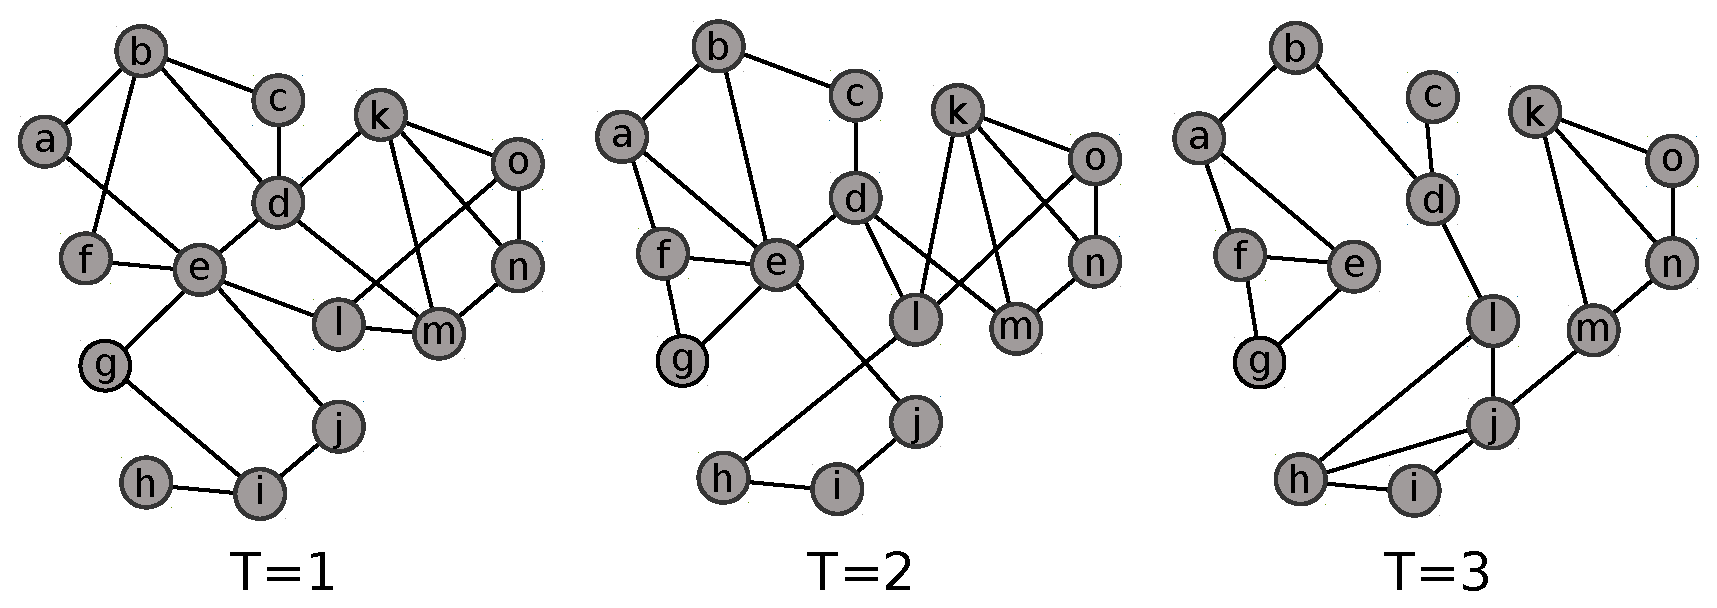
\includegraphics[width=0.8\linewidth]{img/Intro/TVG.eps}
\caption{Exemple de série de graphes sur trois intervalles de temps.}
\label{fig:exemple_TVG}
\end{figure}
La première solution qui a été apportée ne prend le temps en compte que partiellement.
Il s'agit de manipuler une série de graphes où chaque graphe représente le réseau durant un intervalle de temps donné.
Ainsi, il est possible d'appliquer les outils de la théorie des graphes sur chaque intervalle.
Cependant chaque intervalle de temps est représenté par un graphe agrégé.
Il y a donc toujours une perte d'information.
Plus formellement, une série de graphe est définie par $\mathcal{G}=\{G_i\}_{i < T}$ où $T$ est un entier, voir l'illustration~\ref{fig:exemple_TVG}.

Cette définition initiale laisse le choix sur la découpe du temps en intervalle.
Il est possible de choisir des intervalles de tailles égales ou non et disjoints ou chevauchants~\cite{Wang2012}.
Utiliser des intervalles à durée variable permet de mieux tenir compte de la dynamique.
Par exemple lors de l'étude d'interactions de personnes, il est très courant d'observer une très faible activité la nuit et une plus forte la journée.
Un graphe agrégeant ce qui se passe sur un intervalle de 5h sera vide dans le premier cas et peut être trop dense dans le second.
La détection d'intervalle pertinent est donc un vaste sujet de recherche~\cite{Rosvall2010,Krings2012,Ribeiro2013,Caceres2013,Peel2015,de2016detection}.

La notion même de temps est importante.
Albano~\emph{et al.}~\cite{Albano2014} propose d'utiliser une autre mesure que la seconde mais plutôt le nombre de changements comme mesure du temps.
Ainsi, le temps n'avance pas si aucun changement n'a lieu et au contraire il avance beaucoup si énormément de changements apparaissent.
Cette manière de procéder se rapproche des travaux de Lamport~\cite{Lamport1978} dans les systèmes distribués.

\paragraph{Détection de communautés}
Dans ce contexte de série de graphes, il y a eu assez tôt des méthodes de détection de communautés~\cite{Hopcroft2004,Sun2007,Lin2008,Asur2009}.
Il est, en effet, assez naturel d'appliquer une méthode de détection statique sur chaque graphe puis d'essayer de faire du suivi de communautés.
Le suivi de communautés consiste à comprendre comme une communauté donnée évolue, étant donné une série de graphes et une série de partitions.
Palla~\emph{et al.}~\cite{Palla2007} ont été parmi les premiers à décrire les évolutions possibles d'une communauté.
Muni d'indicateurs de similarité tels que l'indice de Jaccard, voir~\ref{def:graphe_comparaison}, il est possible de trouver les communautés les plus proches aux instants précédent et suivant.
\`A partir de ces informations, 5 type d'évolutions d'une communauté sont définis:
\begin{description}
\item[Naissance] Une nouvelle communauté apparait.
\item[Agrandissement] La communauté continue d'exister et s'agrandit.
\item[Fusion] Deux communautés fusionnent pour donner lieu à une nouvelle communauté.
\item[Division] Une communauté se sépare en deux nouvelles communautés à l'étape suivante.
\item[Mort] Une communauté cesse d'exister dans les graphes suivants.
\end{description}

Ce type de méthodes souffre souvent de l'instabilité des méthodes de détection~\cite{Aynaud2010,Harenberg2014a}.
Si les partitions changent complètement entre deux graphes consécutif, alors il est difficile de faire un réel suivi de communautés.
C'est pourquoi des méthodes essayent de forcer une certaine stabilité de la partition en ajoutant un coût de transition~\cite{Chakrabarti2006,Chen2013,Kalavathi2015}.
Une approche détournée pour garder une certaine stabilité est d'utiliser la partition trouvée précédemment comme base de recherche pour l'intervalle suivant~\cite{Lancichinetti2011a}.

Des extensions des Stochastic Block Models ont également été proposées par différents auteurs dans le cadre des séries de graphes.
Yang~\emph{et al.}~\cite{Yang2011} sont parmi les premiers à considérer ce cas de figure.
Ils considèrent que la probabilité d'un lien entre deux communautés est fixe et que ce qui change est l'affiliation des n\oe uds au cours du temps.
Ce processus de changement de communauté suit alors une chaine de markov cachée.
\`A l'inverse, Corneli~\emph{et al.}~\cite{Corneli2016} considèrent une partition de n\oe uds fixe tout au long du temps et c'est l'activité entre deux communautés qui change selon l'intervalle de temps.
Xu~\emph{et al.}~\cite{Xu2014} permettent à l'affiliation et à l'activité entre deux communautés de changer selon l'intervalle de temps.
Cependant, il semblerait que cette relaxation se fasse au dépens de l'identifiabilité des paramètres d'après Matias~\emph{et al.}~\cite{Matias2015}.
Ils ont donc proposé une nouvelle méthode afin de résoudre ce problème.
De plus, leur méthode permet de traiter des séries de graphes pondérés.

\subsubsection{Tenseur 3D}
Les tenseurs 3D ne sont pas en soi différents des séries de graphes.
Il est possible de voir un graphe comme une matrice carrée d'adjacence.
Il est donc normal de concevoir une série de graphes comme un tenseur appartenant à $\mathcal{R}_{nnT}$.
Ce changement de point de vue permet ainsi d'appliquer les méthodes d'algèbre linéaire, notamment la décomposition de tenseur.
C'est la méthode proposée par Gauvin~\emph{et al.}~\cite{Gauvin2014} pour étudier la structure communautaire des interactions d'élèves.
Cependant ce genre de décomposition semble moins expressive que les SBM.


\subsubsection{Graphes multicouches}
\begin{figure}[h]
\centering
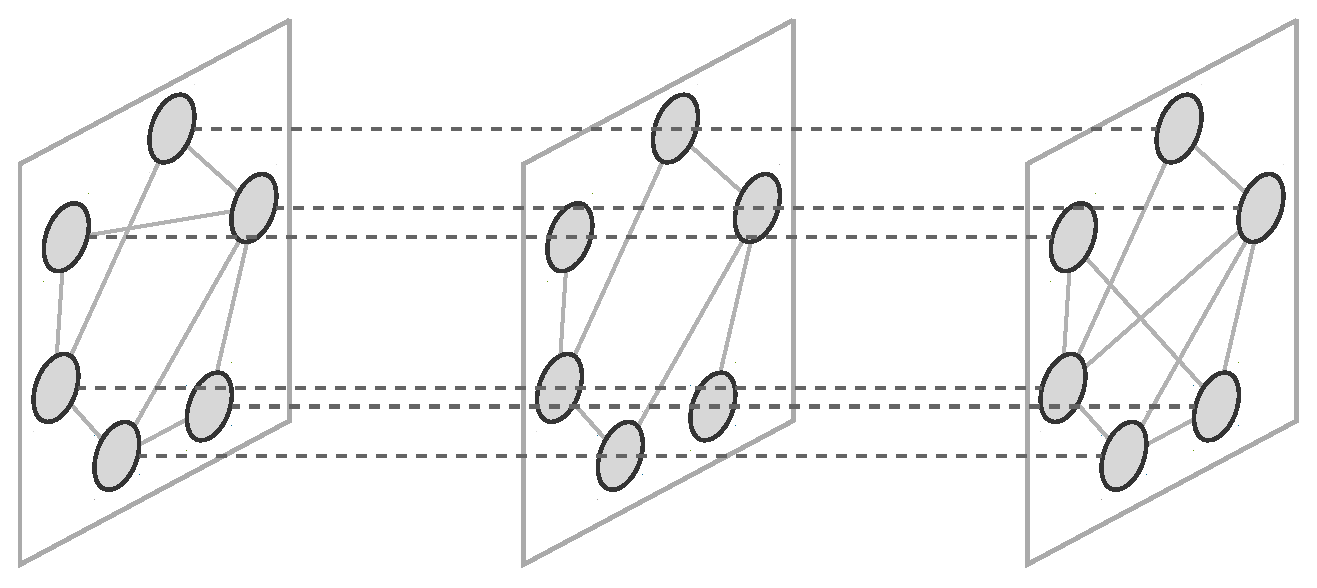
\includegraphics[width=0.7\linewidth]{img/Intro/multiplex.eps}
\caption{Graphe multicouche avec trois couches représentant le temps.
Les liens pleins (resp. pointillés) sont les liens intra-couches (resp. inter-couches).}
\label{fig:exemple_multiplex}
\end{figure}
La construction de graphes multicouches (\emph{multilayer} ou \emph{multiplex}) est proche de l'idée des séries de graphes.
Tout comme les séries de graphes, des n\oe uds et des liens sont créés à chaque intervalle pour représenter ce qui s'est déroulé durant l'intervalle de temps.
Cependant, le graphe multicouches ajoute des liens entre les n\oe uds de deux intervalles, voir l'illustration~\ref{fig:exemple_multiplex}.
Par conséquent, un graphe multicouches est un graphe où il existe deux types de liens, les liens intra-couches et les inter-couches et il existe $T$ répliques d'un même n\oe ud, une par intervalle de temsp.
Les liens intra-couches représentent un connexion entre deux n\oe uds durant un intervalle de temps.
Les liens inter-couches représentent un lien entre deux n\oe uds sur deux intervalles différents.
Ces derniers sont utilisés pour identifier un même n\oe ud sur plusieurs intervalles et sont en général limités à relier deux couches consécutives.

Les graphes multicouches représentent les données évoluant dans le temps mais ils modélisent aussi très bien d'autres situations.
Par exemple, ils permettent de représenter facilement les différents moyens de transport dans une ville où chaque moyen de transport (bus, voiture, métro ...) est représenté par une couche.
Plusieurs travaux~\cite{DeDomenico2013,Kivela2014,Boccaletti2014} décrivent les graphes multicouches et leurs applications.



\paragraph{Détection de communautés}
Grâce au formalisme de graphe multicouches, il est possible de traiter le temps de manière un peu plus fine que dans les séries de graphes car il permet de mieux suivre l'évolution des n\oe uds.
Comme un graphe multicouches est un graphe, il est possible d'adapter les méthodes existantes pour tenir compte des différents types de liens.
C'est le cas d'infomap~\cite{DeDomenico2014}, de la modularité~\cite{Mucha2010,Bassett2013,Bazzi2016} et du SBM~\cite{Stanley,Peixoto2015c}.


\resume{
Les séries de graphes, les tenseurs et les graphes multicouches permettent de prendre en compte le temps tout en autorisant l'utilisation de méthodes conçues sur un graphe statique.
Cette liberté d'utilisation a un coût.
Ces approches reposent sur une découpe du temps en sous-intervalles durant lesquelles le temps n'est plus pris en compte afin d'obtenir un graphe statique.
Or, il peut être délicat de définir ces intervalles de temps.
De plus, la construction des graphes agrégés entraine une perte d'information temporelle et cela impacte la précision temporelle des structures communautaires qui sont manipulables.
Il n'est pas envisageable d'augmenter le nombre d'intervalles de temps car cela induirait d'une part des graphes agrégés avec très peu de liens et d'autre part le temps de calcul serait très fortement impacté.
}

\subsection{Extension sans perte d'information temporelle}
\label{subsec:pasperte_info}
\subsubsection{Graphe temporel}
\begin{figure}[h]
\centering
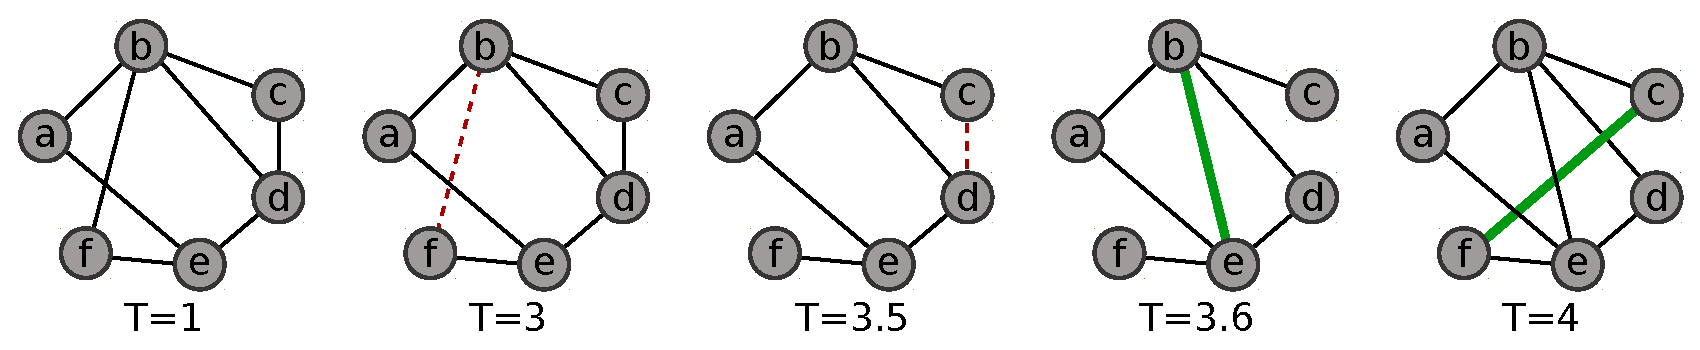
\includegraphics[width=0.9\linewidth]{img/Intro/evolvingGraph.eps}
\caption{Graphe temporel avec des ajouts de lien représentés en trait épais vert et des retraits de lien représentés par des liens pointillés rouge.
}
\label{fig:exemple_evolving}
\end{figure}
Les graphes temporels (\emph{Time Varying Graph} ou \emph{Evolving Graph})
permettent de tenir compte de l'ensemble de l'information temporelle.
Pour cela au lieu de considérer des intervalles de temps, ils considèrent l'ensemble des modifications qui affectent le graphe: les ajouts et retraits de liens.
En pratique, cela revient à considérer sur chaque lien une fonction de présence en fonction de temps qui vaut $1$ à un instant $t$ si le lien existe à cet instant et $0$ sinon.
Ainsi, il est possible de connaitre la structure de graphe à chaque instant.
Ce formalisme est présenté dans différents travaux~\cite{Casteigts2011,Wehmuth2015} et illustré dans la figure~\ref{fig:exemple_evolving}.
Dans cette figure, on voit apparaitre l'ordre de modification du graphe.
Tout d'abord, les lien $(b,f)$ et $(c,d)$ disparaissent puis les liens $(b,e)$ et $(f,c)$ apparaissent chacun leur tour. 

\paragraph{Détection de communautés}
Dans un graphe temporel, une structure de graphe existe à chaque instant.
Il est donc possible de calculer après chaque modification l'évolution d'une métrique.
Par exemple, il est possible de calculer après l'ajout d'un lien le nouveau degré interne des n\oe uds impactés par ce changement.
En fonction de l'évolution de cette métrique, il est alors décidé d'ajouter ou retirer un n\oe ud voire de fusionner deux communautés.
Li \emph{et al.}~\cite{Li2012a} se base sur le nombre de liens que partage un n\oe ud avec les communautés environnantes.
Ainsi, un n\oe ud est toujours dans la communauté avec laquelle il partage le plus de liens.
Shang\emph{et al.}~\cite{Shang2014a}, Cordeiro~\emph{et al.}~\cite{Cordeiro2016} et Sun\emph{et al.}~\cite{Sun2014} se basent sur l'évolution de la modularité.
Cependant, ces approches ne permettent pas l'ensemble des évolutions de communauté possibles, en particulier l'apparition d'une nouvelle communauté.
C'est pourquoi l'évolution de la structure courante peut mener à une structure ayant une faible qualité.
Une autre approche a été proposée par Cazabet~\emph{et al.}~\cite{Cazabet2010} afin d'améliorer l'évolution de la partition.
Ils utilisent une métrique locale basée sur le nombre de chemins de longueur $2$ existant entre un n\oe ud et une communauté.
Après chaque modification, ils considèrent également la possibilité de créer une nouvelle communauté sous la forme d'une petite clique.
Ainsi, ils assurent une meilleure qualité de la partition au cours de l'évolution.


\subsubsection{Flot de liens}
\begin{figure}[h]
\centering
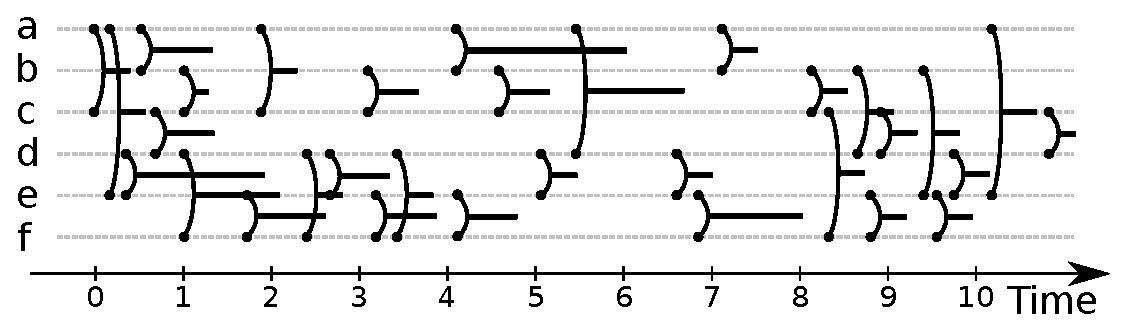
\includegraphics[width=0.9\linewidth]{img/Intro/Flot_de_liens.eps}
\caption{Flot de liens entre $6$ n\oe uds, représentés sur l'axe des ordonnées, au cours du temps représenté sur l'axe des abscisses.
Dans l'exemple, il existe un lien entre $a$ et $b$ durant l'intervalle $[4,6]$.
}
\label{fig:exemple_Flot_de_liens}
\end{figure}
Dans les graphes temporels, toute l'information temporelle est gardée.
Cependant, l'intuition derrière cette méthode est qu'il existe une structure de graphe à chaque instant.
Cette hypothèse n'est pas toujours vérifiée, en particulier lorsque les liens apparaissent et disparaissent très rapidement.
C'est le cas des appels téléphoniques qui durent rarement plus d'une heure ou bien de manière plus frappante avec les SMS et les courriels qui n'ont même pas de durée.
Dans ces contextes, il n'est pas possible de supposer qu'à chaque instant une structure de graphe existe.
Il faut donc un formalisme et des mesures qui s'adaptent à ce contexte.
C'est pour répondre à ce besoin que le formalisme de flot de liens a été pensé.
Le but est de construire un objet ne présupposant aucune structure et qui stocke toute l'information disponible.
Même si le formalisme ne présuppose aucune contrainte structurel, il se peut en revanche que le reseau représenté en ait.
Par exemple dans les télécommunications, une personne ne peut appeler qu'une ou deux personnes en même temps.
Plusieurs travaux~\cite{Holme2013a,Holme2015b,Holme2015e} font un tour d'horizon des méthodes existantes pour étudier les flots de liens qui sont souvent appelés \emph{temporal networks} mais il n'existe, à notre connaissance, qu'un seul travail donnant un fondement théorique solide au flot de liens.
Il s'agit de Batagel~\emph{et al.}~\cite{Batagelj2016} qui se basent sur l'algèbre.
Malheureusement avec une formulation purement algébrique, il semble difficile de transcrire l'ensemble des notions de graphes pour l'instant.
\bigskip

Prenons l'exemple des appels téléphoniques, c'est-à-dire qui parle avec qui à quelle heure et pendant combien de temps.
Un appel peut donc être représenté par un quadruplet $(b,e,u,v)$ où $b$ (res. $e$) est le début (resp. la fin) de l'appel et $u$ et $v$ représentent des personnes.
Il est donc possible de modéliser des appels téléphoniques par un ensemble de quadruplet.
En faisant cela, aucune information n'est perdue et, en ce sens, flots de liens et graphes temporels sont équivalents. 
Cependant, ce changement de perspective induit une réflexion différente selon le formalisme considéré.

Les différences dans les méthodes de représentation des graphes temporels de la figure~\ref{fig:exemple_evolving} et celle des flots de liens de la figure~\ref{fig:exemple_Flot_de_liens} illustrent bien ce changement de perspective, bien que les deux figures ne représentent pas le même réseau.
Dans l'exemple de la figure~\ref{fig:exemple_Flot_de_liens}, les n\oe uds sont représentés sur l'axe des ordonnées et le temps sur l'axe des abscisses.
Un lien dans cette visualisation est représenté par: un arc vertical reliant deux axes de n\oe uds et un trait horizontal représentant la durée du lien.
Ainsi dans l'exemple, il existe un lien entre les n\oe uds $a$ et $b$ dans l'intervalle $[4,6]$.

Dans un graphe temporel, on abordera plus souvent les questions d'évolution de communautés de n\oe uds ou de l'importance d'un n\oe ud.
Dans un flot de liens, on s'intéressera plus souvent au temps nécessaire pour que deux n\oe uds soient de nouveau en contact ou à l'importance d'un lien.
De manière très manichéenne et inexacte, le formalisme de graphe temporel pousse à étudier les relations et leur évolution alors que celui de flot de liens mets plus l'accent sur les interactions et leur dynamique.

\bigskip



Avec ce formalisme, la majorité des travaux sont encore descriptifs car ce type d'objet n'a jamais été étudié sous cet angle.
Il existe de nombreux travaux étudiant le temps séparant l'apparition de deux liens pour un n\oe ud~\cite{Malmgren2008,Malmgren2009}.
Il semblerait que ces temps inter-contacts soient très hétérogènes et que de nombreuses connexions apparaissent dans un faible intervalle de temps suivie de longues durées sans activité.
On parle alors de temps inter-contact \emph{bursty}.
Les effets des temps inter-contacts sur les phénomènes de diffusions et de marches aléatoires sont très étudiés~\cite{Karsai2011,Karsai2012a,Starnini2012b,Rocha2013}.
Il semble cependant ne pas y avoir de conclusion définitive sur le sujet car la diffusion peut être accélérée ou ralentie par les temps inter-contacts selon la structure sous-jacente.

Il existe également quelques méthodes qui s'intéressent plus à la structure des flots de liens.
Des études~\cite{Kovanen2011a,Kovanen2013a} s'intéressent à la présence de motifs.
Un motif dans un graphe est un petit sous-graphe comme le triangle qui est l'un des motifs les plus étudiés.
Dans les flots de liens, le temps est également pris en compte dans les motifs.
Il y a donc plusieurs variantes temporelles d'un même motif dans un graphe.
Prenons l'exemple d'un chemin entre quatre n\oe uds $A$, $B$, $C$ et $D$ qui est représenté dans le graphe par  $\{(A,B), (B,C), (C,D)\}$.
Dans un flot de liens, il existe deux variantes à ce motif soit
$\{(t_1,A,B), (t_2,B,C), (t_3,C,D)\}$ soit $\{(t_1,A,B), (t_2,C,D), (t_3,B,C)\}$ avec $t_1<t_2<t_3$.
Dans un cas,  une information peut être propagée au fur et à mesure de $A$ vers $D$ tant dis que dans l'autre ce n'est pas possible.
L'étude de la fréquence d'apparition de ces motifs dans le cas temporel permet d'observer si le flot de liens à une structure particulière. 



\paragraph{Détection de structures}
Il existe peu de méthodes détectant des structures décrivant l'ensemble d'un flot de liens.
Rozenshtein~\emph{et al.}~\cite{rozenshtein2014} se penchent sur la détection de la zone la plus dense dans les flots de liens.
Ils permettent de capturer un ensemble de n\oe uds et plusieurs intervalles de temps disjoints tel que ces n\oe uds sur ces intervalles aient le degré moyen le plus élevé dans le graphe agrégé sur ces intervalles.
Bien que la mesure utilisée ne tienne pas directement compte du temps, leur méthode permet ainsi de mettre en évidence une partie du flot de liens.

\cite{Viard2016,viard:hal-01208330}

Une méthode de type Stochastic Block Model a été proposée par Matias~\emph{et al.}~\cite{Matias2015a}.
Elle est très proche de celle proposé par Corneli~\emph{et al.}~\cite{Corneli2016}.
En effet, l'affiliation des n\oe uds est fixe et c'est l'activité d'une communauté qui change au cours du temps.
La grosse différence ici est que l'activité varie de manière continue dans le temps.
Ainsi l'apparition d'un lien dépend de la réalisation d'un processus de Poisson non homogène qui change selon les communautés.
Cependant, leur méthode ne permet pas de considérer les changements de communauté.

% centralité \cite{,Kim2012, Pfitzner2013a,Praprotnik2015,Scholtes2015,Costa2015,Takaguchi2016}

\resume{
Les graphes temporels et les flots de liens ne souffrent pas d'agrégation temporelle.
Ils ont donc un pouvoir expressif plus important que les formalismes présentés précédemment.
Formellement, flots de liens et graphes temporels sont équivalent dans le sens où un graphe temporel peut être représenté en un flot de liens et \emph{vice versa}.
En revanche, ils diffèrent dans le point de vue considéré.
Dans un graphe temporel, il existe une structure de graphe représentant le réseau à chaque instant et les métriques de graphes sont pertinentes.
Dans un flot de liens, il n'existe pas de structure pertinente à un instant donné et par conséquent les métriques de graphes ne sont pas pertinentes dans ce contexte.
Cette différence implique d'utiliser des mesures différentes et, en particulier, de créer de nouvelles métriques pour les flots de liens.
Cela explique notamment pourquoi il n'existe pour l'instant qu'assez peu de travaux traitant de la structure des flots de liens.
Cette différence de perspective entraine également un déplacement du centre d'intérêt.
Dans les graphes temporels, on aura plutôt tendance à étudier les relations et leur évolution.
\`A l'inverse, on s'intéresse plutôt aux interactions et leur répartition dans les flots de liens.
Ainsi, les deux formalismes coexistent et répondent à des besoins différents.}

\section{Bilan}

Dans un graphe statique, il existe de très nombreuses méthodes capturant une structure des n\oe uds soit via une partition soit via une couverture.
L'abondance de méthodes existantes s'explique par la diversité des définitions de communautés existantes.
Les structures capturées permettent de mieux comprendre l'organisation générale du graphe mais aussi de mieux comprendre le type d'un n\oe ud.


Avec l'émergence de nouvelles données incorporant l'information temporelle, il est pertinent d'adapter la théorie des graphes pour prendre en compte le temps.
L'extension temporelle des graphes est un champ de recherche très récent et il n'y a pas à douter que de nombreuses méthodes de détection de communautés dans ce contexte vont voir le jour.
Cependant, tout les formalismes existants ne sont pas équivalents et ils limitent parfois les solutions possibles.


Il y a d'une part les formalismes se rapprochant de la théorie des graphes: séries de graphes, tenseurs 3d et graphes multicouches.
Ces formalismes sont proches des graphes statiques et il est même possible d'y appliquer des méthodes statiques.
En revanche, la prise en compte du temps n'est que partielle.
Il y a toujours une forme agrégation temporelle et il n'est pas possible d'avoir une vision très fine de l'objet d'étude.
De plus, les solutions existantes reposent sur le suivi de communautés qui ne semble pas être un problème résolu.


D'autre part, les formalismes de graphes temporels et de flots de liens capturent toute l'information temporelle.
Ils ne souffrent donc pas de perte d'information.
Ces deux formalismes, bien qu'équivalent, ne présupposent pas la même structure sur les données sous-jacentes.
Dans un graphe temporel, les liens durent assez longtemps et par conséquent il existe une structure de graphe pertinente à chaque instant.
Dans les flots de liens, les liens sont plus courts et il n'existe aucune structure de graphe à un instant donné.
Par conséquent, ces deux formalismes répondent à des situations différentes.
Par exemple, les études des temps inter-contacts sont très majoritairement conduites en utilisant le formalisme de flot de liens.
Il semble donc plus aisé d'utiliser un flot de liens qu'un graphe temporel lorsque l'on souhaite étudier la structure des interactions.



Au cours de cette thèse, nous nous intéressons à la structure communautaire que peuvent former les liens dans le temps.
Nous ne pouvons pas utiliser les formalismes utilisant une agrégation temporelle car l'identité du lien est perdue et le formalisme de graphe temporel considère des situations assez différentes de celles que nous étudions.
C'est pourquoi le formalisme de flot de liens semble être le plus adapté pour étudier la structure des liens.
Il n'existe que peu de travaux définissant formellement les flots de liens et traitant de leur structure.
C'est pourquoir dans le chapitre~\ref{chap:def_flot}, nous définissons plus formellement ce qu'est un flot de liens ainsi que les métriques utilisées tout au long de cette thèse avant de présenter nos travaux sur la structure des liens dans les chapitres suivants.




\chapter{Flots de liens: extension temporelle des graphes}
\minitoc
\label{chap:def_flot}

\section{Définition}
\label{sec:definition}

Nous avons décrit rapidement le formalisme de flot de liens dans le chapitre précédent.
Nous nous attachons maintenant à définir plus formellement les flots de liens et quelques notions qui s'y appliquent.
Un flot de liens est défini comme un triplet: $\mathcal{L}=(T,V,E)$, où $T=[\alpha, \omega]$ est un intervalle de temps, $V$ un ensemble de $n$ n\oe uds et $E\subseteq T\times T \times V \times V$ un ensemble de $m$ liens.
Les liens de $E$ sont des quadruplets $(b,e,u,v)$, signifiant que la paire de n\oe uds $(u, v)$ est connectée sur l'intervalle $[b,e] \subseteq [\alpha,\omega]$.
Nous dénotons la durée du flot par $\bar{L}=\omega-\alpha$.
De manière analogue, la durée d'un lien $l=(b,e,u,v) \in E$ est notée   $\bar{l}=e-b$.
$\beta(E)= min_{(b,e,u,v) \in E} (b)$ et $\psi(E)= max_{(b,e,u,v) \in E} (e)$ sont respectivement l'apparition du premier lien et la disparition du dernier lien.

Nous considérons les flots de liens non orientés, \emph{i.e.} $(b,e,u,v)=(b,e,v,u)$, et sans boucle, \emph{i.e.} $u \neq v$.
Enfin de manière analogue aux graphes et multigraphes, nous définissons les flots de liens simples.
Un flot de liens est simple si pour tout $l_1=(b,e,u,v) \in E$ et $l_2=(b',e',u, v) \in E$, $[b,e]\cap [b', e'] = \emptyset$ si $l_1 \neq l_2$.
Dans les graphes, il est possible de transformer un multigraphe en graphe simple.
Nous définissons également cette opération que nous nommons simplification: $\sigma(L)$.
Afin de définir la simplification, nous nous aidons de la fonction de présence $\zeta_{L}(u,v,t)$ d'un flot de liens qui est égale à $1$ si au moins un lien existe dans le flot $L$ entre $u$ et $v$ à l'instant $t$ et $0$ sinon
$L'=(T',V',E')$ est la simplification de $L=(T,V,E)$ si et seulement si $L'$ est simple, $T'=T$, $V'=V$ et $\forall u,v \in V,\ \forall t\in T, \zeta_{L}(u,v,t)= \zeta_{L'}(u,v,t)$.

Enfin, il est parfois d'allonger la durée des liens.
C'est notamment utile lorsque les liens sont de la forme $(t,t,u,v)$, ce qui est le cas lorsqu'on étudie des envoies de courriels par exemple.
Nous notons $\xi(L,\Delta)=L'$ le fait d'allongé de $\Delta$ chaque lien.
Il y a plusieurs moyen d'agrandir de $\Delta$ un intervalle $[b,e]$.
Nous considérons l'ajout symétrique c'est à dire qu'un intervalle $[b,e]$ est transformé en l'intervalle $[b-\Delta/2,e+\Delta/2]$.

Une fois défini les flots de liens, nous pouvons commencer à définir différentes opérations pour les analyser.


\section{Sous-flots}
Dans les graphes, il existe la notion de sous graphes que nous étendons également aux flots de liens.
Un flot de liens $L'$ est un sous-flot de $L$, $L' \subset L$, si  $\forall u,v \in V,\ \forall t\in T, \zeta_{L'}(u,v,t) < \zeta_{L}(u,v,t)$.
Cette notion est en particulier utile pour définir des sous-flots induits par différent éléments.
Nous illustrons ces notions dans la figure~\ref{fig:exemple_sous_flot} avec le flot initial dans la figure~\ref{fig:exemple_sous_flot_init}.
 
Nous définissons $L(E')$ , le sou-flot de $L$ inuit par un ensemble de liens $E' \subset E$: $L(E')=([\beta(E'),\psi(E'),V(E'),E'])$.

 
Nous définissons $L(S)$ , le sou-flot de $L$ induit par un ensemble de paire n\oe uds $S \in V^ 2$: $L(S)$: $L(S)=([\beta(E'),\psi(E')],V',E')$ avec $E'= \{(b,e,u,v) \in E, (u,v) \in S\}$.
Un exemple de sous-flot induit par un ensemble de n\oe uds est dans la figure~\ref{fig:exemple_sous_flot1}.
Par abus de notation, on note $L(v)= L(\{v\}\times V)$, le sous-flot induit par un n\oe uds.


Enfin, nous définissons $L_{t..t'}$, le sous-flot de $L$ induit par l'intervalle de temps $[t,t'] \subset [\alpha, \omega]$: $L_{t..t'}=([t, t'], V,E')$ avec $E'= \{(b',e',u,v),\ \exists (b,e,u,v) \in E,\ b'= max(b,t),\ e'=min(e,t')\}$.
Il est également possible de définir $L_{t..t'}$ via la fonction de présence: $\forall u,v \in V,\ \forall x \in [t,t']\  \zeta_{L_{t..t'}}(u,v,x) = \zeta_{L}(u,v,x)$.
Un exemple de sous-flot induit par un intervalle de temps est dans la figure~\ref{fig:exemple_sous_flot2}.
Il est intéressant de noter que le sous flot $L_t..t$ est équivalent au graphe statique à l'instant $t$,  que nous notons $G(L_t)$.


\begin{figure}[]
\centering
	\begin{subfigure}{0.2\linewidth}
		
\includegraphics[width=\linewidth]{img/Intro/sous_flots.eps}\hfill
		\caption{Flot de liens initial $L$}
		\label{fig:exemple_sous_flot_init}	
	\end{subfigure}\hspace{0.1\linewidth}
	\begin{subfigure}{0.2\linewidth}
		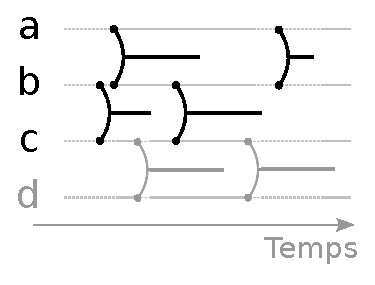
\includegraphics[width=\linewidth]{img/Intro/sous_flots1.eps}\hfill
		\caption{Sous-flot induits par des n\oe uds: $L({a,b,c}^2)$}	
		\label{fig:exemple_sous_flot1}	
	\end{subfigure}\hspace{0.1\linewidth}
	\begin{subfigure}{0.2\linewidth}
		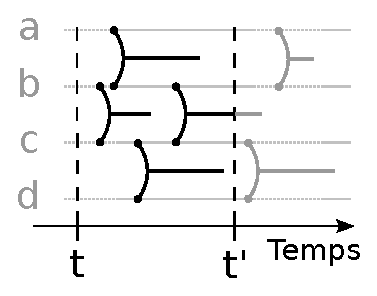
\includegraphics[width=\linewidth]{img/Intro/sous_flots2.eps}\hfill
		\caption{Sous-flot induits par le temps:  $L_{t..t}$}
		\label{fig:exemple_sous_flot2}	
	\end{subfigure}
	\caption{Exemple de différents sous-flots, (B) et (C), du flot initial en (A). Les liens en noirs sont les liens sélectionnés dans le sous-flot. }
\label{fig:exemple_sous_flot}
\end{figure}
Il est aussi possible de combiner ces notions.
Par exemple avec $V' \subset V$, $L_{\alpha'..\omega'}(V'^2)$ est le sous flot correspondant au lien entre les n\oe uds de $V'$ sur l'intervalle $[\alpha', \omega']$.
\bigskip
Enfin de il est intéressant de noter que la construction de ces sous flots peut être fait de manière sous linéaire au nombre de liens total pour les sous flots induits par un ensemble de n\oe uds, un ensemble de liens mais pas pour un intervalle de temps.
Pour l'ensemble de n\oe uds, il suffit d'itérer sur l'ensemble des liens qui sont reliés à un des n\oe uds de l'ensemble.
Cela peut être fait rapidement si chaque n\oe uds a la connaissance des ces liens.

Pour l'intervalle de temps, la situation est plus compliquée car il n'existe d'ordre total des liens que sur leur apparition ou sur leur disparition.
Il n'y a pas d'ordre total sur la présence qui permettrait de considérer uniquement les liens appartenant au sous flot.
Pour qu'un lien, $l= (b,e,u,v)$ appartienne au sous flot temporel sur $[t,t']$, il doit remplir une des ces conditions, qui ne sont pas exclusives:
\begin{description}
\item[$t \leq b \leq t'$] le lien commence dans l'intervalle $[t,t']$.
\item[$t \leq e \leq t'$] le lien fini dans l'intervalle $[t,t']$.
\item[$ b \leq t \, \wedge \, t' \leq e$] le lien couvre tout l'intervalle $[t,t']$.
\end{description}

Avec ces conditions, on peut tirer deux conclusions.
Pour qu'un lien $l=(b,e,u,v)$ puisse appartenir au sous flot, il est nécessaire que $e \geq t$.
Il n'est donc pas nécessaire de considérer les liens ayant un temps de fin inférieur à $t$.
De manière analogue, il n'est pas nécessaire de considérer les liens ayant un temps de début supérieur $t'$.
Cependant ces deux conditions ne peuvent pas être combinées pour restreindre l'espace de recherche.
Une manière de construire le sous flot temporel est d'itérer sur tous les liens dans l'ordre temporel d'apparition et d'arrêter le parcours dès qu'un lien a un temps de début supérieur à $t'$.
Il faut cependant tester l'appartenance de chaque lien parcouru.
De manière analogue, il set possible d'itérer sur les liens dans l'ordre inverse de disparition des liens et de s'arrêter dès qu'un lien a une temps de fin inférieur à $t$.


Dans le pire des cas, ces méthodes sont donc linéaire sur le nombre total de liens dans le flot et non dans le sous flot comme précédemment.
La seul optimisation possible est le choix du sens du parcours si les deux ordres sont disponibles.



\section{Degré et densité}
\label{sec:def_densite}
Nous avons défini des outils pour manipuler et extraire un flot de liens.
Nous nous intéressons maintenant à étendre quelques notions de connexité qui existe dans le graphe, en particulier le degré et la densité.

Il est assez trivial de définir le degré temporel d'un n\oe ud $u$ de la manière suivante:
\begin{equation}
d(t,u)=d_t(u)= |L_t(u)|= \sum_{v \in V} \zeta_{L}(u,v,t).
\end{equation}
Le degré temporel n'est pas une simple valeur mais une fonction qui dépend du temps.
Comme les liens apparaissent et disparaissent de manière instantanée, la fonction de degré est une fonction constante par morceaux.
Un exemple de degré temporel est présenté dans la figure~\ref{fig:exemple_degre}.

\begin{figure}
\centering
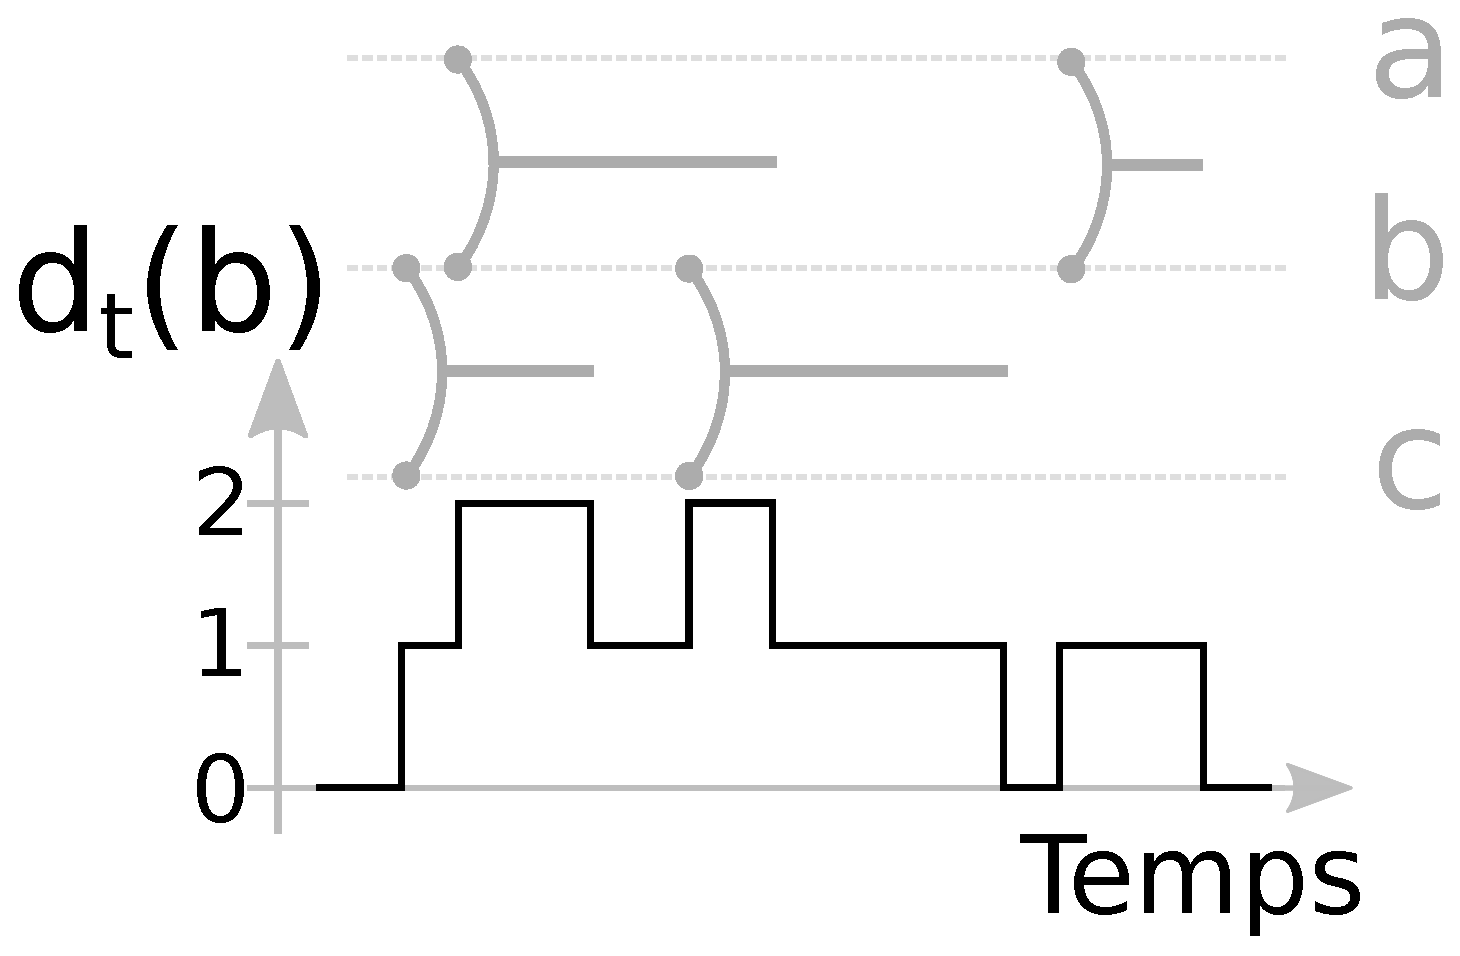
\includegraphics[width=0.5\linewidth]{img/Intro/degre2.eps}
\caption{Degré temporel du n\oe ud $b$ dans le flot de liens dans la figure~\ref{fig:exemple_sous_flot_init} qui est également rappelé en grisé dans cette figure.
}
\label{fig:exemple_degre}
\end{figure}

De manière analogue aux graphes, il est également possible de définir le degré temporel d'un ensemble de n\oe uds ou d'un ensemble de liens:

\begin{equation}
d_t(V')= \sum_{v \in V'} d_t(v) = 2 |L_{t}(V'^2)| = 2|\{(b,e,u,v) \in E,\ u,v \in V',\ b \leq t \leq e\}|\,,
\end{equation}

\begin{equation}
d_t(E')=2|L_{t}(E')|= 2|\{(b,e,u,v) \in E',\ b \leq t \leq e\}|\,.
\end{equation}

Avec ces définitions, il est aussi possible définir les notions de degré temporel interne, $d_t^{in}$, et externe $d_t^{out}$.
Les degrés temporels d'un n\oe uds, d'un ensemble de n\oe uds ou de liens peuvent se calculer rapidement.
Pour ce faire, il faut d'abord transformer les liens $(b,e,u,v)$ en une suite de modifications de la forme $(b,u,v,+1)$ et $(e,u,v,-1)$ ce qui coûte $O(m)$.
Une fois cette liste créée, il suffit d'ordonner ces modifications dans l'ordre temporelle, $O(2mlog(2m))$, puis d'itérer sur l'ensemble des modification en sommant au fur et à mesure les apparitions et disparition de lien, $O(2m)$.
\bigskip

Les degrés sont des fonctions du temps mais il est souvent intéressant de regarder la valeur moyenne du degré:
\begin{equation}
d_{t..t'}(u)=\dfrac{1}{t'-t}  \int_{t}^{t'}d(u,t) dt = \sum_{l \in L_{t..t'}(u)} \dfrac{\bar{l}}{t'-t} \, .
\label{eq:deg_moyen}
\end{equation}

Lorsque cela n'est pas ambigu, nous notons $d_{\alpha..\omega}(u) = d(u)$.
Il est intéressant de noter dans cette formulation que si tout les liens durent tout au long du flot de liens alors le degré dans le graphe agrégé et le degré moyen dans le flot de liens sont égaux, c'est-à-dire  $d_{\alpha..\omega}(u) = d_G(u), \forall u \in V$.

\'A partir du degré, il est possible de définir beaucoup de notions différentes et notamment la densité.
Pour rappel, la densité dans un graphe est définie par $\delta(G)=2m/(n(n-1))=d(V)/(n-1)$ et est égale à la probabilité qu'il existe un lien entre 2 n\oe uds.
Si l'on transpose l'idée au formalisme de flot de liens, la densité dans un flot de liens est la probabilité qu'il existe un lien entre 2 n\oe uds à un instant donné aléatoire.
Cela se traduit par la formule suivante:
\begin{equation}
\delta(L)= \dfrac{2 \sum_{l \in E}\bar{l}}{n(n-1) (\omega-\alpha)}.
\end{equation}

Il se trouve que cette formulation est complètement équivalente à la densité moyenne des graphes $G(L_t)$:

\begin{equation*}
\dfrac{1}{\omega-\alpha} \int_{\alpha}^{\omega} \delta(G(L_t)) dt=
\dfrac{1}{\omega-\alpha} \int_{\alpha}^{\omega} \dfrac{d(t,V)}{(n-1)}dt=
 \dfrac{1}{\omega-\alpha} \int_{\alpha}^{\omega} \dfrac{\sum_{u \in V} d(t,u)}{n(n-1)}dt = 
 \dfrac{\int_{\alpha}^{\omega} \sum_{u \in V} d(t,u)dt}{n(n-1)(\omega-\alpha)} 
 \end{equation*}

 \begin{equation*}
 =
\dfrac{\sum_{u \in V} \int_{\alpha}^{\omega}d(t,u)dt}{n(n-1)(\omega-\alpha)} =
\dfrac{\sum_{u \in V} \sum_{l \in L_{t..t'}(u)} \bar{l}}{n(n-1)(\omega-\alpha)} =
\dfrac{\sum_{u \in V} \sum_{l \in L_(u)} \bar{l}}{n(n-1)(\omega-\alpha)}=
\dfrac{2\sum_{l \in E}\bar{l}}{n(n-1) (\omega-\alpha)} .
\end{equation*}

Pour arriver à ce résultat, nous utilisons la relation entre degré temporel moyen et somme des durées de l'équation~\ref{eq:deg_moyen} et le fait que la somme des degré soit égale à deux fois le nombre de liens.

La notion de densité que nous avons définie est donc cohérente avec notre notion de degré et traduit le même concept que dans les graphes.
De plus, la densité dans les flots de liens est aussi comprise entre à $0$ et $1$.
Enfin, cette formulation de densité est une généralisation de la densité proposée par Viard~\emph{et al.}~\cite{Viard2014a} qui ne considérait que les liens sans durée.

Le calcul de la densité d'un flot est linéaire en le nombre de liens car elle est dépendante du calcul de $d_{\alpha..\omega}(V)$  qui est fait de manière linéaire.
\clearpage
\section*{Liste des notations pour les flots de liens}
\begin{table}[h]
	\centering
	\begin{tabular}{|c|c|}
	\hline Symbole & description \\
	\hline $L$ & Flot de liens \\ 
	$T$ & intervalle de temps  \\
	$V$ & ensemble de n\oe uds\\
	$E$ & ensemble de liens: $(b,e,u,v)$ \\
	$n$ & nombre de n\oe uds  \\
	$|L|,|E|$ & nombre de liens dans le flot \\
	$\beta(E)$ & temps d'apparition du premier lien\\
	$\psi(E)$ & temps de disparition du dernier lien\\
	$\xi(L,\Delta)$ & Flot de liens où chaque lien dure $\Delta$\\
	$\sigma(L)$ & Simplification du flot de liens $L$\\
	$L(V'^2)$ & sous flot induits par les n\oe uds de $V'$ \\
	$L_{t..t'}$ & sous flot induits par l'intervalle $[t,t']$ \\
	$d_t(v)$ & degré de $v$ à l'instant $t$\\
	$d_t(C)$ & Somme des degrés des n\oe uds dans $V$ à l'instant $t$\\
	$d(v)$ & degré moyen $v$ sur $T$\\
	$\delta(L)$ & densité du flot\\
%	$\delta_{\Delta}(L)$ & densité du flot où chaque lien dure $\Delta$\\
	\hline
	\end{tabular} 
		\caption{Liste des notations pour les flots de liens}
\end{table}

\section{Manipulation concrète des flots de liens}

Nous avons défini formellement quelques notions pour les flots de liens.
Afin de manipuler ces notions simplement, nous avons mis en place une librairie capable de les calculer simplement.
Le but est de fournir une implémentation généraliste qui soit simple d'accès.
Ainsi, il sera possible à n'importe qui de calculer ces notions.
La démarche, bien que beaucoup plu modeste, est similaire à ce qui est fait avec les graphes et networkx\,\footnote{\url{https://networkx.github.io/}}.

L'implémentation est en \emph{C++} pour être rapide avec un export en \emph{python} pour faciliter l'utilisation.
Le code de cette implémentation est ligne\,\footnote{\url{XXX}} et la documentation également\,\footnote{\url{XXX}}.
Il est par exemple possible avec la librairie de lire un flot de liens et de calculer la densité moyenne d'un sous-ensemble de n\oe uds sur un intervalle arbitraire.
Comme le but de cette librairie est d'être généraliste, l'implémentation n'est pas optimisée en espace pour un calcul spécifique.
Ainsi il est aisé d'étendre la librairie en écrivant un nouveau calcul.
 

Un intérêt de cette implémentation est de permettre, en python, la génération de visualisation\,\footnote{Pour  l'instant, uniquement un export en svg est possible.}, voir le dessin dans la figure~\ref{fig:exemple_Flot_de_liens_lib}.
Parmi les possibilités offertes par la visualisation, il est possible de n'afficher qu'une partie des n\oe uds ou de ne garder qu'un sous intervalle de temps.
De plus, il est possible de choisir la couleur des liens de manière manuelle ou en fonction d'une partition de liens.

\begin{figure}
\centering
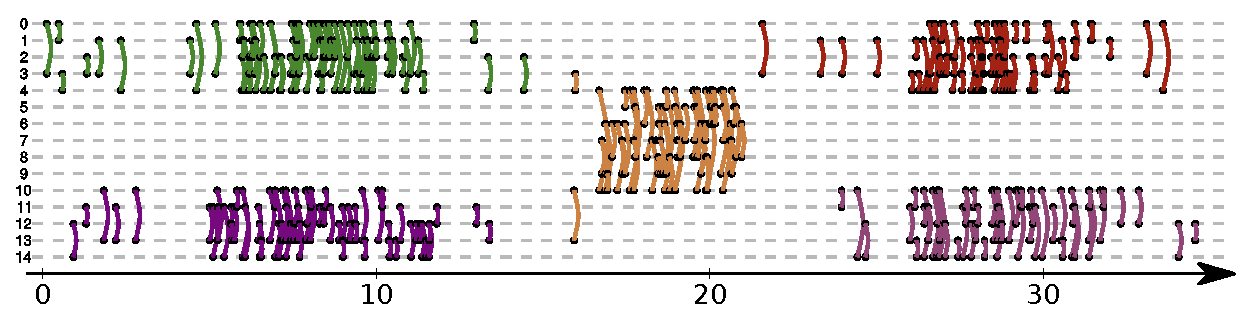
\includegraphics[width=\linewidth]{img/Intro/Dessin_Flot.eps}
\caption{Flot de lien entre $6$ n\oe ds, représenté sur l'axe des ordonées, au cours du temps représenté sur l'axe des abscisses.
Dans l'exemple, il existe un lien entre $a$ et $b$ durant l'intervalle $[4,6]$.
}
\label{fig:exemple_Flot_de_liens_lib}
\end{figure}

La lisibilité de ce genre de visualisation est très dépendant de l'ordre attribué aux n\oe uds sur l'axes des ordonnées.
C'est pourquoi avec notre outil, il est également possible de fixé un ordre arbitraire.
Comme il peut être fastidieux d'écrire un ordre, nous avons implémenté un algorithme rudimentaire pour améliorer l'ordonnancement des n\oe uds dans la visualisation.
Avant de pouvoir améliorer une visualisation, il est nécessaire de pouvoir quantifier la complexité de la visualisation actuel.
Empiriquement, on se rend vite compte que ce sont les long traits verticaux qui rende pénible la lecture et qu'il faut limiter.

C'est pourquoi nous décidons d'évaluer une ordonnancement en fonction de la somme des longueurs des traits représentant les liens.
Avec la fonction d'ordre $Ordre: V \longmapsto \mathbb{N}$, trouver le meilleur ordonnancement se résume à résoudre:

\begin{equation}
 Ordre* = \argmin_{Ordre}  \sum_{(b,e,u,v) \in E} |Ordre(u)- Ordre(v)|
\end{equation}

Malheureusement, trouver l'optimum ne semble pas trivial et il n'est pas envisageable de tester l'ensemble des ordre.
C'est pourquoi, nous utilisons un algorithme probabiliste qui teste certain nombre de permutations aléatoire.
Une permutation est appliquée si elle améliore l'évaluation de la visualisation.
Il s'agit bien sur d'une première approche qu'il est possible d'améliorer.

Une piste possible pour améliorer cette approche naïve serait la construction d'un ordre potentiellement proche de l'optimum.
Pour y arriver, il serait intéressant de placer côte à côte les n\oe uds qui partagent le plus de liens et ainsi construire itérativement une première solution.



\chapter{Étude de la structure d'une archive de courriels en tant que flot de liens}
\minitoc
\chaptermark{Étude d'une archive de courriels}
\label{chap:mailing}

%L'étude de la structure des réseaux est un sujet qui est étudié depuis assez longtemps \REF.
%Ces études ont, dans un premier temps, permis de trouver comment caractériser une structure puis, dans un second temps, de proposer des méthodes de détections de ces structures.

Nous nous intéressons ici à une archive de courriels disponible publiquement\,\footnote{\url{https://lists.debian.org/debian-user/}}.
Cette archive contient l'ensemble des courriels échangés par différents utilisateurs pour résoudre un problème survenu lors de l'utilisation de Debian.
Une personne rencontrant un problème lors de l'installation envoie un courriel à la liste afin de demander de l'aide.
Toute personne inscrite sur la liste reçoit ce courriel et peut y répondre, ce qui donne lieu à une discussion visible par tous.
Ces discussions ont déjà été étudiées dans le passé~\cite{dorat2007,sowe2006,wang2014} mais par l'utilisation de méthodes statiques uniquement.

Or, ces données se représentent naturellement sous forme de flot de liens en associant chaque personne à un n\oe{}ud et chaque courriel entre deux personnes à un lien dans le flot de liens à l'instant où le courriel a été envoyé.
Comme un courriel n'a pas de durée, nous représentons, par abus de notations, un lien par le triplet $(t,u,v)$ au lieu de $(t,t,u,v)$.
L'avantage de ces données de communications est que nous connaissons la discussion (\emph{thread}) dans laquelle a lieu chaque message.
Une discussion est un ensemble de courriels dont tous les messages répondent à un message précédent de la discussion excepté pour le premier qui est la racine de la discussion et qui ne répond à personne.
Ainsi, nous étudions la structure des discussions dans le flot liens représentant les courriels envoyés sur la liste.

Utiliser le formalisme de flot de liens est particulièrement intéressant car cette liste de diffusion existe depuis 1994.
L'aspect temporel des discussions est donc important.



\section{Pré-traitement sur le jeu de données}
Bien qu'accessible sur internet, ce jeu de données nécessite un ensemble de traitements avant de pouvoir exploiter les $724\ 985$ courriels que contenait l'archive en janvier 2015.
Tout d'abord, les données accessibles par le site internet ne sont pas  structurées sous la forme d'un flot de liens avec la structure des conversations.
Pour avoir ces informations sous la forme d'un flots de liens, un script d'extraction a été développé\,\footnote{\url{https://bitbucket.org/nGaumont/mailarchiver}}.
Lors de l'extraction, $2\ 269$ courriels n'ont pas pu être pris en compte car certaines informations étaient manquantes ou mal formées, typiquement à cause de la date ou d'un fuseau horaire non reconnu.

Une fois les informations brutes récupérées, il faut les transformer en un flot de liens cohérent.
Pour chaque message $m$, nous extrayons son auteur $a(m)$, l'instant $t(m)$ auquel le message a été posté\,\footnote{Cet instant est converti en $timestamp$ en tenant compte des fuseaux horaires.}, le message auquel il répond $p(m)$ trouvé via le champ \textsc{In-Reply-To}, son destinataire $a(p(m))$ et la discussion $D(m)$ dans laquelle il apparaît.
Pour les messages racines qui ne répondent à aucun autre, nous imposons $p(m)=m$.
L'ensemble de liens du flot est donc $\{(t(m),a(m),a(p(m)))\}_m$.
Nous ne prenons pas en compte la direction des liens.

Une fois le flot créé, il est encore nécessaire de vérifier sa cohérence.
Un message peut être filtré pour différentes raisons: le courriel apparaît avant le message auquel il est censé répondre, le message auquel il répond n'est pas présent dans l'archive, l'auteur et le destinataire sont la même personne.
Cette dernière condition permet notamment d'éviter la présence de boucles dans le flot.
Elle concerne principalement les racines.
Il s'agit de vérifications simples auxquelles il faut ajouter les vérifications sur la cohérence de la structure des discussions.
Ainsi, une discussion est entièrement retirée du jeu de données s'il manque sa racine ou si l'un de ses messages a été retiré à l'étape précédente.
Après ces vérifications, environ $7\%$ des discussions sont retirées.
Avec cela, il faut également tenir compte de notre temps d'observation qui est partiel.
En effet, une discussion dont le dernier message a lieu 1 semaine avant la fin de la capture peut ne pas être terminée.
De même, une discussion qui dure très longtemps n'a qu'une faible probabilité d'être capturée en entier.
Pour corriger ces biais, nous filtrons également les discussions ayant débutées trop récemment ou qui durent trop longtemps.
La limite pour considérer une discussion trop récente ou trop longue a été fixé à $4$ ans ($1.26\times 10^8 s$) car nous avons constaté qu'uniquement quelques discussions dépassent ce seuil sur la distribution de durées des discussions dans la figure~\ref{fig:dists_discussion}.
Toutes les discussions qui ont débutées moins de 4 ans avant le début de la capture du jeu de données ne sont donc pas prises en comptes.


Une fois tous ces messages filtrés, nous obtenons un flot de liens avec $316\ 569$ liens entre $34\ 648$ personnes pendant presque 19 ans et $116\ 999$ discussions.
Mis à part les $237\ 664$ messages de début de discussion, ce sont $168\ 482$ courriels qui ont été filtrés soit environ $23\%$.
La majorité des courriels filtrés l'ont été car ils appartiennent à une discussion trop récente.

\section{Caractéristiques élémentaires des discussions}

Les caractéristiques élémentaires des discussions sont le nombre de courriels, le nombre de personnes, le nombre de paires de personnes distinctes en interaction directe et leur durée.
Dans la figure~\ref{fig:dists_discussion}, sont présentées les distributions cumulatives inverses de ces quantités et on remarque: \emph{i)} elles sont toutes hétérogènes et \emph{ii)} les données filtrées ne diffèrent pas qualitativement des données brutes.

\begin{figure}
\centering
	\includegraphics[width=0.4\linewidth]{img/mailing/sizes-ccdf.eps}
	\includegraphics[width=0.4\linewidth]{img/mailing/durations-ccdf.eps}\\
	\includegraphics[width=0.4\linewidth]{img/mailing/authors-ccdf.eps}
	\includegraphics[width=0.4\linewidth]{img/mailing/authorpairs-ccdf.eps}
	
	\caption{Distribution cumulative inverse de différentes caractéristiques des les données brutes (ligne pleine) et filtrées (ligne en pointillé). En haut à gauche: nombre de courriels dans une discussion; en haut à droite: durée d'une discussion; en bas à gauche: nombre de personnes dans une discussion; en bas à droite: nombre de paires de personnes en interaction distinctes dans une discussion.}
	\label{fig:dists_discussion}
\end{figure}

La distribution des durées des discussions montre que la majorité des discussions dure environ une journée ou moins ($10^5$ secondes équivalent à moins de 28 heures).
Par ailleurs, il n'existe que quelques discussions qui durent plus d'un an.

Ces premières observations sont nécessaires mais pas suffisantes pour comprendre les caractéristiques d'une discussion.
Nous avons également étudié les corrélations entre ces différentes notions, lesquelles sont en partie présentées dans la figure~\ref{fig:corr_discussion}.


\begin{figure}
	\centering
	\begin{subfigure}{0.4\textwidth}
		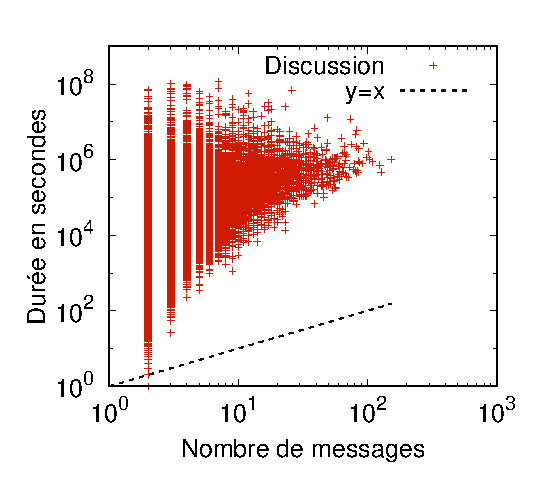
\includegraphics[width=\linewidth]{img/mailing/sizes-durations-corr.eps}
		\caption{\label{fig:corr_discussion_duration}}		
	\end{subfigure}
	\begin{subfigure}{0.4\textwidth}
		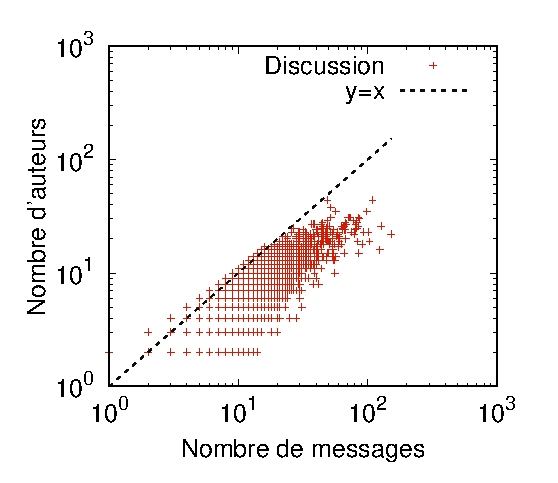
\includegraphics[width=\linewidth]{img/mailing/sizes-authors-corr.eps}
		\caption{\label{fig:corr_discussion_author}}
	\end{subfigure}

	\caption{En (A): Corrélation entre le nombre de courriels et la durée d'une discussion. En (B): Corrélation entre le nombre de courriels et le nombre de personnes dans une discussion.}
	\label{fig:corr_discussion}
\end{figure}

Comme attendu, nous observons dans la figure~\ref{fig:corr_discussion_duration} que plus une discussion est grande en nombre de courriels plus elle dure longtemps, ce qui est attendu.
Par contre, on observe que les petites discussions ont des durées très variables. 
Dans la figure~\ref{fig:corr_discussion_author} présentant la corrélation entre le nombre de courriels et celui de personnes, nous observons un autre fait attendu~\cite{dorat2007}: une discussion est constituée, en général, de plus de messages que de participants.
Ainsi lors d'une discussion, c'est un petit nombre de personnes qui échangent potentiellement beaucoup de messages. 

Enfin, il est intéressant d'observer la dynamique des échanges entre chaque paire de personnes.
Soit $\tau(u,v) = \{t_{i+1}-t_i\}_{i=0..k+1}$ la séquence des temps inter-contacts des $k$ liens entre les n\oe{}uds $u$ et $v$, où $t_0$ est le temps entre $\alpha$ et le premier lien et $t_{k+1}$ est le temps entre le dernier lien et $\omega$.
Il s'agit du temps écoulé avant que deux personnes se contactent à nouveau, peu importe la conversation.
Dans la figure~\ref{fig:ict_discussion} est représentée la distribution cumulative inverse du temps inter-contacts dans le flot de liens. 
On observe que $21\%$ des temps inter-contacts sont inférieurs à 30 jours ($2.6\times 10^6 s$).
Ce chiffre bien que relativement faible est tout de même important car il s'agit de discussions ouvertes où tout le monde peut participer. 
En particulier, une personne peut envoyer une demande d'aide à un moment donné et ne plus jamais échanger avec les même personnes.
Or, $21\%$ des contacts directs sont renouvelés en moins de 30 jours.
La participation est donc relativement élevée.
\begin{figure}
	\centering
	\includegraphics[width=0.4\linewidth]{img/mailing/ict-ccdf.eps}
	\caption{Distribution des temps inter-contacts dans le flot de liens.}
	\label{fig:ict_discussion}
\end{figure}

\section{\'Etude des discussions en tant que sous-flots}
\label{etude_discussion}
\subsection{Application de la \texorpdfstring{$\Delta$}{delta}-densité}
\label{delta_densite}

Jusqu'à maintenant aucune notion intrinsèquement liée aux flots de liens n'a été utilisée pour caractériser les discussions.
Le but est d'évaluer si cette structure de flot peut se rapprocher d'une structure communautaire.
Comme dit précédemment, les communautés sont souvent définies comme des structures devant être densément connectées.
C'est pourquoi nous nous attachons à étudier la densité des discussions.

Ces données se modélisent par un flot de liens où les liens n'ont pas de durée, nous étudions donc la densité non pas dans le flot de liens initial mais dans $\sigma(\xi(L,\Delta))$ pour différentes valeurs de $\Delta$ entre 1 seconde et 20 ans.
La notation $\delta{\alpha..\omega}(\sigma(\xi(L,\Delta)))$ est cependant très lourde et nous la simplifions par $\delta_{\Delta}(L)$ et nous parlons donc de $\Delta$-densité.
Tout d'abord dans la figure~\ref{fig:dens_fil_discusion} est représentée la $\Delta$-densité globale du le flot.
En couvrant un spectre aussi large de $\Delta$, on observe que la $\Delta$-densité est croissante avec $\Delta$ mais surtout on observe bien la convergence de $\Delta$-densité vers $3.139\times 10^{-4}$, la densité du graphe agrégé, lorsque $\Delta$ est proche de $\omega - \alpha$.

\begin{figure}[h]
	\centering
	\includegraphics[width=0.4\linewidth]{img/mailing/global_loglog.eps}
	\caption{Évolution de la $\Delta$-densité (en vert) du flot de liens pour $\Delta$ de $60$ seconde à $20$ ans. En rouge, la densité dans le graphe agrégé.}
	\label{fig:dens_fil_discusion}
\end{figure}

Cependant, la $\Delta$-densité du flot n'apporte que peu d'informations en elle-même.
Elle est surtout utile pour comparer les valeurs de $\Delta$-densité des sous-flots que sont les discussions, c'est-à-dire $\delta(\sigma(\xi(D_i,\Delta)))$.
Ainsi dans la figure~\ref{fig:intra_dens_discussion}, est présentée la distribution cumulative inverse de la $\Delta$-densité des discussions pour différentes valeurs de $\Delta$.
On remarque que les différentes valeurs de $\Delta$ ne semblent pas influencer qualitativement la distribution de $\Delta$-densité.
Cette courbe met surtout en évidence que les discussions sont des structures beaucoup plus denses que le flot.
En effet, la densité médiane des discussions varie, selon la valeur de $\Delta$, entre $2.69 \times 10^{-4}$ et $0.28$ alors que le flot a une $\Delta$-densité variant entre $1.05  \times 10^{-10}$ et $3.14 \times 10^{-4}$.
La $\Delta$-densité des discussions est donc en moyenne $10^{5}$ fois plus élevée que celle du flot.
Bien que notable, ce fait est attendu notamment car le flot dure beaucoup plus longtemps et concerne beaucoup plus de n\oe{}uds que les discussions.
\begin{figure}
\centering
%\subfloat[Inverse cumulative distribution of intra-threads density.]{
	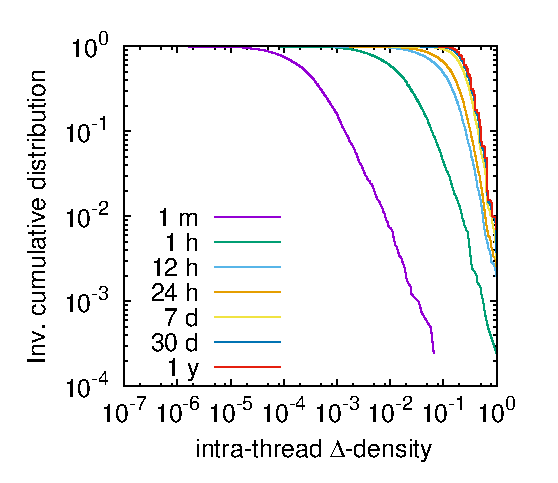
\includegraphics[width=0.4\linewidth]{img/mailing/delta.eps}
%}

\caption{Distribution cumulative inverse de la $\Delta$-densité des discussions pour différentes valeurs de $\Delta$.}
\label{fig:intra_dens_discussion}
\end{figure}

Afin d'aller plus loin dans l'étude de cette structure, il faut revenir à une définition plus précise de ce qu'est une bonne communauté.
En elle-même, une valeur de densité n'est pas suffisante pour définir une structure communautaire.
En effet, une discussion ayant une densité de $0.8$ peut ne pas être une communauté tandis qu'une autre ayant une densité proche de zéro peut être une communauté.
Il faut définir un point de comparaison pour effectivement affirmer qu'une structure est particulièrement dense.
La prise en compte de la densité globale est un début mais n'est pas suffisante.

Une autre définition d'une communauté est qu'elle devrait être plus densément connectée à l'intérieur qu'avec les autres communautés adjacentes.
Pour un graphe $G=(V,E)$ et une communauté $C_i$ de la partition $\mathcal{C} = \{C_j\}_{j_1..k}$ de $V$ en $k$ communautés, cela se traduit par le calcul de la densité entre les communautés, $\delta^{inter}(C_i)$ :

\begin{equation}
	\delta^{inter}(C_i) = \frac{1}{|C|-1}\sum_{j, i\ne j}\frac{|\{(u,v)\in E\mbox{ t.q. }u\in C_i\mbox{ et }v\in C_j\}|}{|C_i|\cdot |C_j|}.
\end{equation}
Il s'agit de la probabilité qu'un lien existe entre un n\oe{}ud de $C_i$ et un n\oe{}ud d'une autre communauté.
Encore une fois, cette notion n'a pas de sens direct dans le formalisme de flot de liens et il est nécessaire de l'adapter.
Pour ce faire, nous définissons la $\Delta$-densité inter-discussions entre deux discussions $D_i$ et $D_j$: $\delta^{inter}_{\Delta}(D_i,D_j)$.
Soient $\Delta_{ij}=\xi(D_i \cup D_j,\Delta)$ et $L_{inter}(D_i, D_j) = (T',V',E')$ avec:

\begin{itemize}
\item  $T'=[\beta(D_i \cup D_j) - \Delta/2,\psi(D_i \cup D_j) + \Delta/2]$, $V'= V(\Delta_{ij})$;
\item  $E' = \xi(E,\Delta) \setminus \Delta_{ij}$.
\end{itemize}
Avec ces notation, $\delta^{inter}_{\Delta}(D_i,D_j)$ est égale à:

\begin{equation}
 \delta^{inter}_{\Delta}(D_i,D_j) = \delta(L_{inter}(D_i, D_j))\, .
\end{equation}

Il s'agit donc de la densité du flot inter-discussions qui est constitué des liens entre les n\oe{}uds induits par $D_i$ et $D_j$ qui n'appartiennent ni à $D_i$ ni à $D_j$.
Dans la figure~\ref{fig:inter_dens_discussion_ex}, un exemple de flot inter-discussion est représenté.
Il est important de noter que le nombre de liens pris en compte dans le flot inter-discussions varie selon le $\Delta$ utilisé.

\begin{figure}
\centering
%\subfloat[Inverse cumulative distribution of inter-threads density.]{
	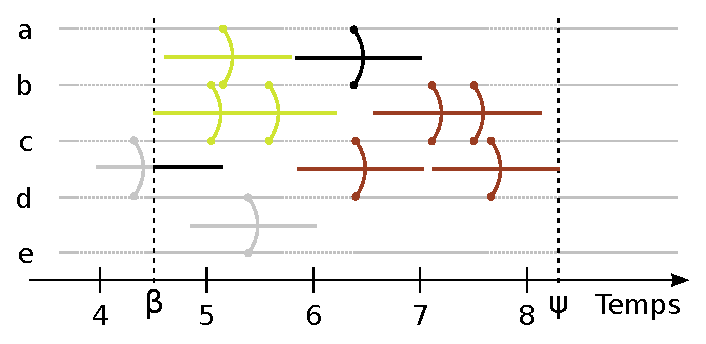
\includegraphics[width=0.65\linewidth]{img/mailing/inter_flot.eps}
%}
\caption{Exemple de flot inter-discussion.
Le flot entre les discussions \textcolor{olivegreen}{\textbf{verte}} et \textcolor{briquered}{\textbf{rouge}} est constitué des liens ou partie de liens en \textbf{noir}. Les liens en \textcolor{gray}{\textbf{gris}} ne sont pas pris en compte.}
\label{fig:inter_dens_discussion_ex}
\end{figure}



Afin d'obtenir la $\Delta$-densité inter-discussions entre $D_i$ et toutes les autres discussions, nous utilisons la moyenne des $\Delta$-densités inter-discussion entre $D_i$ et les autres discussions, soit:

\begin{equation}
	\delta^{inter}_{\Delta}(D_i) = \frac{1}{|C|-1}\sum_{j,i\ne j} \delta^{inter}_{\Delta}(D_i,D_j).
\end{equation}

La distribution cumulative inverse de la $\Delta$-densité inter-discussions est présentée dans la figure~\ref{fig:inter_dens_discussion} pour différentes valeurs de $\Delta$.
Bien que similaire, le comportement de la $\Delta$-densité inter-discussions diffère qualitativement de celui de la $\Delta$-densité.
La $\Delta$-densité inter-discussions croît aussi en fonction de $\Delta$ mais il y a toujours une différence notable entre $\Delta= 30\  jours$ et $\Delta= 1\ an$ ce qui n'est pas le cas pour la $\Delta$-densité.
Cette différence s'explique parce que quelque soit le $\Delta$, le nombre de liens considérés pour la $\Delta$-densité est fixe, au contraire, il croît avec $\Delta$ pour la $\Delta$-densité inter-discussion.
Cet effet est visible dans la figure~\ref{fig:inter_dens_discussion_ex}: le lien $(c,d)$ qui apparaît peu avant $\beta$ est en partie pris en compte, alors qu'il ne le serait pas avec un $\Delta$ plus proche de 0.

Un autre facteur est aussi la durée considérée qui est plus longue que la durée des discussions ce qui peut diminuer la densité.
\begin{figure}
\centering
%\subfloat[Inverse cumulative distribution of inter-threads density.]{
	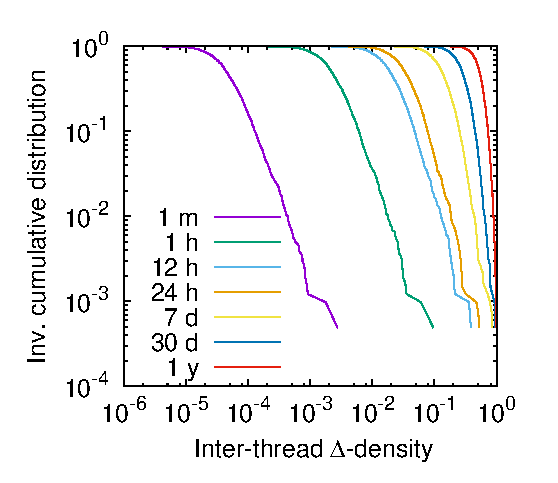
\includegraphics[width=0.4\linewidth]{img/mailing/inter_delta.eps}
%}
\caption{Distribution cumulative inverse de la $\Delta$-densité inter-discussions pour différentes valeurs de $\Delta$ en secondes.}
\label{fig:inter_dens_discussion}
\end{figure}

\bigskip

Pour comparer aisément $\Delta$-densité et $\Delta$-densité inter-discussions, nous présentons dans la figure~\ref{fig:corel_inter_discussion} la corrélation entre ces deux mesures pour différentes valeurs de $\Delta$.
Nous remarquons que les discussions sont effectivement plus denses intérieurement qu'avec les autres discussions.
La différence est de plusieurs ordres de grandeur lorsque $\Delta$ est petit et elle diminue lorsque $\Delta$ croît.
Pour $\Delta=20\ ans$ dans la figure~\ref{fig:corel_inter_discussion_20}, la différence n'est plus visible car à cette échelle de temps, l'ancrage temporel des discussions n'est plus décisif.
On remarque tout de même que pour $\Delta=1\ an$, la différence reste notable.
 

\begin{figure}[h]
\centering
	\begin{subfigure}{0.4\textwidth}
		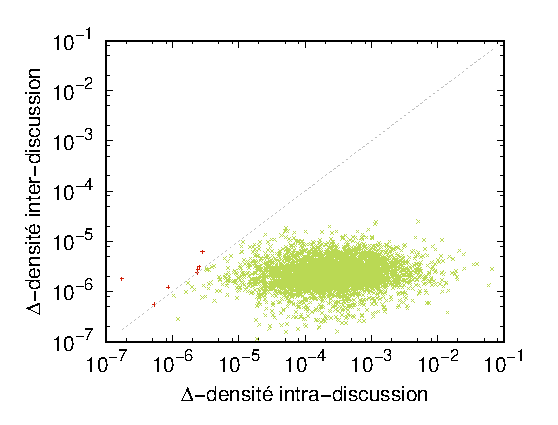
\includegraphics[width=\linewidth]{img/mailing/DensityCurve/120/mean.eps}
		\caption{$\Delta= $1 minute}		
	\end{subfigure}
	\begin{subfigure}{0.4\textwidth}
		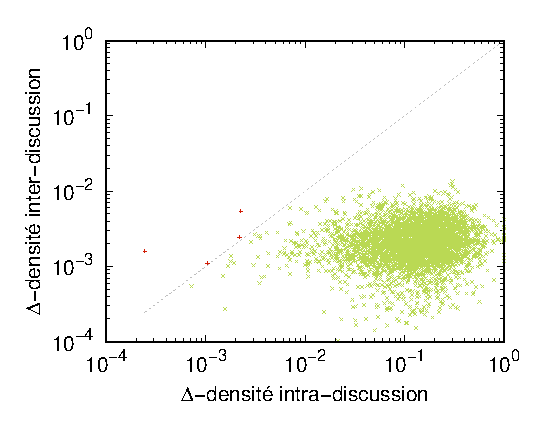
\includegraphics[width=\linewidth]{img/mailing/DensityCurve/172800/mean.eps}
		\caption{$\Delta= $1 jour}		
	\end{subfigure}
	
	\begin{subfigure}{0.4\textwidth}
		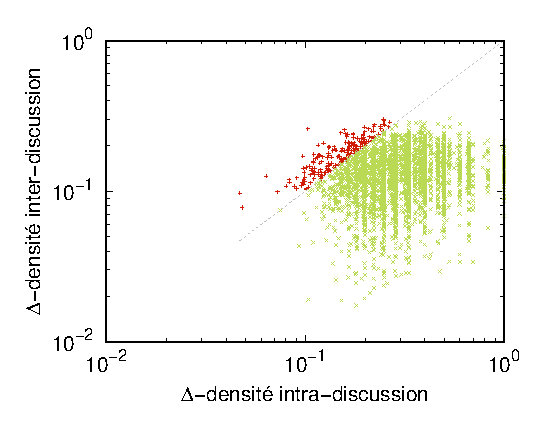
\includegraphics[width=\linewidth]{img/mailing/DensityCurve/63072000/mean.eps}
		\caption{$\Delta= $1 an}		
	\end{subfigure}
	\begin{subfigure}{0.4\textwidth}
		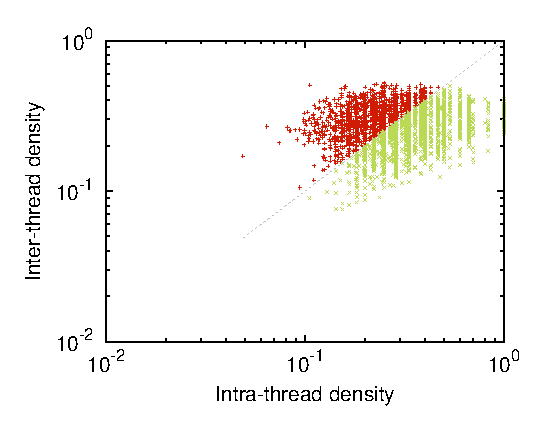
\includegraphics[width=\linewidth]{img/mailing/DensityCurve/1261440000/mean.eps}
		\caption{$\Delta= $20 ans}	
		\label{fig:corel_inter_discussion_20}	
	\end{subfigure}

\caption{Corrélations entre $\Delta$-densité et $\Delta$-densité inter-discussions pour différentes valeurs de $\Delta$. Une discussion est en vert (resp. rouge) si elle a une $\Delta$-densité plus (resp. moins) élevée que sa $\Delta$-densité inter-discussions.}
\label{fig:corel_inter_discussion}
\end{figure}



\subsection{Répartition temporelle et structurelle des discussions}

Nous avons étudié la densité interne aux discussions et entre les discussions mais il est également intéressant d'observer comment ces discussions sont réparties topologiquement et temporellement.
Pour étudier la répartition des discussions dans le temps, nous construisons un graphe d'intervalle~\cite{Lekkeikerker} $X=(V_X,E_X)$ représentant le chevauchement temporel.
Chaque discussion du flot devient un n\oe{}ud de $V_X$ et le lien $(i,j)$ existe dans $E_X$ si les discussions $D_i$ et $D_j$ correspondantes se recouvrent temporellement, \emph{i.e.} $[\alpha_i, \omega_i] \cap [\alpha_j, \omega_j] \neq \emptyset$.
De manière similaire, nous définissons le graphe de chevauchement topologique $Y=(V_Y,E_Y)$.
Les n\oe{}uds de ce graphe représentent encore une fois les discussions du flot et un lien existe entre deux discussions si au moins une personne a participé aux deux, \emph{i.e.} $V(D_i) \cap V(D_j) \neq \emptyset$.

Par construction, ces graphes contiennent beaucoup d'information sur les relations entre les discussions.
Ces deux graphes sont constitués de 116 999 n\oe{}uds et d'environ 2 millions de liens pour le graphe de chevauchement temporel et d'environ 63 millions de liens pour le graphe de chevauchement topologique.



Dans la figure~\ref{fig:x-y-graphs_discu_temp}, est représentée la corrélation entre le degré d'une discussion dans le graphe de chevauchement temporel $X$ et sa durée.
Il y a une corrélation évidente entre ces deux notions lorsque les discussions ont une durée supérieure à $10^5$ secondes.
Plus une discussion dure longtemps, plus elle a de chance d'avoir lieu en même temps que d'autres discussions.
Nous observons également que, même pour les discussions durant moins d'un jour ($8.6 \times 10^4$\,s), il peut y avoir jusqu'à une centaine d'autres discussions actives sur la même période.

\begin{figure}
\centering
	\begin{subfigure}{0.4\textwidth}
		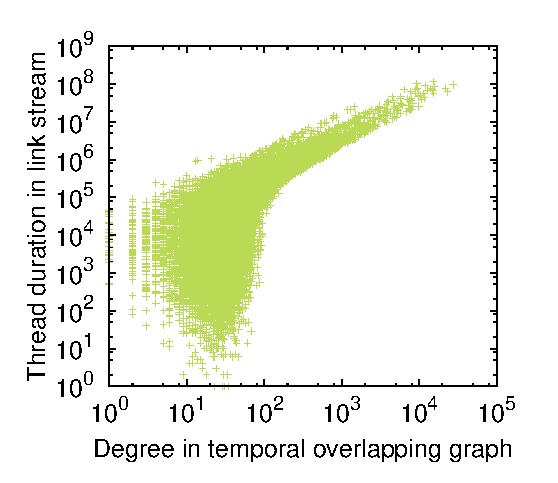
\includegraphics[width=\linewidth]{img/mailing/degree_temp}
		\caption{\label{fig:x-y-graphs_discu_temp}}		
	\end{subfigure}
	\begin{subfigure}{0.4\textwidth}
		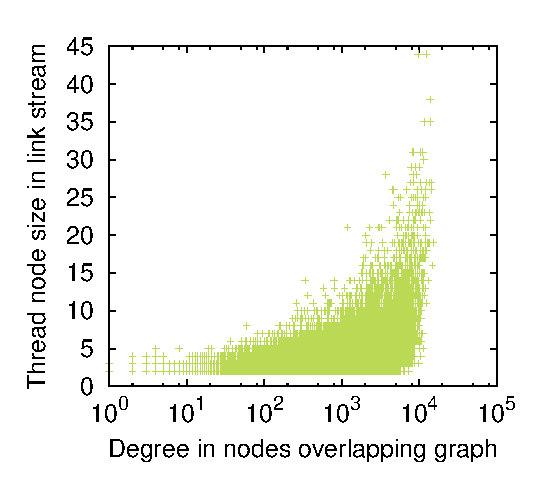
\includegraphics[width=\linewidth]{img/mailing/degree_nodes}
		\caption{\label{fig:x-y-graphs_discu_node}}	
	\end{subfigure}
	
	
	\caption{En (A): Corrélation entre le degré des discussions dans le graphe de chevauchement temporel et leur durée. En (B): Corrélation entre le degré des discussions dans le graphe de chevauchement topologique et leur nombre de participants.}
	\label{fig:x-y-graphs_discu}
\end{figure}

La figure~\ref{fig:x-y-graphs_discu_node}  présente la corrélation entre le degré d'une discussion dans le graphe de chevauchement topologique $Y$ et son nombre de participants.
La corrélation est moins nette mais il y a tout de même une tendance.
Par contre, nous remarquons de manière frappante que même une petite discussion peut partager des n\oe{}uds avec énormément d'autres discussions.


\subsection{Flot quotient}


Le graphe quotient, qui est équivalent au graphe de chevauchement topologique, est une autre notion clef pour étudier les relations entre les communautés d'un graphe $G=(V,E)$.
Soit une partition $C= \{C_i\}_{1 .. k}$ des n\oe{}uds de $G$ en $k$ communautés, chaque communauté est représentée dans le graphe quotient $\bar{G}$ par un n\oe{}ud dans $V$.
Il y a un lien entre deux communauté $C_i$ et $C_j$ dans $E$ s'il existe au moins un lien entre un n\oe{}ud de $C_i$ et un n\oe{}ud de $C_j$.
Voir une illustration sur la figure~\ref{fig:graph-quotient}.
Il est possible d'ajouter un poids sur les liens de $\bar{G}$ égal au nombre de liens reliant les communautés.
Le graphe quotient permet de facilement étudier, dans un graphe, les relations entre les communautés.

\begin{figure}
\centering
	\includegraphics[width=0.50\linewidth]{img/mailing/graph-quotient}
	\vfill
	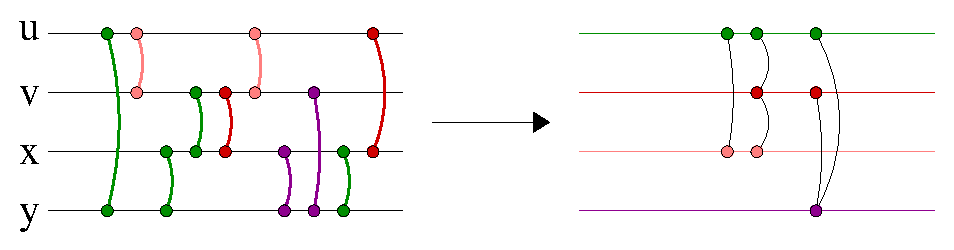
\includegraphics[width=0.75\linewidth]{img/mailing/stream-quotient}
	\caption{Haut: Exemple de graphe ayant une structure communautaire et son graphe quotient associé. Bas: Exemple d'un flot de lien avec une structure ainsi que son flot quotient associé.}
	\label{fig:graph-quotient}
%\label{fig:corel_inter}
\end{figure}

Nous étendons maintenant cette notion de graphe quotient aux flots de liens.
Nous définissons le flot quotient, $Q=(T_Q,V_Q,E_Q)$, induit par une partition $P=\{{P_i}\}_{1..k}$ en $k$ sous-flots de la manière suivante: chaque sous-flot $P_i$ est représenté par un n\oe{}ud dans $V_Q$.
Il existe un lien $(t_2,P_i,P_j)$ dans $E_Q$ s'il existe $(t_1,u,v) \in P_i$, $(t_2,u,v') \in P_j$ et $(t_3,u,v'') \in P_i$ avec $t_1 \leq t_2 \leq t_3$.
En d'autre termes, il y a un lien dans $E_Q$ si un n\oe{}ud $u$ a un lien dans $P_j$ qui apparaît entre deux autres de ses liens du groupe $P_i$.

Le flot quotient induit par les discussions dans le jeu de données contient $12\ 281\ 269$ liens impliquant $68\ 524$ discussions différentes.
Comme le jeu de données contient $116\ 999$ discussions, il y a donc $48\ 475$ discussions sans lien et qui ne seront pas prises en compte par la suite.
Ce nombre de discussions non-reliées est élevé comparé à ce qui pourrait être obtenu dans un graphe quotient.
En effet dans un graphe, un n\oe{}ud de degré $0$ correspond à une communauté qui est une composante connexe.
En ajoutant l'information temporelle, des discussions liées par leurs participants peuvent être séparées par le temps et les n\oe{}uds les représentant dans le flot ne seront alors pas liés.
Ce phénomène est d'autant plus vrai pour les discussions courtes.



Il faut aussi noter qu'il y a environ 20 fois plus de liens dans le flot quotient que dans le flot initial.
Cela s'explique par le fait qu'un lien dans le flot peut donner lieu à plusieurs liens dans le flot quotient.
Ce cas est visible dans la figure~\ref{fig:graph-quotient}. 
Le lien $(x,y)$ du groupe violet du flot à gauche donne lieu au lien $(\textcolor{plum}{violet}, \textcolor{red}{rouge})$ et au lien $(\textcolor{plum}{violet}, \textcolor{oliveGreen}{vert})$ dans le flot quotient à droite. 

\begin{figure}
\centering
	\includegraphics[width=0.4\linewidth]{img/mailing/quotient-density}
	\caption{$\Delta$-densité du flot de liens et du flot de liens quotient en fonction de $\Delta$ pour $\Delta=1mn, 1h, 12h, 1j, 7j, 30j, 1\ an$ et $20\ ans$.}
	\label{fig:quotient-stream-density}
\end{figure}

La figure~\ref{fig:quotient-stream-density} présente la $\Delta$-densité du flot de liens initial et du flot quotient pour différentes valeurs de $\Delta$.
Le flot initial et le flot quotient ont le même comportement de densité mais le flot quotient est moins $\Delta$-dense que le flot initial.
Ce résultat diffère de ce qui pourrait être obtenu avec un graphe quotient.
Cela est dû au nombre de n\oe{}uds qui est beaucoup plus important dans le flot quotient que dans le flot original, même si, le degré moyen dans le flot quotient est en moyenne 25 fois plus élevé que dans le flot original.


\section{Détection de structures denses}

\`A partir du constat que les discussions forment une structure particulière, il est naturel d'essayer de les retrouver automatiquement. 
Pour y parvenir, il faut un moyen capable de trouver des sous-flots denses dans le flot.
C'est à dire une méthode identifiant des groupes de liens qui soient proches temporellement et topologiquement.
Il serait tentant d'optimiser directement la densité dans le flot mais ce n'est pas envisageable car un groupe constitué d'un unique lien a une densité de $1$.
Il faut donc trouver une autre méthode.
C'est pourquoi nous avons construit une autre projection du flot en un graphe statique afin d'y appliquer une méthode de détection de communautés.
L'enjeu est alors de réussir à créer une transformation de telle sorte que les informations temporelles et topologiques ne soient pas complètement perdues.

\subsection{Méthode de détection}
\label{sec:fail_mailing}
Afin de créer une transformation du flot vers un graphe, nous définissons un autre flot de liens, $\mathfrak{L}$, dont les liens ont une durée.
\`A partir de $\mathfrak{L}$, nous créons un graphe non-orienté et non-pondéré $\mathcal{G} = (\mathcal{V},\mathcal{E})$. Nous commençons par décrire comment $\mathcal{G}$ est défini à partir de $\mathfrak{L}$.

Chaque un n\oe{}ud de $\mathcal{G}$ correspond à lien de $\mathfrak{L}$.
Deux liens $(b,e,u,v)$ et $(b',e',u',v')$ du flot de liens sont reliés dans $\mathcal{G}$ s'ils partagent un n\oe{}ud et si les intervalles s'intersectent, \emph{i.e.} $\{u,v\} \cap \{u',v'\} \neq \emptyset$ et $[b,e]\cap[b',e'] \neq \emptyset$ (voir la figure~\ref{fig:Transformation}).
Ainsi, un lien dans le graphe représente une connexion structurelle et temporelle entre deux liens du flot de liens.
Les groupes denses dans $\mathcal{G}$ représentent donc des groupes de liens connectés temporellement et topologiquement dans $\mathfrak{L}$.

\begin{figure}[h]
\centering
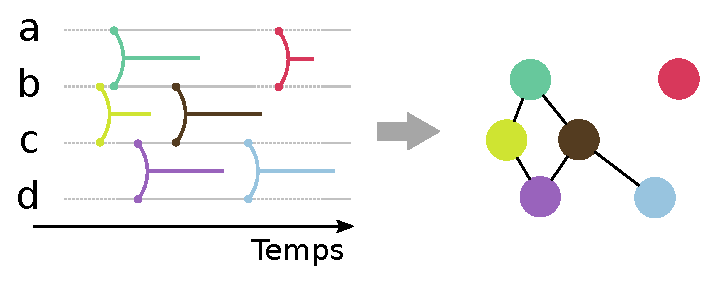
\includegraphics[width=0.55\linewidth]{img/mailing/Transformation.eps}
\caption{Transformation d'un flot de liens avec 4 n\oe{}uds (a-d) et 6 liens à gauche en un graphe à droite à 6 n\oe{}uds. La couleur d' un n\oe{}ud dans le graphe indique le lien du flot qu'il représente.}
\label{fig:Transformation}
\end{figure}%

Nous étudions maintenant comment ajouter une durée à chaque lien pour créer $\mathfrak{L}$.
Lors du calcul de la densité dans la section~\ref{delta_densite}, nous avions ajouté une durée arbitraire $\Delta$.
Ici, il n'est pas très pertinent d'appliquer la même logique.
En effet, si on utilise un $\Delta$ faible, alors il n'y aura que très peu de liens dans $\mathcal{G}$ et les n\oe{}uds représentant les liens d'une discussions ne seront pas forcément reliés.
Il parait illusoire d'espérer retrouver les discussions dans $\mathcal{G}$ si elles n'appartiennent pas à la même composante connexe.
Si $\Delta$ est très grand alors toute information temporelle est perdue et cela revient à calculer le \emph{line-graph}\,\footnote{Nous définissons le \emph{line-graph} dans le chapitre~\ref{chap:Expected_Node}.} du multigraphe agrégé.
C'est pourquoi nous adoptons une autre manière d'ajouter une durée sur les liens.

Pour chaque message $m$, nous connaissons $p(m)$, le message auquel il répond dans la discussion.
Nous définissons alors les liens de $\mathfrak{L}$ qui ont une durée de la manière suivante: ${(t(p(m)),t(m),a(m),a(p(m))}_m$.
Ainsi, deux messages $m_1$ et $m_2$ se succédant dans une discussion sont par définition reliés topologiquement car $a(m_1)= a(p(m_2))$.
Ces deux messages sont aussi reliés temporellement car nous avons la relation suivante:
\begin{align*}
[t(p(m_1)),t(m_1)]\cap [\mathbf{t(p(m_2))},t(m_2)] &= \\
[t(p(m_1)),t(m_1)]\cap [\mathbf{t(m_1)},t(m_2)] &= [t(m_1)] \neq \emptyset.
\end{align*}
Par construction, une discussion est donc représentée dans $\mathcal{G}$ par un ensemble connexe de n\oe{}uds.
Un fois $\mathcal{G}$ construit, on peut appliquer un algorithme de détection de communautés.

Avec cette construction, $\mathcal{G}$ contient plus d'1 millions de liens entre 316 569 n\oe{}uds pour les 116 999 discussions présentes.
Sur ce graphe, nous avons appliqué l'algorithme de Louvain~\cite{Blondel2008a} qui optimise la modularité.
D'autres algorithmes peuvent être appliqués s'ils détectent des groupes de n\oe{}uds disjoints et s'ils passent à l'échelle.
Les groupes trouvés par Louvain sont des communautés dans $\mathcal{G}$.
Par conséquent, ils sont censé être densément connectés dans $\mathcal{G}$.
Comme un lien de $\mathcal{G}$ correspond à une connexion temporelle et topologique dans le flot, on peut espérer qu'ils correspondent à des groupes denses dans le flot.
C'est ce que nous cherchons à montrer ensuite.

\subsection{Comparaison des partitions}

Avant de comparer la structure des discussions, $D$, et la partition, $\mathfrak{D}$, trouvée par la méthode de Louvain sur $\mathcal{G}$, il est nécessaire de décrire cette dernière.
Dans la figure~\ref{fig:carac_mail_louvain}, les distributions cumulatives inverses du nombre de liens, du nombre n\oe{}uds et de leur durée sont présentées pour les groupes de $\mathfrak{D}$.
Pour rappel, les même données sont représentées pour les discussions.
On remarque tout de suite que $\mathfrak{D}$ contient des groupes beaucoup plus gros en nombre de n\oe{}uds et de liens alors qu'ils ont des durées similaires.
\begin{figure}[h]
\centering
	\begin{subfigure}{0.4\textwidth}
		\includegraphics[width=\linewidth]{img/mailing/Detection/linksize}\hfill
		\caption{}		
	\end{subfigure}
	\begin{subfigure}{0.4\textwidth}
		\includegraphics[width=\linewidth]{img/mailing/Detection/nodeSize}\hfill
		\caption{}		
	\end{subfigure}

	\begin{subfigure}{0.4\textwidth}
		\includegraphics[width=\linewidth]{img/mailing/Detection/duree}\hfill
		\caption{}		
	\end{subfigure}
	\begin{subfigure}{0.4\textwidth}
		\includegraphics[width=\linewidth]{img/mailing/Detection/densite}
		\caption{\label{fig:dens_mail_louvain}}		
	\end{subfigure}
\caption{Distributions cumulatives inverses du nombre de liens (A), du nombre de n\oe{}uds (B), de la durée (C) et de la densité (D) pour les groupes trouvés par Louvain et les discussions.}
\label{fig:carac_mail_louvain}
\end{figure}



Ces deux structures sont donc très différentes mais cela pourrait être dû à l'algorithme de Louvain qui n'est pas adapté pour trouver des groupes denses.
C'est pourquoi nous avons également observé la densité des groupes de $D$ et $\mathfrak{D}$ dans le flot $\mathfrak{L}$.
Le résultat est visible dans la figure~\ref{fig:dens_mail_louvain}.
Comme les liens de $\mathfrak{L}$ ont une durée, il est possible d'utiliser directement la densité au lieu de la $\Delta$-densité utilisée précédemment.
On remarque que les groupes de $\mathfrak{D}$, bien que plus gros, sont plus denses que les groupes de $D$.
Cependant la distribution cumulative inverse cache les effets de la taille sur la densité.
Or, une analyse manuelle montre qu'à nombre de liens égal (entre $2$ et $160$) les groupes trouvés par Louvain sont plus denses en moyenne, $0.46$ contre $0.38$. 
La médiane est également légèrement plus élevée: $0.34$ contre $0.33$.
En revanche, les plus gros groupes ($\mathcal{D}_j|>160$) trouvés par Louvain ont une densité plus faible ce qui peut être dû à leur taille.

Si les groupes de $\mathfrak{D}$ sont plus denses, c'est peut-être car ils regroupent plusieurs discussions de $D$ dans un groupe.
Pour comparer deux partitions, l'indice de Jaccard est classiquement utilisé pour calculer la précision et le rappel qui sont définis de la manière suivante:

\begin{equation*}
pr\acute{e}cision(\mathfrak{D}_j)= \max_{i} \frac{|\mathfrak{D}_j \cap D_i|}{|\mathfrak{D}_j|}\,, \quad \qquad
rappel(D_i)= \max_{j} \frac{|\mathfrak{D}_j \cap D_i|}{|D_i|}.
\label{eq:rappel}
\end{equation*}

Dans la figure~\ref{fig:rec_inclusion_niveau0}, sont présentées la précision des groupes capturés et le rappel des discussions en fonctions de leur taille.
Chaque point représente la moyenne de la précision (resp. rappel) pour les groupes (resp. discussions) d'une taille donnée.
On voit qu'il y a un important rappel et ce même pour les grandes discussions, ce qui veut dire qu'en général une discussion $D_i$ est totalement incluse dans un groupe $\mathfrak{D}_j$.
En revanche, la précision est très faible car un groupe $\mathfrak{D}_j$ contient plusieurs discussions, ce qui est cohérent avec la taille très importante des groupes de $\mathfrak{D}_j$.

\begin{figure}
\centering

\hfill
	\begin{subfigure}{0.45\textwidth}
		\includegraphics[width=\linewidth]{img/mailing/Detection/Rappel_0.eps}
		\caption{}		
	\end{subfigure}\hfill
	\begin{subfigure}{0.45\textwidth}
		\includegraphics[width=\linewidth]{img/mailing/Detection/Precision_0.eps}
		\caption{}		
	\end{subfigure}\hfill

\caption{(A) Rappel des discussions vis-à-vis des groupes trouvés par Louvain.
 (B) Précision des groupes trouvés vis-à-vis des discussions.
Chaque point représente la moyenne du rappel (resp. précision) pour les discussions (resp. groupes) ayant la même taille.
La couleur du point indique le nombre de groupes ayant la même taille.}
\label{fig:rec_inclusion_niveau0}
\end{figure}


Il semble donc que la partition $\mathfrak{D}$ soit proche de $D$ mais que ses groupes soient plus gros.
Pour circonvenir à ce problème, nous appliquons de manière récursive l'algorithme de Louvain sur chaque graphe induit par un groupe $\mathfrak{D}_j$.
Ce processus permet de subdiviser chaque groupe $\mathfrak{D}_j$.
Le niveau $0$ est la première partition trouvée par l'algorithme de Louvain dans $\mathcal{G}$, c'est-à-dire $\mathfrak{D}_{0,j}=\mathfrak{D}_j$.
Soit $\mathfrak{D}_{h,j'}$ un groupe trouvé au niveau $h$, par construction, il est inclus dans un groupe trouvé au niveau $h-1$, c'est à dire $\mathfrak{D}_{h,j'} \subseteq \mathfrak{D}_{h-1,j}$.


Soit $D_i \in D$, notons $\mathfrak{D}_{h,\tilde{i}}$ le groupe trouvé par la méthode de Louvain au niveau $h$ qui soit le plus proche de $D_i$, c'est-à-dire $|\mathfrak{D}_{h,\tilde{i}}\cap D_i|= \max_{j} |\mathfrak{D}_{h,j} \cap D_i|$.
Avec ces définitions, on observe la relation suivante: $\mathfrak{D}_{h,\tilde{i}}\cap D_i \subseteq \mathfrak{D}_{h-1,\tilde{i}}\cap D_i$.
La définition de rappel de l'équation~\ref{eq:rappel} n'est donc pas adaptée pour les niveaux inférieurs et nous l'adaptons de la manière suivante:

\begin{equation}
rappel(D_i,h)= \max_{j} \frac{|\mathfrak{D}_{h,j} \cap D_i|}{|D_i \cap \mathfrak{D}_{h-1,\tilde{j}}|}.
\end{equation}

Ainsi, le rappel au niveau $h$ prend en compte le maximum d'élément qu'il est possible de trouver à ce niveau.
La définition de précision ne pose quant à elle pas de problème.
La figure~\ref{fig:rec_inclusion} représente le rappel adapté et la précision pour le premier et deuxième niveau de récursion de la même manière que pour la figure~\ref{fig:rec_inclusion_niveau0}.
On remarque que, dès le premier niveau, le rappel baisse et que ce phénomène s'amplifie fortement au niveau suivant.
Cela implique que les discussions ne sont plus incluses dans un groupe mais au contraire réparties dans plusieurs.
La précision quant à elle augmente légèrement mais cela est dû à la baisse de la taille des groupes trouvés.
Il semble donc qu'il ne soit pas possible avec cette approche de retrouver automatiquement les discussions.


\begin{figure} [h]
\centering

	\begin{subfigure}{0.45\textwidth}
		\includegraphics[width=\linewidth]{img/mailing/Detection/Rappel_1.eps}
		\caption{niveau 1}		
	\end{subfigure}
	\begin{subfigure}{0.45\textwidth}
		\includegraphics[width=\linewidth]{img/mailing/Detection/Precision_1.eps}
		\caption{niveau 1}		
	\end{subfigure}
	
	\begin{subfigure}{0.45\textwidth}
		\includegraphics[width=\linewidth]{img/mailing/Detection/Rappel_2.eps}
		\caption{niveau 2}		
	\end{subfigure}
	\begin{subfigure}{0.45\textwidth}
		\includegraphics[width=\linewidth]{img/mailing/Detection/Precision_2.eps}
		\caption{niveau 2}		
	\end{subfigure}

\caption{(A,C) Rappel des discussions vis-à-vis des groupes trouvés par Louvain à différent niveaux récursifs.
(B,D) Précision des groupes trouvés vis-à-vis des discussions.
Chaque point représente la moyenne du rappel (resp. précision) pour les discussions (resp. groupes) ayant la même taille.
La couleur du point indique le nombre de groupes ayant la même taille.
}
\label{fig:rec_inclusion}
\end{figure}

\subsection{Conclusion et perspectives}

\subsubsection{Conclusion}

Nous avons utilisé le modèle de flot de liens pour étudier une archive de courriels provenant du projet Debian.
Grâce au modèle de flot de liens, nous avons proposé des notions clefs pour mieux comprendre la répartition temporelle et topologique des discussions.
Nous avons notamment étudié la notion de $\Delta$-densité sur les discussions en elles mêmes.
Puis, nous avons étudié les relations entre les discussions avec la $\Delta$-densité inter-discussions, les projections en graphes de chevauchement temporel ou topologique et le flot quotient.

Cette étude repose en grande partie sur la notion de $\Delta$-densité qui nécessite de fixer arbitrairement $\Delta$.
Nous avons à chaque fois testé un ensemble de valeurs de $\Delta$ variant d'une seconde jusqu'à parfois 20 ans et, lors de ces tests, aucune valeur $\Delta$ caractéristique n'a pu être identifiée.
La $\Delta$-densité est donc relativement robuste vis-à-vis de $\Delta$ dans ce jeu de données.

Ces métriques nous ont permis d'observer que les discussions forment une structure plus dense que le flot de liens.
De manière encore plus forte, nous avons constaté, grâce à la $\Delta$-densité inter-discussion, que les discussions sont plus denses en interne qu'en externe.
C'est une caractéristique importante des communautés que l'on trouve dans les graphes mais qui n'avait pas encore été observée dans un contexte temporel.
Forts de ces découvertes, nous avons poursuivi la recherche par l'étude des relations à un niveau plus macro: celles entre les discussions.
Via le graphe de chevauchement temporel, nous avons validé le fait que différentes discussions ont lieu en même temps et que par conséquent une agrégation temporelle entraînerait une perte d'information.
De même via le graphe de chevauchement topologique, nous avons mis en évidence une structure très recouvrante sur les n\oe{}uds, rendant l'utilisation de partitions statiques de n\oe{}uds difficilement envisageable pour décrire les discussions.


Par la suite, nous avons mis en place un première méthode de détection de partition de liens.
Cette méthode se base sur la projection du flot de liens en un graphe statique sur lequel nous appliquons un algorithme de détection de communautés provenant de la théorie des graphes.
Nous avons, avec cette méthode, mis en évidence des groupes denses.
Les groupes trouvés sont plus gros et plus denses que la structure des discussions mais les incluant.
Il semble donc qu'il existe une autre structure pertinente que celle des discussions et il serait intéressant de mettre au jour son sens.

Ces observations ne remettent d'ailleurs pas en cause les conclusions faites sur les discussions, pour plusieurs raisons.
Tout d'abord, les flots de liens étudiés ne sont pas exactement les-mêmes ($L\neq \mathfrak{L}$).
Ce changement de flot est nécessaire pour le fonctionnement de la méthode de détection mais cela change l'objet d'étude.
Ensuite, les deux structures ne sont pas complètement différentes car les groupes trouvés semblent en fait agréger plusieurs discussions.
Malheureusement, nous n'avons pas réussi avec notre méthode à isoler chaque discussion malgré notre approche récursive.
Pourtant, il semble que la structure trouvée ait du sens au vu des valeurs de densité des groupes.

\subsubsection{Perspectives}

Ce jeux de données de courriels est intéressant.
D'une part, il couvre une très longue période de temps et, d'autre part, il existe de nombreuses informations associées.
Nous avons utilisé ici la connaissance de la discussion associée à chaque courriel pour étudier la notion de communautés.
D'autres notions pourraient être développées grâce sur ce jeu de données, notamment les notions de centralité et de rôle des n\oe{}uds.
Grâce à la durée de presque $20$ ans du jeu de données, il serait intéressant de mesurer l'évolution de l'implication et du rôle d'une personne.
Il serait ainsi possible de mieux comprendre la participation de personnes à un projet de cette ampleur.

Il y a également le texte brut du mail qui est accessible et dont nous n'avons pas tiré parti.
Il serait sûrement intéressant pour des linguistes de quantifier l'évolution du vocabulaire.
De même, nous nous sommes focalisés sur la liste de discussion anglaise, alors qu'il est possible avec le script d'extraction de considérer les listes de discussions dans d'autres langues.
Il pourrait être intéressant de comparer les structures obtenues pour différentes langues.

\bigskip



Lors la manipulation de flot de liens, un enjeu important est la compréhension de la structure de liens que nous avons détectée.
C'est cette perspective que nous poursuivons dans le chapitre suivant.



\chapter{Détection de groupes pertinents dans les flots de liens}
\minitoc

\label{groupesDense}
Nous avons vu précédemment qu'il est possible de trouver des groupes de liens dans un flot de liens via l'intermédiaire d'une projection du flot de liens en un graphe statique.
Pour ce faire, nous avons appliqué l'algorithme de Louvain sur la projection pour obtenir une partition des liens en communautés.
Parmi l'ensemble des communautés, il se peut que certaines identifient des structures plus importantes et plus pertinentes que d'autres.
Le but est de réussir à extraire parmi ces groupes ceux qui sont pertinents.
Nous nous posons la question de la décomposition partielle d'un flot de liens en sous-flots pertinents.
Il s'agit d'un problème légèrement différent de la détection de partition car d'une part, certains liens peuvent n'appartenir à aucun groupe et, d'autre part, les groupes doivent être pertinents.

Toute la difficulté, pour trouver les groupes pertinents, est de réussir à mesurer la pertinence d'un groupe.
La notion de densité utilisée précédemment est une première approche mais ce n'est pas suffisant.
En effet, il peut exister de grands groupes pertinents mais peu denses et de petits groupes très denses mais peu pertinents.
Il n'est pas possible de faire la différence entre ces deux catégories en utilisant uniquement la densité.
C'est pourquoi, nous utilisons la notion de voisinage: un groupe est pertinent s'il est plus dense que son voisinage.
Par exemple, un groupe ayant une densité de $0.4$ est très pertinent dans un flot de liens ayant une densité globale de $0.01$, mais il ne l'est pas du tout si le flot de liens a une densité de $0.6$.
Comme le but est de pouvoir décrire le flot de liens, nous nous limitons aux groupes ayant une taille supérieure à un minimum donné.
Un exemple de flot avec une décomposition en groupes pertinents est présenté dans la figure~\ref{fig:exemple_groupe_dens}.

Afin de trouver des groupes pertinents, nous procédons de la manière suivante:
\begin{itemize}
\item nous construisons la projection du flot de liens en un graphe statique;
\item nous appliquons sur cette projection un algorithme de détection de communautés afin d'obtenir une partition des liens du flot de liens;
\item nous ne gardons dans la partition que les groupes qui sont considérés comme pertinents, c'est-à-dire ceux qui sont assez gros et qui sont plus denses que leur voisinage.
\end{itemize}

Afin de montrer la pertinence de cette approche, nous l'appliquons sur différents jeux de données et faisons une analyse manuelle de certains groupes trouvés.
Par ailleurs, nous montrons que les groupes que nous détectons ne peuvent pas être obtenus par une méthode statique.

Le chapitre est organisé de la manière suivante:
dans la section~\ref{sec:groupe_dense_existant}, nous revenons sur les travaux existants qui traitent de sujets similaires.
Puis dans la section~\ref{sec:groupe_dense_method}, nous présentons notre méthode de détection et de validation de groupes pertinents.
Enfin, nous présentons les jeux de données utilisés dans la section~\ref{sec:groupe_dense_result} et les résultats associés dans la section~\ref{sec:groupe_dense_data}.

\begin{figure}
\centering
\includegraphics[width=\linewidth]{img/GroupeDense/GroupExample/Zone_dense.eps}
\caption{Exemple de flots de liens avec 3 groupes denses représentés par la couleur des liens (\textcolor{brique}{\textbf{rouge}}, \textcolor{vert_turquoise}{\textbf{vert}} et \textcolor{bleu_window}{\textbf{bleu}}).
}
\label{fig:exemple_groupe_dens}
\end{figure}

\section{Travaux existants}
\label{sec:groupe_dense_existant}

Comme nous l'avons vu dans le chapitre~\ref{chap:etat_art}, il existe peu de méthodes cherchant des structures dans un formalisme sans perte d'information.

Mitra \emph{et al.}~\cite{Mitra2012a} et Speidel \emph{et al.}~\cite{Speidel2015} ont proposé des méthodes de détection de communautés dans les réseaux diachroniques.
Dans un tel réseau, ce sont les n\oe{}uds qui sont datés et non les liens.
Ce cas de figure s'applique parfaitement aux réseaux de citations car une citation relie bien deux publications apparues à deux dates spécifiques.
Cependant, ce genre de situation ne peut pas être simplement représenté par le formalisme de flot de liens.
C'est pourquoi nous ne pouvons utiliser la même méthode. 

Il existe des méthodes identifiant la partie la plus dense d'un réseau.
C'est le cas de Bogdanov \emph{et al.}~\cite{Bogdanov2011} qui considèrent un graphe dont la topologie n'évolue pas mais dont les poids des liens changent entre $-1$ et $1$ en fonction du temps.
Ce formalisme est aussi très différent de celui de flot de liens.
De plus, la notion de densité utilisée ne tient pas vraiment compte du temps car un groupe de n\oe{}uds sur un intervalle est évalué par la somme des liens entre ces n\oe{}uds sur tout l'intervalle.


Epasto \emph{et al.}~\cite{Epasto2015} détectent le sous-graphe le plus dense dans un graphe temporel.
Ainsi, le temps est bien pris en compte dans le formalisme.
Cependant, la méthode identifie le sous-graphe à un instant $t$ tel qu'il ait le degré moyen le plus élevé parmi l'ensemble des sous-graphes sur tous les instants.
Cette notion de densité est statique car elle ne considère que la structure de graphe à un instant.


Les travaux de Rozenshtein \emph{et al.}~\cite{rozenshtein2014} sont ceux qui se rapprochent le plus de notre méthode.
Leur méthode utilise le formalisme de flots de liens et ne suppose pas de structure de graphe à un instant donné.
Elle détecte un groupe de n\oe{}uds et plusieurs intervalles disjoints de telle sorte que ce groupe de n\oe{}uds dans le graphe agrégé sur ces intervalles ait le degré moyen le plus élevé.
Plus formellement, un groupe de n\oe{}uds $V'\subset V$ et un ensemble d'intervalles $\{I_1,..,I_k\} = \mathcal{I} \subset T$ doivent maximiser $\tilde{d}_\mathcal{G}(V')$ où $\mathcal{G}= \bigcup G(L_t),\,\forall t \in \mathcal{I}$.
Ainsi, même si la méthode permet d'identifier un groupe de n\oe{}uds sur des intervalles de temps, elle évalue un candidat sur un graphe agrégé pour appliquer une métrique de graphe.
Le temps n'a donc une influence qu'indirecte sur l'évaluation.
Par ailleurs, leur méthode repose sur plusieurs paramètres qui doivent être fixés \emph{a priori}: le nombre maximal d'intervalles disjoints et la durée cumulée maximale de ces intervalles.
Le premier paramètre permet d'éviter d'utiliser une infinité d'intervalles qui seraient chacun centré sur un lien.
Le second paramètre permet d'éviter de considérer tout le graphe agrégé et ainsi d'imposer la prise en compte du temps.
Ainsi, leur méthode dépend de manière non évidente du choix des paramètres.

Enfin, des travaux conduits dans l'équipe~\cite{viard:hal-01208330,Viard2016} ont étudié la détection de delta-cliques dans les flots de liens sans durée, c'est à dire dans un ensemble de $(b,b,u,v)$.
Pour un delta donné, une delta-clique est un ensemble de n\oe{}uds et un intervalle de temps, tels que toutes les paires de n\oe{}uds dans cet ensemble interagissent au moins tous les delta sur cet intervalle.
Cela est équivalent à trouver des ensembles de n\oe{}uds sur un intervalle de temps ayant une densité égal à $1$ dans le flot de liens où chaque lien a une durée delta\,\footnote{Un lien $(b,b,u,v)$ doit être transformé en $(b-\Delta,b,u,v)$.}.
Leur méthode est donc très proche mais elle ne détecte que des groupes de densité $1$ et ne prend pas en compte leurs voisinages.


\bigskip

\resume{il existe des méthodes cherchant la structure la plus dense dans un contexte dynamique; soit en considérant un graphe temporel soit en considérant un flot de liens.
Cependant, ces méthodes utilisent des métriques de graphe pour évaluer un groupe de n\oe{}uds.
Le temps n'est donc pas complètement pris en compte dans l'évaluation.
De manière plus importante, ces méthodes évaluent de manière absolue un groupe sans prendre en compte son voisinage.
Enfin, nous identifions plusieurs groupes de liens alors que les autres méthodes détectent un groupe n\oe{}uds.
Certaines de ces méthodes peuvent être étendues pour identifier les $k$ groupes de n\oe{}uds les plus denses mais cela se fait au prix de l'ajout d'un paramètre pour contrôler le chevauchement entre deux groupes.
}


\section{Détection de groupes pertinents}
\label{sec:groupe_dense_method}

Nous avons défini dans le chapitre précédent~\ref{sec:fail_mailing} une projection du flot de liens en un graphe statique.
Dans cette projection, chaque lien du flot est représenté par un n\oe{}ud.
Deux liens $(b,e,u,v)$ et $(b',e',u',v') \in L$ sont reliés dans le graphe s'ils partagent un n\oe{}ud et si les intervalles s'intersectent, \emph{i.e.} $\{u,v\} \cap \{u',v'\} \neq \emptyset$ et $[b,e]\cap[b',e'] \neq \emptyset$ (voir la figure~\ref{fig:Transformation}).
Sur cette projection, nous appliquons l'algorithme de Louvain pour la détection de communautés.
Les communautés trouvées par l'algorithme sont des groupes potentiellement pertinents et nous les appelons donc groupes "candidats".

Tous les groupes candidats ne sont pas forcément pertinents.
Tout d'abord, les groupes d'une partition peuvent avoir des tailles très variées.
En particulier, il peut y avoir beaucoup de très petits groupes de $1$ ou $2$ liens.
Ces groupes ne sont pas pris en compte car nous fixons \emph{a priori} une taille minimum des groupes fixée.

Par ailleurs, l'algorithme de Louvain optimise de manière gloutonne la modularité dans la projection du flot de liens en un graphe statique et non une métrique de flot de liens directement.
C'est pourquoi certains candidats peuvent être une bonne communauté dans le graphe mais un groupe non pertinent dans le flot de liens.
Ce phénomène est d'autant plus important que la modularité ne prend pas en compte le voisinage d'un groupe.
Par exemple, dans la figure~\ref{fig:exemple_groupe_dens}, les liens dans l'intervalle $[4,8]$ forment une composante connexe dans la projection et ils sont considérés comme une communauté par l'algorithme de Louvain.
Or, ces liens ne sont pas un groupe pertinent car ils sont beaucoup moins denses que les liens durant l'intervalle $[0,4]$ ou l'intervalle $[7,11]$.
C'est pourquoi il est nécessaire de filtrer les groupes candidats pour ne garder que les groupes pertinents.




\subsection{Définition des voisinages}
Dans le chapitre~\ref{sec:def_densite}, nous avons défini la densité d'un flot de liens.
Pour un groupe de liens, il faut donc calculer la densité du sous-flot induit par ses liens.
La densité en elle même n'est pas un bon critère pour évaluer la pertinence d'un candidat car un candidat constitué d'un unique lien a une densité maximale de $1$.
C'est pourquoi, il est nécessaire de tenir compte du voisinage.
Ainsi, plus le candidat a une densité plus supérieure à son voisinage, plus le candidat est un groupe pertinent.

Il est nécessaire de définir une notion de voisinage qui puisse tenir compte à la fois de la structure et du temps.
Pour ce faire, il faut utiliser une autre formulation de la densité pour comprendre quels sont les paramètres qui influent sur la densité.
Jusqu'à maintenant pour un candidat $C_i$, nous considérions la densité du sous-flot induit par ses liens, $\delta(L(C_i))$.
Pour faire apparaître l'influence de la structure et du temps, nous utilisons $\delta(L_{\beta(C_i)..\psi(C_i)}(V(C_i)^2))$ que nous notons, par abus de notation, $\delta(V(C_i),\beta(C_i), \bar{C_i})$ où $\bar{C_i} = \psi(C_i)-\beta(C_i)$.
Il s'agit de la densité des n\oe{}uds induits par $C_i$ sur la durée du groupe.
Ces deux quantités ne sont pas complètement équivalentes car les deux sous-flots sont différents, en particulier $L(C_i) \subseteq L_{\beta(C_i)..\psi(C_i)}(V(C_i)^2)$.
De cette inclusion découle le fait que $\delta(L(C_i)) \leq \delta(V(C_i),\beta(C_i), \bar{C_i})$.
C'est le cas dans l'exemple de la figure~\ref{fig:exemple_groupe_dens} si l'on calcule la densité des liens noirs.
Dans ce cas, tous les n\oe{}uds sont induits par ces liens et l'intervalle de temps est égal à $[2,11]$.
Le sous-flot induit par $V$ sur $[2,11]$ comprend l'ensemble des liens noirs mais aussi des liens \textcolor{vert_turquoise}{\textbf{verts}} et \textcolor{bleu_window}{\textbf{bleus}}.


Cependant avec cette formulation, on fait aussi apparaître 3 dimensions: l'ensemble de n\oe{}uds, le temps de début et la durée.
Il devient alors aisé de considérer comme voisins les sous-flots qui diffèrent sur une seule dimension: soit le temps de début, soit la durée soit l'ensemble de n\oe{}uds.
Cette différence entre les voisinages est illustrée dans la figure~\ref{fig:voisinage_groupe}.

\begin{figure}
\centering
	\begin{subfigure}{0.31\textwidth}
		\includegraphics[height=3cm]{img/GroupeDense/GroupExample/Voisinage/Base.eps}
		\caption{Groupe de liens initial}
	\end{subfigure}\hspace*{0.05cm}

	\begin{subfigure}{0.32\textwidth}
		\includegraphics[height=3cm]{img/GroupeDense/GroupExample/Voisinage/Variable_Nodes.eps}
		\caption{Voisinage sur les n\oe{}uds}
	\end{subfigure}
	\begin{subfigure}{0.32\textwidth}
		\includegraphics[height=3cm]{img/GroupeDense/GroupExample/Voisinage/Variable_duration.eps}
		\caption{Voisinage sur la durée}
	\end{subfigure}
	\begin{subfigure}{0.32\textwidth}
		\includegraphics[height=3cm]{img/GroupeDense/GroupExample/Voisinage/Variable_start.eps}
		\caption{Voisinage sur le temps de début}
	\end{subfigure}	
	\caption{Exemple d'un groupe de liens en (A) et de ses différents voisinages en (B), (C) et (D).
	La zone en \textcolor{bleu_transparent}{\textbf{bleu}} est la zone prise en compte lors du calcul de la densité.
	La zone en pointillé représente la zone considérée lors du calcul de la densité du groupe initial.
	}
	\label{fig:voisinage_groupe}
\end{figure}


Pour le voisinage aux n\oe{}uds, il est impossible de considérer l'ensemble de tous les ensembles de n\oe{}uds car il est beaucoup trop grand.
De plus, il est probable que ces groupes de n\oe{}uds ne soient même pas connexes dans le graphe agrégé si le flot de liens est peu dense.
C'est pourquoi si $V(C_i)$ est constitué de $k$ n\oe{}uds, nous nous limitons à l'ensemble des groupes de $k$ n\oe{}uds qui partagent $k-1$ n\oe{}uds avec $V(C_i)$.
De cette manière, on considère uniquement des groupes de n\oe{}uds similaires au candidat.
Cette comparaison nous semble plus stricte mais plus équitable que celles qui utilise l'ensemble des groupes de n\oe{}uds ou des groupes de n\oe{}uds pris aléatoirement.
Il serait possible de considérer un nombre moins important de n\oe{}uds partagés mais nous ne l'avons pas fait à cause de la complexité de calcul.
En effet, il y a déjà $k(|V|-k)$ sous-flots partageant $k-1$ n\oe{}uds avec un candidat.

Pour le voisinage au temps de début (resp. à la durée), nous considérons toutes les valeurs possibles de temps de début (resp. durée) dans un intervalle donné.
Chacune de ces valeurs donne lieu à un sous-flot induit ayant les mêmes n\oe{}uds et la même durée (resp. temps de début) que le sous-flot induit par les liens du groupe candidat.
Ensuite, nous calculons la densité de chacun de ces sous-flots voisins.
L'ensemble des densités des sous-flots voisins se définit de la manière suivante.
Soit $I_{d\acute{e}but}$ et $I_{dur\acute{e}e}$, deux intervalles représentant respectivement les valeurs de temps de début et de durée que nous allons considérer et $C_i$, un groupe de liens.
Les densités des sous-flots dans le voisinage au temps de début sont définies par la fonction $\delta(V(C_i),x, \bar{C_i})$, $\forall x \in I_{d\acute{e}but}$.
Les densités des sous-flots dans le voisinage de la durée sont définies par la fonction $\delta(V(C_i),\beta(C_i), y)$, $\forall y \in I_{dur\acute{e}e}$.

L'intervalle utilisé pour le voisinage au temps de début est $I_{d\acute{e}but}=[\alpha, \omega-\bar{C_i}]$.
L'intervalle utilisé pour le voisinage à la durée est $I_{dur\acute{e}e}=[0.8\Delta_{min}, 1.2\Delta_{max}]$, où $\Delta_{min}$ (resp. $\Delta_{max}$) est la plus petite (resp. grande) durée de tous les candidats de plus de 10 liens.
Nous utilisons cet intervalle pour deux raisons.
Tout d'abord, il contient l'ensemble des durées acceptables quand nous l'appliquons à nos jeux de données.
Mais surtout, nous avons testé l'intervalle $[1,\omega-\alpha]$ qui est beaucoup plus grand.
Cela change les résultat de manière quantitative mais pas de manière qualitative.
En effet lorsque la durée considérée est proche de $\omega-\alpha$, alors la densité est très proche de $0$.
Comme ces valeurs sont peu informatives, nous préférons nous limiter à un intervalle de durée plus restreint.
\bigskip

Au final, nous recherchons pour chaque voisinage les valeurs de densités des sous-flots voisins.
Pour le voisinage aux n\oe{}uds, il y a $k(|V|-k)$ valeurs de densité différentes.
Pour le voisinage au temps de début (resp. à la durée), nous avons une fonction de la densité qui dépend du temps de début (resp. de la durée).


\subsection{Définition de l'évaluation}
Nous évaluons chaque groupe candidat en comparant sa densité à celle des sous-flots dans chaque voisinage.
Si un candidat est vraiment pertinent, alors il devrait avoir une densité significativement plus élevée que la plupart des sous-flots voisins.
Si les densités des sous-flots voisins suivaient une distribution connue, par exemple une loi normale, cela reviendrait à évaluer si la densité du candidat est éloignée de la moyenne en observant le \emph{z-score}.
Selon nos observations, les distributions de densité des sous-flots voisins ne suivent pas la même distribution pour différents candidats.
Par exemple, la figure~\ref{fig:distrib_dens} présente des distributions cumulatives de la densité pour le voisinage à la durée pour trois groupes candidats des jeux de donnée Socio Pattern et Rollernet\,\footnote{Ces jeux de données sont présenté dans la section suivante~\ref{sec:groupe_dense_data}.}.
Ces distributions sont très différentes et il n'est pas justifié d'assumer une unique distribution sous-jacente.
C'est pourquoi nous utilisons les \emph{percentiles} qui représentent la proportion des valeurs de densités qui sont inférieures à la densité du candidat.


\begin{figure}[h]
\centering
\includegraphics[width=0.3\linewidth]{img/GroupeDense/cdf_density_duration.eps}
\caption{Distributions cumulatives (\emph{cdf}) des valeurs de densité renormalisées des sous-flots voisins dans le voisinages à la durée.
En trait plein (resp. pointillé), trois candidats du jeu de données Rollernet (resp. Socio Pattern).}
\label{fig:distrib_dens}
\end{figure}

Pour le voisinage aux n\oe{}uds qui est représenté par un ensemble $S$ de valeurs de densité, le score d'un candidat $C_i$ selon les percentiles est:

\begin{equation}
p_{noeud}(C_i)= \dfrac{\sum_{\delta \in S} \mathbf{1}_{\delta \le \delta^*}}{|S|}\,,
\end{equation}
où $\mathbf{1}$ est la fonction indicatrice et $\delta^* =\delta(V(C_i),\beta(C_i), \bar{C_i})$.
Pour les voisinage au temps de début et à la durée qui sont représentés par des fonctions, les scores sont respectivement:

\begin{equation}
p_{d\acute{e}but}(C_i)=\dfrac{1}{\omega-\bar{C_i} - \alpha} \int_{\alpha}^{\omega- \bar{C_i}} \mathbf{1}_{\delta(V(C_i),z,\bar{C_i}) <\delta^*} dz \ ,
\end{equation} 
\begin{equation}
p_{dur\acute{e}e}(C_i)=\dfrac{1}{1.2\Delta_{max} - 0.8\Delta_{min}} \int_{0.8\Delta_{min}}^{1.2\Delta_{max}} \mathbf{1}_{\delta(V(C_i),\beta(C_i),z) <\delta^*} dz \, .
\end{equation}

Un score de $15\%$ pour un voisinage signifie que la densité du candidat est plus faible que $85\%$ des sous-flots dans ce voisinage et que par conséquent le candidat ne devrait pas être considéré comme pertinent.

\bigskip
Pour résumer, un candidat est évalué par un triplet constitué des scores obtenus pour chaque voisinage.
Un candidat est considéré comme pertinent si tous ces scores sont plus élevés que des seuils définis manuellement.
La définition de ces seuils est difficile et dépend des caractéristiques du flot de liens.
C'est pourquoi nous ne les fixons pas \emph{a priori} mais \emph{a posteriori} après avoir examiné la distribution des scores.
Le choix des seuils est décrit plus amplement dans la section~\ref{sec:groupe_dense_result}.

\subsection{Algorithme de calcul des scores}
Nous avons défini les trois voisinages mais il faut aussi définir un algorithme pour les calculer.
Même s'il n'est pas nécessaire de construire explicitement les sous-flots des voisinages, il est nécessaire de considérer l'ensemble des sous-flots.
Cette nécessité est simple à satisfaire dans le cas du voisinage aux n\oe{}uds car il existe un nombre fini de sous-flots voisins, mais pour les voisinages au temps de début et à la durée, il existe une infinité de sous-flots voisins car le temps est continu.

\subsubsection{Voisinage aux n\oe{}uds}
Pour ce voisinage, il est nécessaire d'analyser des sous-flots durant l'intervalle, $[\beta(C_i),\psi(C_i)]$ pour différents ensembles n\oe{}uds, $V'$.
Il existe plusieurs méthodes possibles pour calculer la densité de ces sous-flots. 

La première méthode consiste à manipuler chaque sous-flot indépendamment et de calculer leur densité.
Pour extraire le sous-flot induit par un ensemble de n\oe{}uds sur un intervalle de temps,
il est judicieux de considérer d'abord le sous-flot sur les n\oe{}uds puis d'intégrer le temps car la construction du sous-flot induit par un ensemble de n\oe{}uds est plus rapide.
Le calcul de la densité d'un sous-flot induit par un ensemble de n\oe{}uds $V'$, sur l'intervalle de temps $[\beta(C_i),\psi(C_i)]$ est alors dépendant du nombre de liens existant entre les n\oe{}uds de $V'$ avant $\psi(C_i)$ et de la taille de $V'$: $\tilde{C}_{V'}=O(|L_{\alpha..\psi(C_i)}(V'^2)|log(|V'|))$.
$|L_{\alpha..\psi(C_i)}(V'^2)|$ correspond au parcours de l'ensemble des liens ayant un de leur n\oe{}uds dans $V'$ et dont il faut vérifier qu'ils intersectent l'intervalle $[\beta(C_i),\psi(C_i)]$.
Pour chacun de ces liens, il faut tester que l'autre n\oe{}ud du lien appartienne également à $V'$, ce qui se fait en $O(\log(|V'|))$.
Pour calculer l'ensemble du voisinage pour un groupe de n\oe{}uds de taille $k$, il est nécessaire de répéter ce processus pour chaque ensemble de n\oe{}uds, ce qui donne une complexité de $O(k(|V|-k) \tilde{C}_{V'})$.
C'est cette méthode que nous avons implémentée.
Elle est facilement parallélisable.

La deuxième méthode consisterait à tirer parti de la ressemblance des ensembles de n\oe{}uds dans le voisinage.
La première étape est alors de calculer $d_{t..t'}(V'^2)$, le degré moyen du groupe de n\oe{}uds initial.
Lors de l'évaluation d'un groupe de n\oe{}uds voisin $V''$, nous savons que $V'$ et $V''$ ne diffèrent que sur un n\oe{}ud, $v'$, qui est remplacé par $v''$.
Pour calculer la densité de $V''$ sur $[\beta(C_i),\psi(C_i)]$, il suffit de mettre à jour $d_{\beta(C_i)..\psi(C_i)}(V'\times V')$ en fonction des liens qui ne sont plus pris en compte et des nouveaux liens pris en compte, ou encore, qu'il faut considérer $|L_{\alpha..\psi(C_i)}({v'} \cap V')|$ suppressions de liens et $|L_{\alpha..\psi(C_i)}({v''} \cap V'')|$ ajouts de liens.
Pour évaluer l'ensemble des voisinages, il suffit de répéter ce processus pour chaque groupe de n\oe{}uds.
Cette méthode peut être parallélisée.


\subsubsection{Voisinage à la durée}
Pour le voisinage à la durée, l'ensemble de n\oe{}uds est fixe et il faut augmenter la durée du sous-flot voisin de manière continue.
Pour faire cela, il est nécessaire de se baser aussi sur le degré temporel de l'ensemble de n\oe{}uds en question et en particulier la somme des degrés, $D_{\beta(C_i)..\psi(C_i)}(V')$.

La densité dépend d'une part de la somme des degrés du groupe candidat et d'autre part de la la durée de l'intervalle.
Comme les degrés temporels sont des fonctions constantes par morceaux, la somme des degrés est une fonction linéaire par morceaux dont les points de changement sont les instants où un lien apparaît ou disparaît.
C'est pourquoi il est possible de définir la densité en fonction de la durée par une fonction continue par morceaux (voir l'exemple dans la figure~\ref{fig:calcul_var_dure}).
L'idée est de mettre à jour la somme des degrés en fonction de l'apparition et la disparition des liens tout en tenant compte de la durée du sous-flot qui augmente linéairement.
La complexité est donc $O(|L_{\beta(C_i)..\beta(C_i)+\Delta_{max}}(V'^2)|)$ si le degré de temporel du groupe est connu.

\begin{figure}
\centering
	\begin{subfigure}{0.4\textwidth}
		\centering
		\includegraphics[width=0.8\linewidth]{img/GroupeDense/duration.eps}
		\caption{Voisinage à la durée}
		\label{fig:calcul_var_dure}
	\end{subfigure}\hspace*{0.05\textwidth}
	\begin{subfigure}{0.4\textwidth}
		\centering
		\includegraphics[width=0.8\linewidth]{img/GroupeDense/start_time.eps}
		\caption{Voisinage au temps de début}
		\label{fig:calcul_var_debut}
	\end{subfigure}\hspace*{0.05cm}

	\caption{Calcul du voisinage à la durée en (A) et au temps de début en (B) pour un groupe ayant un degré temporel donné. Le groupe de liens considéré est le même que celui de la figure~\ref{fig:exemple_degre}.}
	\label{fig:calcul_var_dure_debut.}
\end{figure}

\subsubsection{Voisinage au temps de début}
Pour le voisinage au temps début, l'approche est similaire.
Il faut mettre à jour la somme des degrés.
La principale différence est que les deux bornes de l'intervalle changent, alors que dans le voisinage à la durée, seule la borne maximale est modifiée.
Le parcours pour calculer $D_{t..t'}(V')$ est donc un peu plus complexe.
Cependant la durée de l'intervalle est fixe, et il existe une unique bijection entre la somme des degrés et la densité qui est $\delta(V',\beta, \Delta)= \dfrac{D_{\beta..\beta+\Delta}(V')}{|V'|(|V|-1)}$.
Ainsi, la densité en fonction du temps de début est aussi une fonction linéaire par morceaux (voir l'exemple dans la figure~\ref{fig:calcul_var_debut}).
La complexité est donc $O(|L_{\alpha..\omega-\Delta}(V'^2)|)$ où $\Delta$ est la durée du groupe.


\section{Jeux de données}
\label{sec:groupe_dense_data}
Nous appliquons notre méthode sur quatre jeux de données différents.
La table~\ref{tab:data_spec_groupe_dense} liste le nombre de n\oe{}uds, le nombre de liens et la durée de chaque jeu de données.

\begin{table}[h]
\centering
% table caption is above the table

% For LaTeX tables use
\begin{tabular}{|c|c|c|c|}
\hline  \rule[-1ex]{0pt}{3.5ex}
Datasets & $|V|$ & $|E|$ & $\omega - \alpha$\\
\hline
Socio Pattern & 180 & 19 774 & 9 jours \\
Rollernet & 62 & 15 803 & 3 heures\\
Reality Mining & 94 & 44 975 & 9 mois\\
Babouins & 28 & 95 616 & 14 jours\\
\hline
\end{tabular}
\caption{nombre de n\oe{}uds $|V|$, nombre de liens $|E|$ et durée de chaque jeu de données.}
\label{tab:data_spec_groupe_dense} 
\end{table}

\begin{description}
\item[Socio Pattern~\cite{Fournet2014}]\footnote{\url{http://www.sociopatterns.org}} contient le réseau dynamique d'étudiants à Marseille dans une école préparatoire en 2012. Durant l'expérience, $180$ étudiants de $5$ classes ont porté pendant $9$ jours des capteurs de proximité.
Ainsi, il est possible de savoir quand deux étudiants ont interagi. 
Dans ce jeu de données, la classe scolaire de chaque étudiant est connue.\\

\item[Rollernet~\cite{Tournoux2009}] a été collecté durant une randonnée roller ayant eu lieu en 2006 à Paris.
Il s'agit d'un événement ayant regroupé $2500$ participants.
Parmi eux, $62$ étaient équipés d'appareils \emph{bluetooth} qui enregistraient l'ensemble des appareils \emph{bluetooth} à portée de communication.
Nous nous limitons uniquement aux contacts ayant eu lieu entre les $62$ personnes portant un capteur.
Des méta-données sont également associées à ces données et notamment le statut de chaque personne, \emph{e.g.} membre de l'organisation à l'avant du peloton ou membre d'une association de roller.\\

\item[Reality Mining~\cite{Eagle2009}] représente le réseau d'interactions entre $94$ personnes du \emph{MIT Media Laboratory} entre septembre 2004 et juin 2005.
Parmi ces $94$ participants, $68$ évoluaient dans le même bâtiment (90\% étudiants, 10\% employés).
Les autres étaient des étudiants de l'école de commerce de l'université.
Ce jeu de données a été établi à l'aide de téléphones \emph{bluetooth} prêtés aux étudiants dont on mesurait le rapprochement.\\

\item[Babouins~\cite{Crofoot2015,Strandburg-Peshkin2015}] contient la position \emph{GPS} de $28$ babouins (\emph{Papio anubis}) dans le centre de recherche Mpala au Kenya.
Ces $28$ babouins représentent $80\%$ d'une troupe.
Chaque babouin était équipé d'un collier muni d'un capteur \emph{GPS} qui enregistrait la position du babouin toutes les secondes.
Nous transformons ces données en un flot de liens en créant un lien entre deux babouins s'ils sont à moins de 1 mètre 50 durant les dernières 10 secondes pour lisser les potentielles imprécisions du \emph{GPS}.
Le code est disponible en ligne\,\footnote{\url{https://bitbucket.org/nGaumont/baboonstreamextractor}} et est écrit en \emph{rust}.
\end{description}

Même si ces jeux de données sont des tous réseaux d'interactions face-à-face, ils sont différents dans leur dynamique.
Par exemple, le jeu de données Rollernet a environ le même nombre de liens que celui de Socio Pattern alors qu'il ne dure que trois heures contre 9 jours pour Socio Pattern.
Enfin, nous n'utilisons pas le jeu de données de courriels utilisé dans le chapitre~\ref{chap:mailing} car notre méthode nécessite un flot de liens avec durées.
%Nous pourrions utiliser le flot de liens avec des durées ajoutées artificiellement mais elles ne correspondent à aucune réalité.



\section{Application}
\label{sec:groupe_dense_result}

Pour chaque jeu de données, nous appliquons notre méthode pour détecter les groupes d'interactions pertinents.
Comme présenté dans la section~\ref{sec:groupe_dense_method}, la première étape est de trouver une partition, $\mathcal{C}$, des liens via la méthode de Louvain sur une projection du flot de liens en un graphe statique.
Quelques statistiques obtenues pour chaque groupe de la partition sont présentées dans la table~\ref{tab:partition_spec_gd}, notamment les nombres de n\oe{}uds et de liens médians.
La première chose que l'on remarque est qu'il existe énormément de très petits groupes.
On remarque également que le jeu de données Rollernet se distingue des autres avec des groupes plus gros.
Cette différence est probablement due au flot de liens qui contient beaucoup de liens pour une durée de seulement trois heures.

\begin{table}
\centering
\begin{tabular}{|c|c|c|c|}
\hline \rule[-1ex]{0pt}{3.5ex}
Jeux de données & $|\mathcal{C}|$ & $\langle|V|\rangle$ & $\langle|L|\rangle$ \\
\hline
Socio Pattern & 12 532 (155) & 2 (9) & 1 (15)\\
Rollernet& 559 (75) & 2 (31) & 1 (194)\\
Reality Mining & 5 737 (474) & 2 (12) & 1 (36)\\
Babouin & 37 671 (1 249) & 2 (7) & 1 (16)\\
\hline
\end{tabular}
\caption{$|\mathcal{C}|$: nombre de groupes dans la partition, $\langle|V|\rangle$ médiane du nombre de n\oe{}uds dans un groupe, $\langle|L|\rangle$ médiane du nombre de liens dans un groupe.
Les valeurs en parenthèses correspondent à la même valeur quand uniquement les groupes d'au moins $10$ liens sont pris en compte.}
\label{tab:partition_spec_gd} % Give a unique label
\end{table}


Afin d'avoir une vision plus précise, nous présentons dans la figure~\ref{fig:distri_group_SP} les distributions cumulatives inverses du nombre de n\oe{}uds, du nombre de liens, de la durée et de la densité des groupes candidats dans le jeu de données Socio Pattern.
Les distributions sont toutes hétérogènes sauf pour la densité.
Les irrégularités dans la distribution de la densité sont dues aux petits candidats. Typiquement un groupe de 2 liens entre 3 n\oe{}uds a une densité de $0.33$ et un groupe avec un seul lien\,\footnote{Ils représentent $83\%$ de tous les candidats.} a une densité de 1.
Les distributions pour les autres jeux de données sont en annexe pages \pageref{fig:distri_group_rollernet} à \pageref{fig:distri_group_RM} dans les figures~\ref{fig:distri_group_rollernet},\ref{fig:distri_group_baboon} et \ref{fig:distri_group_RM}
Pour ces jeux de données, les distributions du nombre de liens, du nombre de n\oe{}uds et de la durée sont également hétérogènes mais les distributions de densité sont légèrement moins irrégulières.

\groupcharac{Sociopattern}{Socio Pattern}{SP}{}

Comme les très petits groupes de liens ont un intérêt limité pour décrire un flot de liens, nous commençons par écarter les groupes ayant moins de 10 liens.
Même si cela élimine énormément de groupes, il reste de nombreux groupes dont il faut évaluer la pertinence.

%\groupcharac{RollernetLim}{Rollernet}{rollernet}
%\groupsPerNode{RollernetLim}{Rollernet}{rollernet}
%\percentile{RollernetLim}{Rollernet}{rollernet}
%\groupcharacFilter{RollernetLim}{Rollernet}{rollernet}



\subsection{Évaluation des groupes candidats}

Pour séparer les groupes qui sont pertinents des autres, nous utilisons des seuils.
Un candidat est ensuite considéré comme pertinent si ses scores sont au dessus des seuils choisis.
Baisser les valeurs des seuils entraîne la détection de plus de groupes mais cela ne change ni les groupes candidats ni leurs scores.
Ainsi, si un groupe est considéré comme pertinent pour un seuil donné alors il le sera également pour tout autre seuil inférieur.
C'est pourquoi nous fixons les seuils après avoir étudié les distributions cumulatives inverses de score pour chaque voisinage.
Ces distributions sont représentées pour le jeu de données Socio Pattern dans la figure~\ref{fig:dit_SP}.
Pour ce jeu de données, les scores sont très élevés, c'est-à-dire proches de $1$, quel que soit le voisinage considéré.
On remarque également que les distributions cumulatives inverses chutent toutes à partir d'une certaine valeur de score, que nous utilisons comme seuil.

\percentile{Sociopattern}{Socio Pattern}{SP}{}

Nous utilisons pour le voisinage au temps de début, à la durée et aux n\oe{}uds les valeurs de seuils respectives suivantes: $0.998$, $0.85$ et $0.98$.
Pour les autres jeux de données, les distributions de scores sont présentées en annexe pages \pageref{fig:dit_rollernet} à \pageref{fig:dit_RM} dans les figures~\ref{fig:dit_rollernet},\ref{fig:dit_baboon} et \ref{fig:dit_RM}.
Elles sont similaires à celles obtenues pour Socio Pattern mis à part pour le jeu de données Rollernet dont les scores sont plus faibles.
Cette différence est sûrement due à la structure plus dense du flot de liens dans le cas de Rollernet.
Enfin, la table~\ref{tab:thresholds} liste les seuils utilisés pour chaque jeu de données.
\begin{table}
\centering
\begin{tabular}{|c|c|c|c|c|}
\hline \rule[-1ex]{0pt}{3.5ex}
Jeux de données & $p_{noeuds}$ & $p_{d\acute{e}but}$ & $p_{dure\acute{e}e}$\\
\hline
Socio Pattern & 0.98 & 0.998 & 0.85 \\
Rollernet& 0.9 & 0.7 & 0.6 \\
Reality Mining & 0.97 & 0.98 & 0.8 \\
Babouin & 0.95 & 0.99 & 0.85 \\
\hline
\end{tabular}
\caption{$p_{noeuds}$, $p_{d\acute{e}but}$ et $p_{dur\acute{e}e}$: seuils utilités pour chaque voisinage.}
\label{tab:thresholds} % Give a unique label
\end{table}

Un candidat est écarté si un de ses scores est en dessous du seuil correspondant. 
C'est pourquoi il est important d'analyser par quels voisinages sont rejetés les groupes.
Les corrélations entre chaque voisinage sont présentées pour le jeu de données Socio Pattern dans la figure~\ref{fig:correlation_SP}.
Les trois voisinages censurent des candidats différents.
Ils ne sont donc pas redondants.
Même si un score élevé dans un voisinage est souvent corrélé avec un score élevé dans les autres, il arrive qu'un candidat ait un score parfait dans un voisinage et un score très faible dans les autres.
Cette situation se matérialise dans la figure~\ref{fig:correlation_SP} par des groupes situés en haut à gauche ou en bas à droite.
Les corrélations entre chaque voisinage pour les autres jeux de données sont présentées en appendice pages \pageref{fig:correlation_rollernet} à \pageref{fig:correlation_RM} dans les figures~\ref{fig:correlation_rollernet},\ref{fig:correlation_baboon} et \ref{fig:correlation_RM}.


\correlation{Sociopattern}{Socio Pattern}{SP}{}

\bigskip

Afin d'illustrer les scores et les groupes pertinents, nous présentons maintenant une analyse manuelle pour deux candidats extraits des jeux de données Socio Pattern et Rollernet.
Nous avons choisi ces jeux de données pour une analyse manuelle car des méta-données sont connues, ce qui aide pour la validation des résultats.

\subsubsection{Étude manuelle d'un groupe de Socio Pattern}
Dans les données Socio Pattern, la classe de chaque participant est connue et nous savons également quand commencent les premiers cours et quand ont lieu les pauses.
Le groupe que nous considérons contient $50$ liens entre $17$ n\oe{}uds et dure environ $15$ minutes, ce qui en fait un des plus gros groupes trouvés.
Comme ce groupe commence à 7h44 le deuxième lundi de l'enregistrement, il précède le premier cours de la journée qui a lieu à 8h.
De plus, parmi les élèves participant à ce groupe, $16$ font partie de la même classe.
Il est fort probable que ce groupe corresponde à un regroupement d'élèves avant le premier cours.

Cette analyse est une première étape mais elle ne suffit pas.
En effet, il est possible que ce regroupement ait en réalité concerné d'autres n\oe{}uds, duré plus longtemps ou même commencé à un autre instant.
C'est pourquoi nous avons développé les notions de voisinages et nous avons calculé les scores associés à ce groupe.

\subsubsection*{Voisinage aux n\oe{}uds}
Pour ce voisinage, le groupe a un score de $0.987$.
Cela implique que ce groupe a une densité plus importante que $98.7\%$ des sous-flots ayant des n\oe{}uds similaires et exactement le même intervalle de temps.
Dans le cas de ce groupe à 17 n\oe{}uds, il y a $2771=17(180-17)$ sous-flots dans le voisinage aux n\oe{}uds.
Ce score élevé nous permet d'être raisonnablement sûr que cet ensemble de n\oe{}uds est véritablement pertinent dans cet intervalle de temps.

\subsubsection*{Voisinage au temps de début}
Pour ce voisinage, la densité en fonction du temps de début est présentée dans la figure~\ref{fig:g9522_debut}.
Les alternances jours/nuits sont clairement visibles ainsi que le week-end.
Par ailleurs, on remarque qu'avec une densité de $0.04$, le groupe est plus dense que tous les sous-flots ayant la même durée et les même n\oe{}uds, mais un temps de début différent.
C'est pourquoi le groupe obtient un score de $1$ pour ce voisinage.
Il est donc aussi pertinent vis-à-vis de ce voisinage.

\subsubsection*{Voisinage à la durée}
Le groupe a un score de $0.95$ pour le voisinage à la durée.
Le groupe capturé a donc une durée pertinente.
La densité en fonction de la durée des sous-flots voisins est présentée dans la figure~\ref{fig:g9522_duree}.
La densité du sous-flot est légèrement plus importante si une durée légèrement plus courte est utilisée.
Ce n'est pas complètement surprenant car la durée du sous-flot influence la densité.


Tout d'abord, on se rend compte que considérer des durées plus longues n'est pas vraiment utile.
En effet pour ces jeux de données, la fonction de densité tend vers $0$ lorsque la durée est très longue.
Augmenter l'intervalle de durée pris en compte ne fait qu'augmenter les scores sans apporter d'information.
De plus, il est possible qu'avec avec une durée arbitraire pour définir un sous-flot du voisinage, il n'existe aucun groupe de liens exhibant exactement cette durée.
En effet, un sous-flot induit par un ensemble de n\oe{}uds, $V'$, sur un intervalle donné, $I$, peut mener à considérer des liens sur seulement une partie de leur durée.
C'est le cas notamment si un lien, $(b,e,u,v) \in E$, relie deux n\oe{}uds de $V'$ et qu'il commence pendant l'intervalle $I$ mais finit après.
C'est pourquoi trouver un groupe de liens avec un score parfait pour la durée est plus surprenant.

\bigskip

Enfin, nous avons fait un parcours extensif des densité $d(V(C_i),y,z)$ pour $y \in [\alpha, \omega - \bar{C_i}]$ et $z \in [0.8\Delta_{min}, 1.2\Delta_{max}]$ pour ce groupe.
Pour cela, nous avons dû nous baser sur une discrétisation du temps et n'évaluons $d(V(C_i),y,z)$ que toutes $20$ secondes.
Dans ce contexte, nous établissons que ce groupe est effectivement extrêmement souvent le plus dense.

\begin{figure}
\centering
\begin{subfigure}{0.45\linewidth}
	\includegraphics[width=\linewidth]{img/GroupeDense/GroupExample/SocioPattern/vairable_start9522.eps}
	\caption{}
	\label{fig:g9522_debut}
\end{subfigure}
\begin{subfigure}{0.45\linewidth}
	\includegraphics[width=\linewidth]{img/GroupeDense/GroupExample/SocioPattern/vairable_duration9522}
	\caption{}
	\label{fig:g9522_duree}
\end{subfigure}
\caption{
Densités du voisinage d'un groupe dans Socio Pattern.
En trait plein: la fonction $d(V(C_i),z,\bar{C_i})$ en (A) et la fonction $d(V(C_i),\beta(C_i),y)$ en (B).
En pointillé, la densité du groupe est rappelée.
}
\label{fig:Sp_g9522_exemple}
\end{figure}

\subsubsection{Étude manuelle d'un groupe de Rollernet}
Dans les données Rollernet, nous connaissons le rôle des participants.
Certains des participants ne sont connus que comme membres d'une association de roller mais d'autres ont des rôles plus précis, \emph{e.g.} membre organisateur à l'arrière gauche du peloton.
Ce genre d'information aide lors de l'étude d'un groupe.
Le groupe que nous considérons contient $38$ liens, $9$ n\oe{}uds et dure pendant environ $5$ minutes.
Ce groupe de liens commence juste au début de la randonnée et $8$ des membres du groupe font partie des membres organisateurs à l'arrière de la randonnée.
Le dernier fait partie des membres organisateurs mais à l'avant.
Ce groupe pourrait indiquer une discussion rapide avant le début du tour.
Comme pour le groupe de Socio Pattern, nous analysons les scores obtenus par ce groupe.


\subsubsection*{Voisinage aux n\oe{}uds}
Pour ce voisinage, le groupe a un score de $0.99$ ce qui montre à nouveau que cet ensemble de n\oe{}uds est important lorsque l'on considère le même intervalle de temps.
Il y a par ailleurs $477=9(62-9)$ sous-flots considérés pour ce candidat dans le voisinage aux n\oe{}uds.

\subsubsection*{Voisinage au temps de début}
Pour le voisinage au temps de début, le groupe a un score de $0.85$ (voir la figure~\ref{fig:g7_debut}).
Comme le jeu de données Rollernet est plus court et plus dense que Socio Pattern, la densité est beaucoup plus stable en fonction du temps de début.
Cela se reflète sur le score obtenu qui est plus faible.
Cependant, comme le groupe de liens en question apparaît 5 minutes après le début de la randonnée, il correspond tout de même à un maximum local de la densité.


\subsubsection*{Voisinage à la durée}
Pour le voisinage à la durée, le groupe a un score de $0.86$ (voir la figure~\ref{fig:g7_duree}).
Le profil de la densité est plus lisse que dans le cas de Socio Pattern et une durée un peu plus courte donnerait lieu à une densité plus élevée. 
Enfin on remarque que, même si Rollernet est beaucoup plus dense que Socio Pattern, la densité décroît tout de même en fonction de la durée considérée.

\bigskip

Même si ces scores ne sont pas optimaux et sont plus faibles que ceux obtenus dans l'exemple précédent, il faut les considérer dans le contexte du flot de liens de Rollernet.
Comme Rollernet est globalement plus dense, il est moins surprenant d'observer des sous-flots qui soient denses.
 

\begin{figure}
\centering
\begin{subfigure}{0.45\linewidth}
	\includegraphics[width=\linewidth]{img/GroupeDense/GroupExample/Rollernet/vairable_start7}
	\caption{}
	\label{fig:g7_debut}
\end{subfigure}
\begin{subfigure}{0.45\linewidth}
	\includegraphics[width=\linewidth]{img/GroupeDense/GroupExample/Rollernet/vairable_duration7}
	\caption{}
	\label{fig:g7_duree}
\end{subfigure}
\caption{
Densités du voisinage d'un groupe dans Rollernet.
En trait plein: la fonction $d(V(C_i),z,\bar{C_i})$ en (A) et la fonction $d(V(C_i),\beta(C_i),y)$ en (B).
En pointillé, la densité du groupe est rappelée.
}
\label{fig:Rollernet_exemple}
\end{figure}





\bigskip
Pour résumer, il y a $12\ 532$ groupes candidats initialement dans le cas de Socio Pattern.
Parmi eux, $155$ ont plus de $10$ liens et $136$ sont considérés comme pertinents.
La table~\ref{tab:res_exec} résume le nombre final de groupes pertinents capturés pour chaque jeu de données.


\begin{table}
\centering
\begin{tabular}{|c|c|c|}
\hline \rule[-1ex]{0pt}{3.5ex}
 & $N_c$ & temps d'exécution\\
\hline
Socio Pattern & 136 & 2 min\\
Rollernet& 37 & 4 min\\
Reality Mining & 394 & 1h\\
Babouin & 1 023 & 52 min\\
\hline
\end{tabular}
\caption{$N_C$ nombre de groupes capturés et temps d'exécution pour chaque jeu de données}
\label{tab:res_exec}       % Give a unique label
\end{table}


Tous ces groupes ont des scores plus élevés que les seuils que nous avons fixés mais pour la plupart ils n'ont pas des scores parfaits.
Cela implique qu'il existe des sous-flots voisins ayant une densité plus importante.
C'est pourquoi nous avons aussi comparé la densité obtenue par le groupe à celle obtenue par le meilleur des sous-flots dans un voisinage donné.
Nous observons que dans $75\%$ des cas la densité des groupes est à moins de $20\%$ de l'optimum.
Cet écart est relativement stable selon les jeux de données et les voisinages.

Les groupes que nous considérons comme pertinents ont donc une densité proche de l'optimum, même si cet optimum n'est pas atteignable par un groupe de liens.
De plus, nous avons considéré les voisinages de manière séparée.
Or, il se peut par exemple que le sous-flot optimal dans le voisinage au temps de début ne soit pas l'optimum dans le voisinage à la durée.


\subsection{Caractéristiques des groupes pertinents}

Afin d'avoir une vision plus précise des groupes identifiés et considérés comme pertinents, nous présentons les distributions cumulatives inverses du nombre de liens, de n\oe{}uds, de la durée et de la densité pour ces groupes dans la figure~\ref{fig:distri_group_SP_filter}.
Les distributions sont hétérogènes sauf pour la densité.
Les distributions pour les autres jeux de données sont présentées en annexe pages \pageref{fig:distri_group_rollernet_filter} à \pageref{fig:distri_group_RM_filter} dans les figures~\ref{fig:distri_group_rollernet_filter},\ref{fig:distri_group_baboon_filter} et \ref{fig:distri_group_RM_filter}.
Nous avons aussi étudié comment ces groupes de liens représentent le flot de liens et comment ils se répartissent dans le temps et la topologie du flot de liens.
Par exemple, les $136$ groupes pertinents du jeux de données Socio Pattern sont constitués de $3\ 507$ liens, soit $17.7\%$ du flot de liens initial.
Les groupes pertinents sont donc bien une structure partielle du flot de liens.
Les valeurs de représentativité sont présentées dans la table~\ref{tab:res_representativite}.
On remarque que même si peu de groupes sont considérés comme pertinents, dans les autres jeux de données ils représentent une plus grande proportion des liens du flots de liens.


\groupcharacFilter{Sociopattern}{Socio Pattern}{SP}{}
\begin{table}
\centering
\begin{tabular}{|c|c|c|c|c|}
\hline \rule[-1ex]{0pt}{3.5ex}
 & Socio Pattern & Rollernet & Reality Mining & Babouin \\
\hline
Représentativité & $17.7\%$ & $95.4\%$ & $80.9\%$ & $39\%$ \\

\hline
\end{tabular}
\caption{Proportion de liens appartenant à un groupe pertinent (\emph{représentativité}) pour chaque jeu de données}
\label{tab:res_representativite}       % Give a unique label
\end{table}


\subsubsection{Caractéristiques topologiques}
Pour la répartition topologique des groupes, la distribution du nombre de groupes pertinents par n\oe{}ud est présentée dans la figure~\ref{fig:PropNode_SP} pour le jeu de données Socio Pattern.
Tous les n\oe{}uds appartiennent à au moins un groupe et quelques n\oe{}uds appartiennent à plus de $20$ groupes.
Avec une moyenne de $7.4$ groupes par n\oe{}uds, les groupes pertinents forment donc une structure très recouvrante sur les n\oe{}uds.
Pour les autres jeux de données, voir les figures~\ref{fig:PropNode_rollernet},\ref{fig:PropNode_baboon} et \ref{fig:PropNode_RM}.
Nous observons également sur ces jeux de données une structure très chevauchante sur les n\oe{}uds, en particulier pour le jeu de données Babouin.
Cette différence est sûrement due au nombre relativement faible de n\oe{}uds comparé au nombre de liens: $28$ n\oe{}uds pour $95\ 616$ liens.

\bigskip

Il aurait peut-être été possible de détecter cette structure par une méthode identifiant des communautés chevauchantes de n\oe{}uds dans un graphe.
Afin de tester cette hypothèse, nous créons un graphe agrégé pondéré tel que le poids d'un lien entre deux n\oe{}uds soit égal à la somme des durées des liens correspondants dans le flot de liens.
Ainsi, le poids des liens permet de garder une partie de l'information temporelle.
Pour la détection de communautés chevauchantes, nous avons utilisé l'algorithme bigclam proposé par Yang et Leskovec~\cite{Yang2013}, décrit dans la section~\ref{subsec:cover}.
Cette méthode ne considère que des graphes non pondérés.
C'est pourquoi il est nécessaire de transformer au préalable le graphe pondéré en graphe non pondéré.
Comme aucune valeur singulière n'est apparue lors de l'étude de la distribution des poids des liens, nous avons créé plusieurs graphes non pondérés selon la règle suivante:
un lien existe dans le graphe non pondéré si le poids associé au lien est supérieur ou égal à $\lambda\%$ des poids de tous les liens du graphe pondéré.
Ainsi, en faisant varier $\lambda$, il est possible de prendre en compte dans une certaine mesure la pondération.
Une fois les graphes construits, nous appliquons l'algorithme \emph{bigclam} sur chaque graphe et obtenons des partitions chevauchantes de n\oe{}uds.

Nous utilisons l'indice de Jaccard afin de comparer les partitions chevauchantes obtenues par \emph{bigclam} et celle définie par les n\oe{}uds induits par les groupes pertinents.
L'indice de Jaccard, défini dans la section~\ref{sec:def_graphe}, nous permet de trouver, pour chaque groupe pertinent, le groupe trouvé par \emph{bigclam} qui est le plus proche.
La table~\ref{tab:Jaccard} liste les similarités médianes et maximales entre les groupes pertinents et ceux trouvés par \emph{bigclam} selon la valeur de $\lambda$ utilisée.
On remarque que les groupes pertinents et les groupes trouvés par \emph{bigclam} sont différents car les indices de Jaccard médians sont très faibles.
Il reste quelques groupes pertinents qui sont retrouvés par \emph{bigclam} dans certains jeu de données, mais cela n'arrive que pour quelques valeurs de $\lambda$ et très peu de groupes.
Notre méthode permet donc de mettre en évidence une structure des n\oe{}uds qui n'est pas retrouvée par une méthode classique sur le graphe agrégé.

\begin{table*}
\centering
\hspace*{-15.75pt}
\begin{tabular}{|c|c|c|c|c|c|c|}
\hline  \rule[-1ex]{0pt}{3.5ex}  & $\lambda= 0.05$ &$\lambda= 0.1$ & $\lambda=0.2$ & $\lambda=0.3$ & $\lambda=0.5$ & $\lambda=0.7$ \\ 
\hline Socio Pattern & 0.30 (0.55)  & 0.30 (0.55)  & 0.30 (0.55)  & 0.30 (0.55)  & 0.29 (0.54) & 0.33 (\textbf{0.85})  \\ 
\hline Rollernet & 0.40 (0.52) & 0.39 (0.64) & 0.41 (0.54) & 0.37 (0.54) & 0.31 (0.57)  &  0.26 (0.75) \\ 
\hline Reality Mining & 0.42 (0.76)  & 0.42 (0.77) & 0.36 (\textbf{0.88}) & 0.42 (\textbf{0.86}) & 0.38 (\textbf{0.87})  & 0.36 (\textbf{1}) \\ 
\hline Babouin & 0.33 (\textbf{0.95}) & 0.38 (\textbf{1}) & 0.40 (\textbf{0.84}) & 0.46 (\textbf{0.94}) & 0.46 (\textbf{0.93}) & 0.44 (\textbf{0.85}) \\ 
\hline 
\end{tabular} 
\caption{Indice de Jaccard médian (et maximal) entre les groupes pertinents et les groupes trouvés par \emph{bigclam} dans le graphe agrégé où les liens ayant un poids inférieur à $\lambda\%$ des liens ont été retirés.
Les indices de Jaccard supérieurs à $0.8$ sont en gras.}
\label{tab:Jaccard}  
\end{table*}

\subsubsection{Caractéristiques temporelles}
Pour l'aspect temporel, nous avons étudié le chevauchement temporel entre les groupes pertinents:
nous regardons la proportions du temps durant laquelle il n'existe aucun groupe présent.
Pour tous les jeux de données excepté Rollernet, entre $82\%$ et $95\%$ du temps, il n'y a aucun groupe présent.
Cette proportion élevée s'explique par la nature des jeux de données qui couvrent de longue périodes, ce qui inclut des nuits où aucun lien n'apparaît.
Pour le jeu de donnée Rollernet, cette proportion de temps sans groupe pertinent n'est que de $15\%$.

Il existe fréquemment des instants où plusieurs groupes pertinents sont présents.
Dans le jeu de données Socio Pattern, c'est notamment le cas des pauses ou des repas le midi.
Durant ces instants, il peut y avoir jusqu'à quatre groupes présents en même temps.
Ces instants importants sont visibles via notre méthode mais ils sont aussi facilement identifiables par d'autres méthodes plus simples telles que le degré temporel.

D'une façon générale, la structure temporelle des groupes pertinents est différente de la structure topologique car une part importante du temps n'est concernée par aucun groupe pertinent.
Il est toutefois intéressant de noter que les deux structures temporelle et topologique sont chevauchantes. 



\section{Conclusion et perspectives}
\subsection{Conclusion}

Dans ce chapitre, nous nous sommes intéressés à la détection de groupes de liens pertinents dans un flot de liens.
\`A l'inverse de méthodes existantes, nous considérons pleinement l'information temporelle et nous n'utilisons pas d'agrégation pour évaluer nos résultats.
Cette différence a été permise par l'utilisation du formalisme de flot et de ses métriques mélangeant structure et temps.
De plus, notre méthode n'a pas pour objectif d'identifier ensembles de n\oe{}uds et des intervalles de temps mais des ensembles de liens.

Pour détecter des groupes de liens, nous avons proposé une transformation du flot de liens en un graphe statique non pondéré tel que les liens sont transformés en n\oe{}uds dans le graphe.
Deux n\oe{}uds dans le graphe sont reliés si les liens correspondants dans le flot ont au moins un n\oe{}ud et un instant de temps en commun.
C'est pourquoi rechercher une communauté dans le graphe statique permet de trouver des groupes de liens connectés temporellement et structurellement.
Pour cela, nous utilisons l'algorithme de Louvain.
Nous obtenons ainsi un ensemble de groupes de liens potentiellement pertinents.

Afin de trouver les groupes pertinents parmi l'ensemble des groupes de la partition trouvée par Louvain, nous avons proposé un critère évaluant la pertinence du sous-flot défini par les liens du groupe.
Un sous-flot est jugé pertinent en fonction des scores comparant la densité du sous-flot et la densité des sous-flots proches temporellement et topologiquement.
Un sous-flot peut être caractérisé par \emph{i)} les n\oe{}uds participant à ce sous-flot, \emph{ii)} l'instant d'apparition du premier lien du sous-flot et \emph{iii)} la durée du sous-flot.
Il est donc logique de considérer trois voisinages.
Chaque voisinage est composé de sous-flots différant du sous-flot initial sur un seul aspect: l'ensemble de n\oe{}uds, le temps de début ou la durée.
Le score d'un groupe de liens dans un voisinage est ainsi défini par la proportion de sous-flots étant moins denses que lui.
Finalement, le groupe de liens est jugé pertinent si ces scores sont plus élevés que des seuils qui sont fixés \emph{a posteriori}.
Ainsi, modifier ces seuils ne modifie pas les groupes candidats mais uniquement les groupes qui sont jugés pertinents.


Nous avons appliqué notre méthode sur quatre jeux de données réels représentant des interactions entre individus dans de contextes radicalement différents.
Pour tous ces jeux de données, nous avons réussi à détecter des groupes ayant des scores très élevés.

La validation de ces résultats est délicate quand il n'existe pas de vérité de terrain sur ces données et il n'existe aucun algorithme similaire.
Cependant il existe des méta-données pour deux de ces jeux de données.
De cette manière, nous avons pu analyser manuellement quelques groupes considérés comme pertinents par notre méthode.
Nous avons observé que les groupes étudiés correspondaient à des événements existants dans ces jeux de données comme le regroupement d'étudiants avant le premier cours de la semaine.
Nous avons aussi étudié comment l'ensemble des groupes pertinents se répartissent dans le temps et la topologie du réseau.
Nous avons observé qu'ils sont très chevauchants sur les n\oe{}uds et sur le temps mais qu'ils ne concernent cependant qu'une fraction du temps total.


Afin de tester la nouveauté de la structure que nous identifions, nous avons appliqué un algorithme de détection de communautés chevauchantes, \emph{bigclam}, sur le graphe agrégé.
Il apparaît que parmi l'ensemble des groupes pertinents, seuls quelques un sont retrouvés par \emph{bigclam}.
Ce résultat illustre l'importance de prendre en compte le temps lors de l'étude d'un réseau.


\subsection{Perspectives}

Notre méthode repose sur la projection du flot de liens en un graphe statique, sur l'utilisation d'une méthode de détection de communauté, sur une taille de groupe minimum et sur l'utilisation de seuils fixés \emph{a posteriori}.
Les axes de recherche associés à ces travaux sont principalement de deux types: l'amélioration de la détection des groupes pertinents et l'amélioration de la validation des groupes détectés.

\subsubsection{Amélioration de la détection des groupes pertinents}
Notre méthode n'est pas encore automatique car il est nécessaire de fixer les seuils des scores et la taille minimum d'un groupe.
La taille minimum ne semble pas être très délicate à choisir.
Il serait intéressant de voir si notre méthode est capable de filtrer automatiquement les petits groupes.
Pourtant, nous n'avons pas encore poursuivi cet axe de recherche car la prise en compte des petits groupes modifierait fortement la distribution des scores et donc le choix des seuils.
De plus, la fixation des seuils nécessite déjà une connaissances des données.

Il serait utile de pouvoir automatiser le choix des seuils.
Lors de l'application de notre méthode, nous avons systématiquement observé une forte décroissance dans la distribution des scores.
Une méthode prometteuse serait donc de se baser sur la détection de points d'inflexion pour déterminer les seuils.
Il est par exemple possible de détecter les moments où la dérivée seconde est nulle.
Cependant, les courbes que nous avons observées ne sont pas forcément universelles et il faudrait étudier des flots de liens provenant de différents contextes avant de généraliser cette approche.


Il serait intéressant d'ouvrir l'utilisation de méthodes de détection alternatives.
Nous utilisons l'algorithme de Louvain sur la projection du flot de liens en un graphe statique.
Mais d'une part, il est possible d'utiliser d'autres algorithmes de détection de communautés en tant que partition de n\oe{}uds tels que ceux listés dans la sous-section~\ref{subsec:Part_noeuds}.
Il est aussi possible de considérer les couvertures comme une liste de candidats potentiels.
Il serait possible d'appliquer \emph{bigclam} sur la projection.
D'autre part, il est nécessaire de réfléchir à l'impact sur les groupes candidats sur l'utilisation de la projection du flot en un graphe car il est possible qu'un groupe pertinent ne soit pas détectable dans la projection.
En effet, un lien dans la projection nécessite un chevauchement temporel des liens dans le flot de liens.
Si deux liens sont séparés par un intervalle de temps, alors ils ne seront pas reliés dans la projection quelque soit la durée de l'intervalle les séparant.

Il n'est pas possible, à partir de la projection, de calculer la densité et les voisinages d'un groupe de lien.
Il est nécessaire de manipuler directement un flot de liens pour espérer trouver les groupes pertinents.
Comme l'évaluation d'un groupe de liens est locale, une approche locale intégrant au fur et à mesure des liens dans un groupe candidat est envisageable.
Le but est alors d'améliorer un groupe jusqu'à obtenir un équilibre de Nash\,\footnote{Un équilibre de Nash est une situation dans laquelle il n'est possible d'améliorer un critère sans détériorer les autres.}, c'est à dire qu'il ne soit pas possible d'améliorer un score sans dégrader les deux autres.
Même si cette approche ne permet pas la détection directe de groupes pertinent, il serait intéressant d'améliorer localement les groupes candidats proposés par l'algorithme de Louvain.


\subsubsection{Amélioration de la validation des résultats}

Nous avons comparé nos résultats uniquement à une méthode statique car les méthodes de l'état de l'art sur les réseaux dynamiques manipulent principalement des séries de graphes.
Or, le changement de formalisme modifie fortement l'objet d'étude.
Dans une série de graphes, il y a une agrégation temporelle.
L'identité d'un lien est donc perdue lors de l'agrégation et il est ainsi délicat de comparer des groupes de liens dans un flot de liens et des groupes de n\oe{}uds dans une série de graphes.
Pour pouvoir appliquer les méthodes de série de graphes, il est nécessaire de construire d'abord une ou plusieurs transformations du flot de liens en série de graphes.
\`A partir de cette série de graphes, il devient possible d'appliquer les méthodes existantes pour trouver des communautés dans chaque graphe.
On pourrait alors calculer les scores obtenus par les sous-flots induit par les n\oe{}uds d'une communauté sur l'intervalle de temps où la communauté à été détectée dans la série de graphes.


Cette approche permettrait de comparer plus finement les résultats mais pas de les valider.
Comme il n'existe pas forcément des données avec une vérité de terrain, une approche prometteuse serait de créer des modèles génératifs de flots de liens permettant de définir des contraintes sur la densité.
Il serait alors possible de tester de manière quantitative notre méthode.
Cela permettrait d'ouvrir la voie à des méthodes de détection de communautés de liens dans les flots de liens.
Nous abordons le problème de la détection de communautés de liens dans les graphes dans le chapitre suivant et nous esquissons des pistes de générations de flots de liens avec une structure dans le chapitre~\ref{versQualite}.

\chapter{Expected Nodes: communautés de liens dans les graphes statiques}
\minitoc

Les structures communautaires dans les graphes ont été beaucoup étudiées lorsque la structure concerne les n\oe uds mais également, dans une moindre mesure, pour les liens.
Les partitions de n\oe uds d'un graphe trouvent leurs limites lorsque les communautés se chevauchent.
Dans ce cas, il est plus intéressant à ce que chaque n\oe uds puisse appartenir à plusieurs communautés.
On manipule alors une partition chevauchante ou couverture.
Pour répondre à ce problème de nombreux algorithmes ont été proposés pour la détection et l'évaluation de couvertures de n\oe uds.
Cependant les couvertures, en tant que généralisation des partitions, sont encore plus difficiles à évaluer que les partitions.
Les partitions de liens, quant à elles, restent des objets plus simple à manipuler.
De plus, elles permettent de mettre en avant une autre structure ayant également du sens.

Dans un réseau sociale, chaque personne a plusieurs centres d'intérêts: famille, sport, politique...
Lorsque deux personnes sont communiquent, la communication a lieu dans un contexte bien particulier.
Bien que les personnes ont plusieurs centres d'intérêts, la raison de la communication est unique.
Il semble donc qu'une information importante soit intrinsèquement liée au lien.
Via la recherche de partitions de liens d'un graphe, c'est cette information que nous cherchons à capturer.

Il apparait donc les partitions de liens sont des objets à part entières pertinent à étudier.
Il est alors nécessaire d'adapter les outils d'analyses pour évaluer directement les partitions de liens.
Nous développons ici une approche similaire à ce qui est fait pour les partitions de n\oe uds et la modularité~\cite{Newman2004}.
Le but est de créer une fonction de qualité permettant d'évaluer une partition de liens d'un graphe.


\section{Travaux existants}
Les notations utilisées sont les suivantes. Soit $G=(V,E)$ un graphe non-orienté avec $V$ l'ensemble des n\oe uds de taille $n$ et $E \subseteq V \times V$ l'ensemble des liens de taille $m$. 
Le degré d'un sommet $u$ de $G$ est noté $d_G(u)$.
Une partition des liens en $k$ groupes est notée $\mathcal{L}=(L_1,L_2,\ldots,L_k)$ avec $L_i \subseteq E \ \forall i$, $L_i\cap L_j=\emptyset \ \forall i\neq j$ et $\bigcup_i L_i=E$.
Pour un groupe de liens $L \in \mathcal{L}$, on pose $V_{in}=\{u \in V, \exists (u,v) \in L\}$ l'ensemble des n\oe uds internes au groupe $L$, $V_{out}=\{u \in V\setminus V_{in}, (u,v) \in E \wedge v \in V_{in} \}$ représente les n\oe uds adjacents au groupe $L$ et enfin $L_{out}=\{(u,v) \in E \setminus L, u \in V_{in} \vee v \in V_{in} \}$ l'ensemble des liens adjacents au groupe $L$ (voir Figure~\ref{fig:example_def_expected}).

\begin{figure}
\centering
\includegraphics[width=0.4\linewidth]{img/ExpectedNodes/exemple2}
\caption{Exemple d'un groupe de liens $L$ (en \textcolor{semilightblue}{bleu}). Les liens \textcolor{pinkyred}{rouges} sont les liens adjacents $L_{out}$ connectant les n\oe uds internes $V_{in}$ (en \textcolor{semilightblue}{bleu}) aux n\oe uds adjacents $V_{out}$ (en  \textcolor{pinkyred}{rouge}).}
\label{fig:example_def_expected}
\end{figure}

Il existe différent type de méthodes existantes.
Il y les méthodes évaluant une partition de liens via la transformation de la partition en une couverture de n\oe uds~\cite{Huang2013,Lim2014,Wu2010a}.
Il serait tentant de considérer que les partitions de liens et les couvertures de liens sont équivalentes.
Ainsi pour évaluer une partition de liens, il suffirait de transformer la partition en couverture.
Or, ce changement n'est pas anodin.
D'une part, les couvertures de n\oe uds permettent de modéliser beaucoup plus de situations car il n'y a aucune contrainte sur les couvertures.
D'autre part, il n'est pas trivial de transformer une partition de liens en couverture de n\oe uds, et \emph{vice versa}.

\begin{figure}
\centering
\includegraphics[width=0.9\linewidth]{img/ExpectedNodes/Partition_Couverture}
\caption{Transformation d'une partition de liens à gauche en couverture de n\oe uds à droite. La couleur représente un groupe.}
\label{fig:Partition_Couverture}
\end{figure}

Dans la figure~\ref{fig:Partition_Couverture}, est présenté une transformation basique d'une partition de liens en une couverture.
Dans cette transformation, un n\oe uds dans la couverture prends comme communauté l'ensemble des communautés de ses liens.
Dans cet exemple, il est évident que la communauté rouge consitutée des deux n\oe uds centraux n'est pas une communauté légitime et qu'il s'agit d'un artefact de la transformation.
La transformation d'une partition n'est donc pas un acte neutre.
Cet aspect a d'ailleurs était mis en avant par Esquivel~\emph{et al}~\ref{Esquivel2011}.
Face à ce problème, nos travaux ainsi que quelques méthodes existantes proposent des méthodes évaluant directement les partitions de liens.

Ahn \emph{et al.}~\cite{Ahn2010a} sont parmis les premiers à avoir proposé une méthode détectant les communautés de liens.
Leurs méthodes \emph{link clustering} est une méthode hiérarchique d'agglomération.
Elle construit un dendrogramme en agglomérant de manière itérative les groupes de liens en fonction de leurs similarités calculée par l'indice de Jaccard.
Afin de decider de la coupe du dendrogramme et de la partition résultantes, la fonction \emph{partition density} est utilisée.
Pour une partition de liens donnée $\mathcal{L}$, la \emph{partition density} est définie de la manière suivante:
\begin{equation}
D(\mathcal{L}) = \dfrac{\sum_{L \in \mathcal{L}} |L|D(L)}{m} \quad D(L) = \dfrac{|L|- min_D(|V_{in}|) }{max_D(|V_{in}|) - min_D(|V_{in}|)},
\end{equation}
Il s'agit de la moyenne pondéré de la qualité de chaque groupe.
La qualité d'un groupe est le nombre de liens du groupe normalisé par le nombre de liens minimum et maximum pour un groupe de $|V_{in}|$ n\oe uds.
Le nombre minimum de liens est obtenu par un arbre: $min_D(N) = N - 1$.
Le nombre maximum est obtenu par une clique: $max_D(N) = \dfrac{N(N - 1)}{2}$.\\
Aprés simplification, on obtiens la formule suivante:

\begin{equation}
 D(L) = 2 \dfrac{|L| - (|V_{in}|-1) }{(|V_{in}|-1) (|V_{in}|-2)}.
\end{equation}

D'autres chercheurs~\cite{Li2013,Shi2013} ont par la suite utilisé la \emph{partition density} comme fonction à optimiser dans un algorithme génétique.
Leurs solutions semblent pour l'instant difficile car leurs algorithme reposent sur de nombreux critères et limité à de petit graphes.

Par ailleurs, la \emph{partition density} ne peut pas être directement appliquée aux graphes pondérés.
Une première proposition a été faite par Kim~\cite{Kim2014}.


Evans~\emph{et al.}~\cite{Evans2009} propose trois fonctions de qualité pour évaluer les partitions de liens.
Leurs fonctions de qualité sont basées sur trois marches aléatoires qui se déroulent sur les liens du graphe.
L'approche est similaire à la modularité car la modularité peut également être définie à l'aide de marche aléatoire sur les n\oe uds du graphe~\cite{Delvenne2010}.
Leurs trois fonctions de qualités peuvent être calculées et optimisées sur le graphe mais les auteurs ont montré que l'on pouvait, de manière completement équivalente, utiliser la modularité sur des line graphe pondérés ($LG_1$, $LG_2$, $LG_3$).
Ainsi, il suffit de construire le line graphe approprié puis d'utiliser un algorithme existant d'optimisation de la modularité tel que l'algorithme de \emph{Louvain}~\cite{Blondel2008a}.
Un line graphe est un graphe où chaque lien du graphe initial est transformé en un n\oe uds dans le line graphe.
Deux n\oe uds du line graphe sont reliés si les liens correspondant ont au moins un n\oe uds en commun.

Pour construire les lines graphes  $LG_1$, $LG_2$ et $LG_3$, nous définissons $B\in \mathcal{M}_{n,m}$ la matrice d'incidence du graphe $G$: un élément $B_{i\alpha}$ de cette matrice $|V| \times |E|$ est égale à $1$ si le lien $\alpha$ est relié au n\oe uds $i$ et 0 sinon.
Les matrices $LG_1$, $LG_2$ et $LG_3$ sont alors définies de la manières suivantes:
\begin{center}
	\begin{tabular}{|c|c|c|c|}
		\hline  & $x=1$ & $x=2$ &  $x=3$\\ 
		\hline \rule{0pt}{1.8em} $LG_x(\alpha,\beta)$ & $B_{i\alpha}B_{i\beta} (1-\delta_{\alpha \beta})$ & $\sum_{i \in V, d_G(i)>1}\dfrac{B_{i\alpha}B_{i\beta}}{d(i)-1}$ & $\sum_{i,j \in V, d(i)d_G(j)>0}\dfrac{B_{i\alpha}A_{ij}B_{j\beta}}{d(i)d(j)}$ \\
		\hline 
	\end{tabular} 
\end{center}
Soit $k_x(\alpha)= \sum_{\beta}LG_x(\alpha,\beta)$ le degré pondéré dans le line graphe $LG_x$ du n\oe uds représantant le lien $\alpha$ et $W_x = \sum_{\alpha,\beta \in |E|}LG_x(\alpha,\beta)$ la somme des poids des liens. Pour $x \in \{1,2,3\}$, la fonction de qualité $Evans_x$ est définie de la manières suivante:
\begin{eqnarray}
Evans_x(\mathcal{L}) = \dfrac{1}{W_x} \sum_{L_i \in \mathcal{L}} \sum_{e_1,e_2 \in L_i^2} LG_x    (e_1,e_2) -  \dfrac{k_x(e_1) k_x(e_2)}{W}.
\end{eqnarray}

Kim \emph{et al.}~\cite{Kim2011} ont exploré une extension du concept \emph{Minimum Length Description} (MDL) introduit par Rosvall~\emph{et al.}~\cite{Rosvall2008} qui méthode provenant de la théorie de l'information.
Cette extension de la \emph{MDL} évalue directement une partition de liens, contrairement à l'extension proposée par Esquivel~\emph{et al.}~\cite{Esquivel2011}.
Un avantage de leur méthode est de pouvoir comparer l'avantage d'utiliser une partition de liens ou une partition de n\oe uds avec leur \emph{MDL} respective.
Cependant, leur méthode semble favoriser les communautés de liens que dans des cas très précis.


\section{Définition d'Expected Nodes}

Une idée souvent utilisée lors de la détection de communautés de n\oe uds est qu'une communauté devrait avoir beaucoup de connexion en interne.
Pour appliquer ce genre de définition intuitive, il est nécessaire de définir à quoi comparer le nombre de connexion interne.
Le choix qui est fait avec la modularité et d'autres méthodes est de définir un modèle nul aléatoire où il n'existe pas de structure communautaire.
Le but est de construire un graphe aléatoire qui partage un certains nombre de caractéristiques avec le graphe initial mais dont la structure a été détruite lors du mélange.

Il existe de nombreux modèles et celui utilisé dans la modularité est le modèle de configuration~\cite{Bender1978a}.
Dans ce modèle, le nombreux de n\oe uds et leur degré sont fixes mais la répartition des liens est aléatoire.
Ainsi pour chaque n\oe uds, ses voisins sont tirés de manière aléatoire avec une probabilité proportionnelle à leur degré.
Comme les liens sont mélangés dans ce modèle, on suppose qu'il n'existe plus de structure communautaire dans le graphe.

Pour notre fonction de qualité \emph{Expected Nodes}, nous utilisons également le modèle de configuration.
Avant d'aller plus loin et de définir formellement \emph{Expected Nodes}, il est utile d'avoir une définition informelle de la fonction de qualité.

Le but est d'évaluer un groupe de liens.
Afin qu'un groupe de liens soit évalué comme une bonne communauté, les liens devraient induire un nombre relativement faible de n\oe uds internes.
En effet, plus le nombre de n\oe uds internes est faible, plus le groupe de liens ressemble à une clique.
De manière similaire à la modularité, nous utilisons le configuration modèle pour calculer le nombre de n\oe uds interne espéré dans un modèle nul.
Si le groupe de liens a moins de n\oe uds internes qu'espéré alors ça indique que le groupe de liens est plus dense et qu'il devrait donc avoir une évaluation élevée.

Il est donc nécessaire de calculer l'espérance du nombre de n\oe uds interne, $\mu_{G}$, d'un groupe de liens, $L$, dans le modèle nul.
Un n\oe uds de $G$ est interne si au moins un de ses  demi-liens appartient à $L$.
Ainsi pour calculer $\mu_{G}$, il faut tirer aléatoirement et sans remise $2|L|$ demi-liens parmi les $2|E|$ demi-liens du  graphe aléatoire avec la m\^eme distribution de degrés.
Soit $B_u$ la variable aléatoire correspondant au nombre de fois où le sommet $u$ est tiré.
Cette variable suit une loi  hypergéométrique $B_u \sim \mathcal{G}\left(2|E|,d_G(u),2m\right)$.
Avec cette notation, on définie $\mu_G$ de la manière suivante:

\begin{equation}
\label{eq:nbsommet_esp} \mu_{G}(|L|) = \sum_{u\in V} \mathbb{P}( B_u \geq 1 )
=  \sum_{u \in V} 1 - \dfrac{ \binom{2|E|-d(u)}{2|L|} }{ \binom{2|E|}{2|L|} }. 
\end{equation}

Voici quelques propriétés de la fonction $\mu_{G}(|L|)$ :
\begin{itemize}
\item La fonction $\mu_{G}$ dépend uniquement de la séquence de degrés $\{d_G(v)\}_{v \in V}$. %\noe{ et du nombre d'arêtes}.
On peut montrer que cette fonction est Schur-concave, ainsi plus les degrés sont uniformément répartis plus il sera surprenant d'observer un groupe de liens correspondant à peu de n\oe uds.
\item Pour une distribution de degrés donnée, la fonction   $\mu_{G}(|L|)$ est une fonction croissante de $|E|$.
\item Si $L=E$, alors le nombre de n\oe uds attendus est bien $|V|$.
\item On a $\mu_{G}(1)\leq 2$, en effet le modèle nul n'interdit pas la présence de boucles.
\end{itemize}

Avec $\mu_G$, nous pouvons définir la qualité \emph{interne}, $Q_{in}$ d'un groupe de liens $L$:
  
\begin{equation}
\label{eq:qin} Q_{in}(L) = \dfrac{\mu_{G}(|L|) - |V_{in}(L)|}{\mu_{G}(|L|)}.
\end{equation}

Avec cette formulation, pour un groupe de taille $|L|$, plus le nombre de n\oe uds interne est faible, plus $Q_{in}$ sera élevée.

$Q_{in}$ permet d'évaluer la qualité interne d'un groupe mais il faut aussi tenir compte du voisinage.
C'est pourquoi, nous définissons également une qualité externe.
Le but est d'évaluer comment sont répartis les liens et n\oe uds adjacents.
Pour ce faire, nous allons également comparer le nombre de n\oe uds adjactens observés aux nombre espéré dans le configuration modèle.
Cependant à l'inverse de la qualité interne, la qualité externe est mauvaise si jamais le nombre de n\oe uds adjacent est plus faible qu'espéré.
En effet, si il y a beaucoup de liens adjacents pour peu de n\oe uds adjacents, alors cela indique que le voisinage du groupe est dense et devrait être inclus dans le groupe.
Le cas idéal est quand chaque lien adjacent est relié à un n\oe uds différent.

Soit $\bar{d}(L,u) = \sum_{v \in V} \mathbf{1}_{(u,v) \in E \setminus L}$ le degré de $u$ limité aux liens adjacents et $\bar{d}(L)=\sum_{u \in V_{in}(L)} \bar{d}(L,u)$.
L'espérance du nombre de n\oe uds adjacents est calculé comme le nombre de n\oe uds qui sont tirés lorsque $\bar{d}(L)$ demi-liens sont choisis aléatoirement et sans remise dans modèle de configuration où les liens de $L$ ont été préalablement retirés.
Ce graphe aléatoire a la distribution de degré suivante: $\{d_{G \setminus L }(u)\}_{u \in V}$ où $G \setminus L = (V,E\setminus L)$.
Dans ce cas, on ne tire pas aléatoirement un lien mais uniquement un demis-liens car l'autre demi-lien est un des demi-liens reliés aux n\oe uds internes.
L'espérance du nombre de n\oe uds adjacents se définit de la manière suivante:

\begin{equation}
	\mathbb{E}[\bar{d}(L)] = \mu_{G\setminus L}(\bar{d(L)}/2).
\end{equation}

Une illustration de ce processus est présentée dans la figure~\ref{fig:retourt_ext}.
Sur cette illustration, le groupe $L$ a un très mauvais voisinages et cela se reflète par un nombre de n\oe uds adjacents observés plus faible qu'espéré.

\begin{figure}
\centering
\includegraphics[width=0.7\linewidth]{img/ExpectedNodes/reroutageExt3}
\caption{Groupe de liens $L$ en \textcolor{semilightblue}{bleu} et ces liens adjacents en \textcolor{pinkyred}{rouges} dans le graphe initial à gauche.
\`A droite, une réalisation du modèle de configuration où $L$ a été figé.}
\label{fig:retourt_ext}
\end{figure}

Comme il est intéressant de pénaliser les groupes ayant de mauvais voisinage mais qu'un bon voisinage n'est pas suffisant pour définir une bonne communauté, nous bornons à $0$ la qualité externe:

\begin{equation}
\label{eq:qext} Q_{ext}(L) = min \left(0, \dfrac{|V_{out}(L)| - \mu_{G\setminus L}(\bar{d}(L)/2)}{\mu_{G\setminus L}(\bar{d}(L)/2)} \right).
\end{equation}


Enfin, nous définissons \emph{Expected Nodes} pour un groupe $L$:
\begin{equation}
	\label{eq:qAlg}
	Q(L)  =  2\dfrac{ |L|Q_{in}(L) + |L_{out}|Q_{ext}(L)}{|L|+|L_{out}|}.
\end{equation}

Nous utilisons la moyenne pondérée entre la qualité interne et externe car la qualité interne est dû aux liens de $L$ et la qualité externe par les liens adjacents.
Nous détaillons certaines propriétés des formules \ref{eq:qext} et \ref{eq:qAlg} découlant des propriétés de $\mu_{G}$ :
\begin{itemize}
\item En s'intéressant aux n\oe uds adjacents $V_{out}$, on pénalise la présence de n\oe uds adjacents fortement connectés avec les n\oe uds incidents à $L$.
\item Ainsi la qualité d'un lien isolé dépend du nombre de triangles dans laquelle il se trouve. Un lien séparant deux groupes de n\oe uds disjoints peut avoir une qualité positive.
\item La qualité du groupe contenant tout les liens est nulle.
\end{itemize}

Nous définissons \emph{Expected Nodes} pour une partition de liens $\mathcal{L}$ comme la moyenne pondérée de la qualité de chaque groupe:
\begin{equation}
\label{eq:qualite_globale} Q_G(\mathcal{L}) = \dfrac{\sum_{L\in \mathcal{L}} |L|Q(L)}{|E|}.
\end{equation}



\section{Comparaison}

Nous évaluons maintenant \emph{Expected Nodes} en utilisant deux jeux de test.
Sur ces jeux de tests, nous appliquons également des fonctions de qualités reconnues:
\emph{partition density}~\cite{Ahn2010a} et les fonctions de qualité proposées par Evans \emph{et al.}~\cite{Evans2009} que nous nommons $Evans1$, $Evans2$ et $Evans3$.
Pour chaque graphe de test, nous créons empiriquement plusieurs partitions de liens et nous évaluons chaque partition avec toutes les fonctions de qualité.

\subsection{Cas du graphe complet}
\label{Completegraph}
Le premier jeu de test est assez simmple puisqu'il s'agit d'un graphe complet.
Le but est de vérifier que \emph{Expected Nodes} n'ai pas un comportement dégénéré.
Nous étudions un graphe complet de $100$ n\oe uds\,\footnote{Nous avons obtenus des résultats similaires pour un graphe de $500$ n\oe uds.}.
Sur ce graphe, nous définissons plusieurs partitions.
La première est une partition triviale où tout les liens sont dans un unique groupe.
Nous définissons deux familles de partitions: une séparant les liens en deux groupes et une séparant les liens en 3 groupes.
Soit $V'$ un ensemble de $p$ n\oe uds où $p$ est un paramètre $p<|V|$.
Les deux familles de partitions placent les liens de $V' \times V'$ dans un groupe.
Pour la partition en 2 groupes, tout les autres liens sont mis dans un second groupe.
Pour la partition en 3 groupes, les liens de $V \times V\setminus V'$ sont dans un second groupe et le reste dans un troisième.
Ces répartitions sont illustrées dans la figure~\ref{fig:1C}.
%The group of a link $(u,v)$ is determined by the membership of $u$ and $v$ to $V'$ as illustrated in Figure~\ref{fig:1C}.
%\begin{table}
%	\begin{center}
%	\begin{tabular}{|c|c|c|c|c|}
%		\hline \backslashbox{Partition}{Link} & $u \in V' \wedge v \in V'$ & $u \in V' \wedge v \in V\setminus V'$ & $u \in V\setminus V' \wedge v \in V\setminus  V'$  \\ 
%		\hline 2 groups &  $a$ &  $b$ &  $b$ \\ 
%		\hline 3 groups &  $a$ &  $b$ &  $c$ \\ 
%		\hline		
%	\end{tabular}
%	\caption{Group assignment rule for a link according to the nodes attached to the link and given $V'$, a subset of $V$.}
%	\label{tab:ex1}
%	\end{center}
%\end{table}
%
%

\begin{figure}
\centering
	\subfloat[\label{fig:1C2}]{
		\includegraphics[width=0.2\linewidth]{img/ExpectedNodes/1Clique/Clique2}
	}
	\hspace{2cm}
	\subfloat[\label{fig:1C3}]{
		\includegraphics[width=0.2\linewidth]{img/ExpectedNodes/1Clique/Clique3}
	}
	\caption{Deux partitions de liens pour un graphe complet à $10$ n\oe uds avec $p=5$: (a) partition en deux groupes et (b) partition en trois groupes.
	Les n\oe uds noirs sont les n\oe uds appartenant à $V'$ et la couleur d'un lien correspond à son groupe.}
	\label{fig:1C}
\end{figure}

Comme le graphe est un graphe complet, la meilleur solution est d'avoir un seul groupe contenant l'ensemble des liens, \textit{i.e.} la partition triviale devrait avoir une meilleur évaluation que les autres partitions.
La figure~\ref{fig:1Cres} présentent les résultats.
Pour chaque valeur de $p$ et chaque fonction de qualité, nous calculons les évaluations des partitions en deux et en trois groupes ainsi que l'évaluation de la partition triviale.
L'évaluation de la partition trivial n'est pas dépendante de $p$ et est calculée qu'une seule fois.
De manière assez surprenante, les fonctions $Evans1$ et $Evans2$ ne passent pas ce test car elles évaluent la partition en deux ou trois groupes comme meilleur que la partition trivial.
Selon la \emph{partition density}, \emph{Expected Nodes} et $E_3$, la partition trivial est la meilleur des partitions.
La fonction $Evans3$ diffère légerement car elle a une amplitude plus faible ($\approx 10^{-3}$).
%On this example, the method link clustering and the method which optimizes $E3$ capture the ground truth where all the links are in a single community.
\begin{figure}
\centering
		\subfloat[\label{fig:1CAhn}\emph{Partition density}]{
			\includegraphics[width=0.49\linewidth]{img/ExpectedNodes/1Clique/Clique_Partitiondensity.eps}
		}
		\subfloat[\label{fig:1CE2}\emph{Evans1, Evans2}]{
			\includegraphics[width=0.49\linewidth]{img/ExpectedNodes/1Clique/Clique_Evans1.eps}
		}
		
		\subfloat[\label{fig:1CE3}$Evans3$]{
			\includegraphics[width=0.49\linewidth]{img/ExpectedNodes/1Clique/Clique_Evans3.eps}
		}		
		\subfloat[\label{fig:1CMod} \emph{Expected Nodes}]{
			\includegraphics[width=0.49\linewidth]{img/ExpectedNodes/1Clique/Clique_Expectednode.eps}
		}
		
		\caption{\`Evaluation des 5 fonctions de qualité sur un graphe complet  de $100$ n\oe uds pour trois type de partitions.
		Les partitions testées sont présenté dans la section~\ref{Completegraph}.
		Par définition, les résultats pour $Evans1$ et $Evans2$ sont identiques.
		Les lignes en gris, noir et pointillé représente respectivement la partition triviale, les partition en deux groupes et les partitions en trois groupes.}
		\label{fig:1Cres}
\end{figure}


\subsection{Graphe LFR}

Nous utilisons maintenant un jeu de test plus évolué.
Il n'existe pas à notre connaissance de générateur de graphe aléatoire avec une structure communautaire sur les liens.
C'est pourquoi, nous utilisons le générateur proposé par Lancichinetti \textit{et al.}~\cite{Lancichinetti2009b}.
Ce générateur aléatoire permet de générer des graphes ayant une structure communautaire chevauchante sur les n\oe uds.
Comme nous voulons évaluer une partition de liens, il est nécessaire de transformer cette vérité de terrain.
Nous introduisons deux transformations de la couverture des n\oe uds en deux partitions de liens, $TA$ et $TB$, voir figure~\ref{fig:Trans}.

Soit $u,v \in V$, $C_{u,v}$ désigne l'intersection des communauté de $u$ et $v$ dans la couverture et $U_{u,v}$ désigne leur union.
Nous définissons le groupe d'un lien $(u,v) \in E$ dans $TA$ et $TB$ de la manière suivante:
\begin{description}
\item[\textbf{intra-communauté}] si $|C_{u,v}| = 1$ alors $(u,v)$ est dans la communauté $C_{u,v}$;
\item[\textbf{inter-communauté}] si $|C_{u,v}| = 0$ alors dans $TA$, $(u,v)$ appartient à sa propre communauté.
Dans $TB$, le liens appartient à la communauté $U_{u,v}$, qui contient l'ensemble des liens $(u',v')$ tel que $U_{u',v'}=U_{u,v}$;
\item[\textbf{chevauchement}] si $|C_{u,v}| > 1$ alors le lien $(u,v)$ appartient aléatoirement à une des communautés appartenant à $C_{u,v}$.
\end{description}

\begin{figure}
\centering
\includegraphics[width=0.9\linewidth]{img/ExpectedNodes/Example/GroundTruthTransformation}
\caption{Construction de $TA$ et $TB$ depuis une couverture de n\oe uds.
La couleur des liens indique leur groupe.}
\label{fig:Trans}
\end{figure}

Pour générer le graphe, nous avons appliqué un jeu de paramètre classiquement utilisé dans la littérature~\cite{Fortunato2010}.
Ainsi, nous avons généré des graphes de $500$ n\oe uds ayant un degré moyen de $25$, un degré max de $50$ et $10$ n\oe uds appartenant à deux communautés et des communautés ayant une taille comprise entre $20$ et $100$.
Le degré est tiré selon une loi exponentielle de paramètre $-2$ et la taille des communautés a $-1$ comme paramètre.
Enfin, 90\% des liens se sont à l'intérieur d'une communauté et les 10\% restant sont répartis de manière aléatoire.
Avec ces paramètres, il y a en moyenne $5620$ liens intra-communautés, $625$ liens inter-communauté et seulement $5$ liens chevauchant.

Pour chaque graphe généré, nous testons les partitions $TA$ et $TB$ mais aussi la partition $LC$ trouvée par \textit{link clustering}~\cite{Ahn2010a} et la partition $E2$ trouvée par la seconde méthode de Evans \textit{et al.}~\cite{Evans2009}\,\footnote{The results are similar for the algorithms using $E1$ and $E3$.}.
Ces deux algorithmes optimisent respectivement \emph{Parition Density} et \emph{Evans2}.
Ces partitions sont ensuite évaluées par les fonctions de qualité \emph{Partition Density}, $Evans2$ et \emph{Exoected Node}.
Une illustration d'un graphe généré et des exemples de groupes capturées par $LC$ et $E2$ sont présentés dans la figure~\ref{fig:LFR_Exemple}.

\begin{figure}
\centering
	\subfloat[]{
				\includegraphics[width=0.31\linewidth]{img/ExpectedNodes/LF/Graphe_Complet_select.png}
	}
	\subfloat[\label{fig:LFR_ExempleE2}]{
		\includegraphics[width=0.31\linewidth]{img/ExpectedNodes/LF/E2_bis.png}
	}			
	\subfloat[\label{fig:LFR_ExempleLC}]{
		\includegraphics[width=0.31\linewidth]{img/ExpectedNodes/LF/Ahn.png}
	}

	\caption{Exemple de graphe généré par le LFR en (A) avec une communauté de la vérité de terrain mise en avant en vert.
	En (B) zoom sur une communauté détectée par $E2$ dont les liens sont en verts.
	En (C) zoom sur une communauté détectée par $LC$ dont les liens sont en verts. }
	\label{fig:LFR_Exemple}
\end{figure}


Dans $LC$, $TA$, $TB$ et $E2$, il y a $720$, $650$, $70$ et $11$ groupes en moyenne.
Afin d'observer la ressemblance de ces partitions, nous avons utilisé la NMI~\cite{Danon2005}.
Il apparait que les partitions $TA$ et $TB$ sont les plus proches.
Ensuite, nous remarquons que la partition $E2$ diffère de $TA$ et de $TB$ uniquement sur les liens inter-communautés.
En effet si ils ne sont pas pris en compte lors de la comparaisons, alors $E2$, $TA$ et $TB$ sont équivalentes.
Il semble en effet que les liens inter-communautés soient arbitrairement distribués entre les plus grosses communauté adjacentes, ce qui est visible dans la figure~\ref{fig:LFR_ExempleE2}.
Enfin, la partition $LC$, bien que proche de $TA$ et $TB$, est un peu plus différente.
Ces $720$ groupes semblent plus petit mais aussi plus denses que ceux de $TA$ ou $TB$.
En particuluer, les liens intra-communautés peuvent être séparés dans plusieurs groupes, comme dans la figure~\ref{fig:LFR_ExempleLC}.
Les quatres partitions sont donc différentes et mettent en avant différentes caractéristiques.

Nous procédons maintenant à l'évaluation de ces partitions par les différentes fonctions de qualités.
Comme le processus de génération de graphe est aléatoire, les évaluations présentées dans la figure~\ref{fig:LF} représentent $30$ générations.
On remarque tout d'abord que ni $TA$ ni $TB$ n'a la meilleur évaluation selon $Evans2$ (figure ~\ref{fig:LFE2}) ou \emph{Partition density} (figure ~\ref{fig:LFAhn}) même si $TA$ et $TB$ représente nos vérités de terrains.
Dans le cas de \emph{Partition Density}, $TA$, $TB$ et $LC$ ont quasiment la même évaluation alors qu'il s'agit de structures assez différentes.
Dans le cas de $Evans2$, c'est la partition $E2$ qui obtient la meilleur évaluation.
Cela prouve l'efficacité de l'algorithme $E2$ pour optimiser $Evans2$ mais remets en cause la pertinence du critère $E2$ pour mettre en avant la vérité de terrain.
Enfin les partitions $TA$ et $TB$ ont encore une fois la même évaluation.
Notre fonction \emph{Expected Nodes} se comporte différemment des 2 autres.
Tout d'abord, c'est la vérité de terrain $TA$ qui obtient la meilleure évaluation puis il s'agit de $TB$ ou $LC$ selon les générations.
Notre mesure semble donc bien mettre en avant la vérité de terrain générée.
De plus, \emph{Expected Nodes} évalue différemment les partitions $TA$ et $TB$.
C'est un point important car, dans la partition $TB$, les liens inter-communautés peuvent donner lieu à des groupes non-connexes dans $TB$, voir figure~\ref{fig:Trans}.
Ce phénomène est très pénalisé par \emph{Expected Nodes}.
La partition $E2$ obtient une mauvaise évaluation également à cause des liens inter-communautés.
En effet en les fusionnant à une communauté adjacente, cela augmente fortement le nombre de n\oe uds interne ce qui fait baisser $Q_{in}$ mais $Q_{ext}$ baisse également.

Pour ces raisons, nous pensons que \emph{Expected Nodes} est une mesure qui permet de mieux évaluer les partitions de liens.

\begin{figure}
\centering
	\subfloat[\label{fig:LFAhn}Partition density]{
				\includegraphics[width=0.31\linewidth]{img/ExpectedNodes/LF/LFR1_Partitiondensity_ALL.eps}
	}
	\subfloat[\label{fig:LFE2}Evans2]{
		\includegraphics[width=0.31\linewidth]{img/ExpectedNodes/LF/LFR1_Evans2_ALL.eps}
	}			
	\subfloat[\label{fig:LFMod}Expected Nodes]{
		\includegraphics[width=0.31\linewidth]{img/ExpectedNodes/LF/LFR1_ExpectedNodes_ALL.eps}
	}

	\caption{Boite à moustache des évaluations des trois fonctions de qualité pour les différentes partitions de liens. 
	La boite représente le premier et troisième quartile ainsi que la médiane.
	Les moustaches s'étendent sur $1.5$ fois l'écart interquartile. 
	Les croix sont les points au delà des moustaches.
	}
	\label{fig:LF}
\end{figure}

\section{Calcul et optimisation}
Jusqu'à maintenant, nous avons évalué la mesure sans nous attacher ni à son calcul ni à son optimisation.
Nous discutons maintenant de la complexité de calcul d'\emph{Expected Nodes} pour une partition donnée.
Le calcul de la qualité interne \ref{eq:qin} nécessite d'évaluer la probabilité qu'un n\oe uds soit tiré.
Or, cette probabilité ne dépends que du degré du n\oe uds et du nombre de liens dans le groupe.
Donc, tout les n\oe uds ayant le même degré donnent lieu à la même probabilité.
Ce calcul de probabilité nécessite d'évaluer pour un n\oe uds $u$: $1 - \dfrac{ \binom{2|E|-d(u)}{2|L|} }{ \binom{2|E|}{2|L|} }$, ce qui peut être assez couteux.
Ce calcul correspond à une loi hypergéométrique.
Or sous certaines conditions, une loi hypergéométrique peut être approché par une loi binomial ce qui simplifie le calcul à: $1 - (1- \dfrac{|L|}{|E|})^{|L|}$ ce qui est plus rapide.
Lors de nos tests, le biais induit par cette approximation reste assez faible, de l'ordre de $0.01\%$ en moyenne.
Ce changement de calcul est équivalent à considérer un tirage avec remise au lieu de tirage sans remise.

Si l'on considère que l'évaluation de la probabilité peut se faire en $O(1)$ alors, pour un groupe donné, il est possible de calculer sa qualité en $O(|\{d_G(v)\}_{v \in V}|)$.
Cette propriété est très pratique lorsque beaucoup de n\oe uds ont le même degré.
Enfin comme la qualité d'un groupe ne dépend que de sa taille, on peut calculer la qualité d'une partition $\mathcal{L}$ en $O(\{|L_i|\}_{L_i \in \mathcal{L}})$.

Il est donc assez rapide de calculer $Q_{in}$.
En revanche, la situation est complètement différente pour $Q_{ext}$.
Le processus de calcul est similaire.
On peut de nouveau appliquer l'approximation de la loi hypergéométrique par une loi binomiale mais deux n\oe uds de même degré ne vont plus forcément avoir la même probabilité d'être tiré.
En effet, $Q_{ext}$ n'utilise pas le graphe initial mais le graphe $G\setminus L_i$.
Pour chaque n\oe uds, il faut évaluer son degré dans ce nouveau graphe.
Le calcul de $Q_{ext}$ pour un groupe se fait donc en $O(n)$.
Pour l'évaluation d'une partition, il n'est pas non plus possible de considérer comme équivalent des groupes de même tailles.
Le coût pour évaluer une partition est donc en $O(|\mathcal{L}|n)$.
Le code pour évaluer une partition de liens d'un graphe selon notre mesure \emph{Expected Nodes} mais aussi \emph{Partition Density}, $Evans1$, $Evans2$ et $Evans3$ est disponible en ligne: \url{https://github.com/ksadorf/ExpectedNodes}.


Malgré ce coût élevé, nous avons développé un premier algorithme d'optimisation glouton de \emph{Expected Node}.
Le principe de fonctionnement est le suivant.
Chaque lien est initialement dans son propre groupe.
Puis à chaque itération, on considère de type de modification de la solution courante.
Soit la meilleur fusion de deux communautés soit le meilleur changement de communauté d'un seul lien.
On fusionne ou change de communauté un lien si cela améliore la qualité de la partition.
Les fusions considérées sont les fusions entre des communautés adjacentes.
Les changement de liens se font également que pour une communauté adjacente.
On continue de modifier la solution courante tant qu'elle est améliorable par un de ces mouvements.
Malheureusement cette approche souffre de deux problème majeurs.
Tout d'abord le calcul du gain est couteux et rends impossible l'étude de grand jeu de donnée.
Ensuite dans nos tests dans les graphes généré par LFR, il semble que cette méthode reste bloquée sur des optimum locaux bien plus faible que la vérité de terrain.
Il faudrait donc tester d'autres heuristiques d'optimisation mais aussi travailler sur une méthode de calcul du gain plus optimisé.

Cet algorithme naïf nous a tout de même permis de vérifier que les vérités sont quasiment des optimum locaux vis-à-vis de nos modifications.
En effet en utilisant les partitions $TA$ et $TB$ comme point de départ de l'algorithme, il n'est quasiment pas possible d'améliorer la qualité de la partition.

\section{Conclusion}

Nous considérons de nouveaux critères pour l'évaluation des partitions de liens tenant compte de la répartition des n\oe uds internes et externes d'un groupe.
%Afin de détecter des groupes de liens, nous avons définie 
\`A partir de ces critères, nous définissons une mesure de qualité, \emph{Expected Nodes}, basée sur la différence entre le nombre de n\oe uds induit par un groupe de lien et le nombre de n\oe uds attendu dans un modèle nul.
Pour montrer la pertinence de cette nouvelle fonction de qualité, nous évaluons quatre fonctions de qualité de la littérature.
Nous montrons que sur nos jeux de tests \emph{Expected Nodes} semble être la plus à même de capturer la vérité de terrain.
Le premier algorithme agglomératif d'optimisation glouton ne permet pas pour l'instant d'obtenir des partitions avec des scores élevés.




\chapter{Vers des fonctions de qualité dans les flots de liens}
\minitoc
\label{versQualite}

Nous avons vu dans le chapitre précédent que la génération d'exemples ayant une structure connue est un atout pour tester et valider des fonctions de qualité.
Pour être utile à la validation de fonction de qualité, un générateur doit être capable de construire des systèmes ayant des caractéristiques vraisemblables de structures communautaires.
Pour ce faire, plusieurs contraintes peuvent être considérées selon le degré de liberté du système généré.
Dans le cas des graphes, le premier générateur est celui de Erdös-Rényi qui fixe le nombre de liens et ainsi la densité mais où il n'y existe \emph{a priori} pas de structure.
D'autres générateurs ont été proposés pour intégrer une structure comme \emph{planted partition} ou LFR.
Ce domaine de recherche est d'ailleurs toujours vivant~\cite{Tabourier2011,Obradovic2014} car il est parfois nécessaire d'intégrer de nouvelles contraintes sur le graphe généré.
Il existe cependant peu de méthode pour générer des réseaux dynamiques que ce soit sous la forme de série de graphes, de graphes temporel ou de flots de liens.


Dans ce chapitre, nous présentons un premier générateur de flots de liens sans durée avec une structure communautaire sur les liens.
L'intuition derrière ce générateur est la suivante.
L'apparition des liens entre deux n\oe uds dépendent uniquement des communautés que partagent ces deux n\oe uds.
Si ils n'ont aucune communauté en commun alors il n'y aura pas ou peu de liens entre ces n\oe uds.
Plus ils partagent de communautés, plus il y existera de liens entre ces n\oe uds.
De plus comme un lien est généré à cause d'une communauté partagée par deux n\oe uds, il est possible d'assigner à ce lien la communauté partagée par ces n\oe uds.
Grâce à ce générateur, il est possible de générer différents flots de liens et de tester des fonctions de qualité et des méthodes de détections.

Nous tirons partis de ce générateur de deux façon différentes.
Tout d'abord, nous testons différentes méthodes de détections de communautés statique sur des projections du flot de liens.
Puis, nous proposons et étudions différentes fonctions de qualité dans une approche similaire à \emph{Expeted Nodes}.

\bigskip

Le chapitre est organisé de la manière suivante.
Dans la section~\ref{sec:versqualite_existant}, nous revenons sur les travaux existants qui traitent de la génération de réseau dynamique.
Puis dans la section~\ref{sec:versqualite_methode}, nous présentons notre méthode de génération de flots de liens.
Enfin dans la section~\ref{sec:versqualite_Applications}, nous présentons l'utilisation du générateur pour tester des méthodes de détections statique et la définition de différentes fonctions de qualité.

\section{Travaux existants}
\label{sec:versqualite_existant}

Comme nous l'avons vu dans le chapitre~\ref{chap:etat_art}, il existe plusieurs formalisme tenant compte et cela impacte les méthodes proposées.

\subsection{Séries de graphes}
Dans le cas de séries de graphes, il est possible de générer un graphe en fonction du graphe précédant dans la série.
C'est le cas des méthodes reposant sur un modèle \emph{activity driven}~\cite{Perra2012,Laurent2015a,Moinet2015}.
Dans ce genre de modèle, un lien est créé en fonction des caractéristiques des n\oe uds, en général le degré, et potentiellement de l'existence ou de l'absence de ce lien à l'instant précédent.
Ce genre de modèle génère très bien l'hétérogénéité des n\oe uds mais ne permettent pas de générer une structure communautaire.


Il est également possible d'appliquer un modèle génératif avec une structure de graphe sur chaque graphe de la série indépendamment.
C'est le cas de Granell~\emph{et al.}~\cite{Granell2015a} qui utilise le SBM pour générer un graphe.
Entre chaque génération, des modifications sont appliquées au SBM pour représenter l'accroissement, le rétrécissement, la séparation ou la fusion de communautés, voir l'illustration dans la figure~\ref{fig:qualite_Grannell}.
Les méthodes de SBM sur des séries de graphes, évoquées dans la sous-section~\ref{subsec:perte_info}, peuvent également être utilisées pour la génération.
Cependant, elles sont plus restreintes car elles présupposent des contraintes sur l'évolution du SBM.

\begin{figure}
\centering
\includegraphics[width=0.3\linewidth]{img/Qualite/Granell.png}
\caption{Représentation schématique de séries de graphes pouvant générées selon différentes évolutions des communautés.\protect\footnotemark.}
\label{fig:qualite_Grannell}
\end{figure}
\footnotetext{Image provenant de \url{http://journals.aps.org/pre/abstract/10.1103/PhysRevE.92.012805}.}

Ces méthodes générent aisément des structures communautaires mais ne permettent de générer que des séries de graphes.

\subsection{Flots de liens}

Dans les flots de liens, il n'existe pas à ma connaissance de travaux étudiant la génération de flots de liens avec une structure communautaire.
Il existe principalement des méthodes étudiant les distributions de temps inter-contacts~\cite{Malmgren2008,Malmgren2009,Karsai2011,Miritello2011,Karsai2012a,Rocha2013,Vestergaard2014,Kivela2015}.
Il y a dans la littérature un large consensus sur le fait que la distribution des temps inter-contacts est souvent à queue lourde (\emph{heavy-tailed}) dans les jeux de données réel.
D'autre part, les temps inter-contacts ne semblent pas suivre un processus de Markov simple car il y a des corrélations et des effets de mémoire entre les apparitions de liens.

Toutes ces méthodes génèrent des flots de liens mais ne permettent pas de générer une structure.
Quelques méthodes se distinguent de ces travaux et génèrent une structure même si il ne s'agit pas forcément de structure communautaire.
C'est le cas des travaux de Sarnini~\emph{et al.}\cite{Starnini2013} et de Zhang~\emph{et al.}~\cite{Zhang2015a}.
Dans ces méthodes, un flot de liens est généré à partir d'un système multi-agents où chaque agent se déplace dans un espace 2D borné.
Un lien existe entre deux agents lorsqu'ils sont à distance de communication.
Dans le modèle de Zhang~\emph{et al.}, la direction prise par chaque agent n'est pas aléatoire mais en fonction de l'agent voisin étant le plus attractif.
Il s'agit donc d'un modèle de mobilité préférentielle.
Bien que ces méthodes génèrent des structures particulières dans le flot de liens, il n'existe pas de vérité de terrain sur les liens.



Barrat~\emph{et al.}~\cite{Barrat2013a} proposent une autre méthode basé sur l'utilisation de marche aléatoires.
Ils utilisent un graphe statiques pondéré et orienté qui représente l'ensemble des interactions possibles.
Ce graphe peut provenir de données réel ou être généré.
\`A partir de ce graphe, différentes marches aléatoires sont simulées sur le graphe.
Chaque marche est caractérisée par un temps de début, un n\oe uds de début, un nombre de saut et les temps séparant chaque saut.
Ces caractéristiques peuvent être définie arbitrairement ou selon des distributions données.
Chaque marche donne lieu à une liste d'interactions sous la forme $\{(t1,u0,u1), (t2,u1,u2), ..., (t_l,u_{l-1}, u_l)\}$ pour une marche de $l$ sauts.
Lors de la simulation de la marche aléatoire, le poids d'un lien dans le graphe initial est décrémenté de $1$ à chaque fois qu'il est parcouru lors d'une marche aléatoire.
Les liens du flots de liens généré sont l'union de l'ensemble des marches simulées jusqu'à ce que le graphe initial ne possède plus aucun lien.

Si le graphe statique utilisé possède une structure communautaire, il est possible que le flot de liens généré ait également une structure communautaire.
Cependant cette dépendance ne permet pas de générer des structures communautaires qui soient invisible dans le graphe statique.

\resume{
Dans le cas des séries de graphes, il existe des propositions de générateur avec structure communautaires.
Dans le cadre de flots de liens, les générateurs ne permettent pas ou alors partiellement de générer une structure donnée.
}

\section{Génération de flots de liens avec structure communautaire}
\label{sec:versqualite_methode}

Nous proposons un générateur de flots de liens sans durée s'appuyant sur une structure communautaire connue.


Nous présentons d'abords comment sont générés les flots de liens puis comment la structure communautaire est incluse.

Nous proposons d'approcher la distribution des temps inter-contacts avec un processus de poisson non-homogène.
Un processus de poisson homogène permet de générer des temps inter-contacts suivant une loi exponentielle de paramètre donné, $\lambda$.
Si $\lambda$ varie au cours du temps $\lambda(t)$, alors un processus non-poissonnien est simulé et cela permet de simuler l'aspect \emph{bursty} observé dans les données.
Formellement, le nombre espéré d'activations entre deux instants $a$ et $b$ est $\int_a^b \lambda(t)\,dt=N_{a,b}$.
Avec $N_t$ représentant le nombre d'activations jusque l'instant $t$, le nombre d'activations entre deux instant suit alors la distribution suivante:
\begin{equation}
P [N(b) - N(a) = k] = \frac{e^{-N_{a,b}} (N_{a,b})^k}{k!} \qquad k= 0,1,\ldots \ .
\end{equation}
Par conséquent la probabilité qu'il y ait une et une seul activation ($k=1$) dans l'intervalle suit une loi exponentiel de paramètre $N_{a,b})$.
Pour simuler ce processus, nous utilisons une méthode d'inversion.
La figure~\ref{fig:qualite_Activation} montre un exemple d'activation.
Ce modèle d'activations des liens reste une approximation car il n'y a aucune prise en compte des possibles corrélations dans le flot de liens. \\
En répétant le processus ci-dessus pour chaque pair de n\oe uds du flot, on obtient un flot de liens sans structure communautaire.


\begin{figure}
\centering
\includegraphics[width=0.7\linewidth]{img/Qualite/Activation}
\caption{Exemple des temps d'activation du lien entre deux n\oe uds donnés.}
\label{fig:qualite_Activation}
\end{figure}





Dans notre modèle au lieu d'avoir une probabilité fixe de création, nous utilisons une fonction $\lambda(t)$ permettant de simuler un processus de poisson.
Ainsi à chaque communauté est associé une fonction et plus $\lambda(t)$ est élevé, plus la fréquence d'activation des liens internes à la communautés sera importante.
Avec cette modélisation, le résultat obtenu est un flot de liens ayant une structure communautaire sur les liens.
Il est possible de modéliser des communautés ayant différentes tailles et activités.
Par contre, il n'est pas possible de représenter l'intégration progressive d'un n\oe ud à une communauté et nous laissons cet aspect pour de futur travaux.



\begin{figure}
\centering
\includegraphics[width=0.5\linewidth]{img/Qualite/Generator}
\caption{Modèle de génération de flots de liens.\com{Ajout d'une représentation du flot de lien généré par ça}}
\label{fig:qualite_Generator}
\end{figure}

opération de naissance/grow/merge/split/shrink/death

\section{Applications}
\label{sec:versqualite_Applications}

Grâce à générateur, il est possible de créer des flots ayant une vérité de terrain ce qui facilite l'élaboration de méthodes de détections.


\subsection{Étude de méthodes statiques}
\label{sec:versqualite_statique}
Nous avons donc essayer différentes approches utilisant une transformation du flot en un graphe classique.
Chaque lien du flot est transformé en un n\oe uds dans le graphe statique et il y un lien entre deux n\oe uds du graphe statique si les liens correspondant ont un n\oe uds en commun.
Le poids d'un lien dans le graphe statique est déterminé par une fonction décroissante dépendante du temps séparant les deux liens dans le flot\note{On devrait peut être essayer ça sur sociopattern}.
Nous avons choisi comme fonction décroissante: $e^{-\lambda d}$ où $d$ est le temps séparant les deux liens et $\lambda$ une constante positive.

Sur ce graphe statique, nous avons testé une méthode d'optimisation de modularité~\cite{Blondel2008a} et une méthode de communauté égo-centrée~\cite{Danisch2012}\note{Ajouter des images des résultats et explication méthode de max}.

Les premiers tests sur ces méthodes ont permis de mettre en avant certaines caractéristiques.
En effet, on remarque qu'aucune méthode ne peut trouver  la vérité de terrain sur toutes les topologies.
Il est donc nécessaire de trouver d'autre méthodes.









\subsection{Tests de fonctions de qualité}

\section{Conclusion}


\chapter{Bilan et perspectives}
\label{Conclusion}

\section{Résumé et contributions apportées}

Dans cette thèse, nous nous sommes efforcés de décrire et de capturer les structures des séquences d'interactions tout en nous basant sur une base formelle la plus solide possible.
Nous avons utilisé le formalisme de flot de liens qui relie les propriétés temporelles et topologiques des séquences d'interactions.
Ce formalisme est suffisamment expressif pour définir des métriques évaluant des groupes de liens sans déformer ou perdre d'information sur leur dynamique.
Les notions de degré et de densité, que nous avons présentées dans le chapitre~\ref{chap:def_flot}, en sont des exemples.
En plus de définir ces notions, nous les avons également implémentées dans une libraire de manipulation de flots de liens\,\footnote{\url{https://linkstream.ngaumont.fr/}}.
Ainsi avec, d'une part, un formalisme clairement défini et, d'autre part, une implémentation accessible, nous espérons faciliter l'utilisation de ces notions et surtout permettre à quiconque d'étendre ce formalisme en définissant d'autres métriques.

\`A partir de ce formalisme, nous avons décrit une structure communautaire connue d'une séquence d'interactions, dans le chapitre~\ref{chap:mailing}.
Il n'existait\,\footnote{Un jeu de données représentant le forum \emph{reddit} a été rendu public juillet 2015.} aucun jeu de de données  au début de cette thèse, à notre connaissance.
C'est pourquoi nous avons collecté un jeu de données regroupant les courriels d'une liste de diffusion.
Ce jeu de données est très intéressant de par sa temporalité, presque 20 ans, et de par sa précision, de l'ordre de la seconde.
Grâce à ces informations, nous avons étudié la structure de discussions du point de vue de la densité.
Nous avons notamment mis en évidence que les discussions sont plus densément connectées en interne qu'avec le reste du flot de liens.
Ces travaux ont donné lieu à une publication dans un \emph{workshop} international~\cite{Gaumont2016}.
Suite à ce constat, nous avons essayé de retrouver automatiquement les discussions via une projection du flot de liens en un graphe statique.
Bien que la partition trouvée ne corresponde pas exactement aux discussions, les caractéristiques des groupes de la partition sont remarquables, notamment leur taille et leur densité.


\bigskip

Dans le chapitre~\ref{groupesDense}, nous avons étudié plus en détail comment évaluer la pertinence de groupes de liens, en particulier les groupes détectés lors du chapitre~\ref{chap:mailing}.
Le but est d'identifier les groupes pertinents parmi ceux de cette partition car certains peuvent ne pas l'être.
En effet, les groupes ne sont pas obtenus directement sur le flot de liens, mais sur une projection de ce flot en un graphe statique.
Or, il y a une perte d'information lorsque l'on manipule un graphe statique au lieu d'un flot de liens.

Comme nous l'avons constaté dans les chapitres~\ref{chap:def_flot} et \ref{chap:mailing}, la densité permet d'évaluer un groupe mais, seule, elle ne suffit pas pour définir un groupe pertinent.
En effet, un groupe n'est pertinent que par rapport au reste du flot de liens.
Par exemple, un groupe ayant une densité de $0.4$ est très pertinent dans un flot de liens ayant une densité globale de $0.01$, mais il ne l'est pas du tout si le flot de liens a une densité de $0.6$.
Pour évaluer un groupe, il est donc nécessaire de prendre en compte le contexte dans lequel il apparaît.
Nous avons défini trois voisinages constitués de sous-flots différant du sous-flot du groupe, soit sur le temps de début, soit sur la durée, soit sur l'ensemble de n\oe{}uds concernés.
Un groupe est jugé pertinent s'il est plus dense qu'une grande partie de ses voisinages.
Nous avons appliqué notre méthode d'évaluation de la pertinence à quatre jeux de données et nous avons validé manuellement quelques groupes grâce aux méta-données existantes.

La structure résultant de la sélection des groupes pertinents est une partition partielle des liens du flot de liens.
Cependant, en observant les n\oe{}uds induits et les instants de présence des groupes, nous avons constaté que les groupes forment une structure très chevauchante sur les n\oe{}uds et uniquement partiellement chevauchante sur le temps.
Nous avons vérifié qu'une méthode statique ne permettait pas de retrouver cette même structure chevauchante: seuls quelques groupes pertinents sont capturés par une telle méthode.
En conséquence, la partition partielle des groupes pertinents met en avant une structure nouvelle.
Ces travaux ont donné lieu à une première publication dans une conférence nationale~\cite{gaumont:hal-01305118} et sont actuellement soumis au journal \emph{Social Network Analysis and Mining}.


\bigskip

Après la détection de structures partielles, nous nous sommes attachés à la détection et à l'évaluation de partitions complètes.
La détection de partitions de liens, dans un réseau dynamique ou non, nécessite en effet un moyen d'évaluer le résultat obtenu.
C'est pourquoi nous avons étudié plus en détails la détection de communautés sous la forme de partitions de liens, dans les cas statique et dynamique.


Dans le chapitre~\ref{chap:Expected_Node},  nous avons considéré le cas statique et avons proposé une nouvelle méthode, \emph{Expected Nodes}, pour l'évaluation d'une partition de liens.
Il existe, en effet, assez peu de méthodes de détection de partitions de liens dans les graphes et aucune ne s'est vraiment attachée à utiliser ce qui a fait le succès de la modularité: un modèle nul.
Notre fonction de qualité, \emph{Expected Nodes}, comble ce manque en utilisant le même modèle nul que la modularité.
Ainsi, un groupe de liens est une bonne communauté s'il induit moins de n\oe{}uds qu'attendus dans le modèle nul.
De plus, un groupe de liens est également évalué en fonction de ses liens adjacents, qui devraient être peu denses.
Ils le sont s'ils induisent plus de n\oe{}uds qu'attendus dans le modèle nul.

Nous avons mené des tests sur des graphes ayant une structure simple: une clique ou deux cliques se chevauchant et sur des graphes générés aléatoirement.
Sur ces exemples, notre fonction de qualité, \emph{Expected} \emph{Nodes}, est la seule capable de différencier la partition représentant la vérité de terrain d'autres partitions moins pertinentes.
Ces travaux ont été publiés dans une conférence nationale~\cite{Gaumont2014} et un \emph{workshop} international~\cite{Gaumont2015}.
Forts de ces premiers constats, nous avons implémenté un premier algorithme optimisant \emph{Expected Nodes}.
Cependant malgré nos efforts pour rendre plus efficace l'évaluation d'\emph{Expected Nodes}, notre algorithme n'est pas encore adapté à l'étude de grands graphes.

\bigskip

Forts de notre proposition dans le cas statique, nous avons considéré la détection et l'évaluation de partitions de liens dans les flots de liens dans le chapitre~\ref{versQualite}.
Pour ce faire, nous nous sommes intéressés à la génération de flots de liens avec une structure donnée et à la manière d'évaluer une telle partition.
Pour générer un flot de liens, nous nous inspirons du \emph{Stochactic Block Model}.
Ainsi, les liens entre deux n\oe{}uds donnés sont générés  si les n\oe{}uds appartiennent à une même communauté.
Les temps séparant les apparitions de ces liens dépendent de l'activité de cette communauté.
Ainsi, il est possible de générer des flots de liens très variés tout en ayant une vérité de terrain sur les liens.

\`A partir de ce mécanisme de génération, nous avons, dans un premier temps, mis en avant l'inefficacité de certaines méthodes à retrouver la structure générée via des projections du flot de liens.
Dans un second temps, nous avons esquissé des premiers travaux étudiant une extension de la modularité dans les flots de liens.
Ces résultats nous ont permis d'entrevoir de nombreuses possibilités pour définir d'autres fonctions de qualité dans les flots de liens.

\section{Perspectives}

L'ensemble de ces travaux ouvre de nombreuses pistes de recherche que nous avons déjà évoquées à la fin de chaque chapitre.
De manière plus générale, il y a deux axes distincts de poursuite des travaux de cette thèse: l'extension du formalisme de flot de liens et l'approfondissement des applications dans les flots de liens.

\subsection{Extensions du formalisme de flot de liens}

Le formalisme de flot de liens est assez général pour représenter beaucoup de situations différentes, mais il y en a cependant certaines qui ne sont pas parfaitement représentées par un flot de liens classique.
Il s'agit d'extensions similaires à celles existantes dans les graphes: les flots de liens orientés et les flots de liens bipartis.
Ces extensions peuvent se faire assez simplement: respectivement $(b,e,u,v)\neq (b,e,v,u)$ et $\forall (b,e,u,v) \in E, partie(u)\neq partie(v)$ avec $partie(x) \in \{1,2\} \forall x \in V$.
Il est alors seulement nécessaire d'adapter les notions de degré et de densité pour tenir compte de ces spécificités.

L'ajout de poids sur les liens est bien sûr une extension possible.
Elle peut se matérialiser par : un poids fixe ou un poids changeant au cours du temps.
Le second cas englobe le premier et permet de représenter beaucoup plus de situations, notamment les flots de liens non simples, \emph{i.e.} plusieurs liens peuvent exister en même temps entre deux n\oe{}uds.

Nous avons principalement discuté des notions de degré et de densité dans cette thèse.
Il existe bien évidement d'autres notions qui ont déjà été définies dans un cadre temporel comme les notions de chemin et de centralité.
Il est envisageable d'intégrer ces notions dans le formalisme de flots de liens afin de rendre l'ensemble des notions cohérentes entre elles.
Par exemple, nous pourrions définir une mesure de centralité locale en comparant le degré temporel d'un n\oe{}ud vis-à-vis du degré temporel moyen de ses voisins.

En plus de l'extension des métriques de la théorie  des graphes, il est intéressant de considérer d'autres types de mesures.
En effet, les flots de liens regroupent de l'information structurelle et temporelle.
Or en étendant les métriques de la théorie des graphes, nous apportons principalement de l'information structurelle.
\`A l'opposé de ce processus, le traitement du signal est focalisé sur l'information temporelle.
Il serait très enrichissant de tirer parti de ce domaine pour compléter les méthodes d'analyses des flots de liens.
Il est par exemple possible de considérer un flot de liens comme un signal.
Comprendre ce que signifie une transformée de Fourrier dans ce contexte nous ouvrirait sans doute de nouveaux horizons.

Beaucoup de ces pistes sont d'ores et déjà explorées dans la thèse de Tiphaine Viard~\cite{viard2016flots}.

\subsection{Approfondissement des applications dans les flots de liens}
Dans cette thèse, nous avons étudié les groupes de liens comme structure communautaire.
Cette notion, bien que très spécifique, apporte de nombreuses perspectives sur la notion de communauté et la génération de flots de liens, comme nous l'avons évoqué à la fin du chapitre~\ref{groupesDense} et dans le chapitre~\ref{versQualite}.
Mais il y a bien d'autres pistes.

Il serait, par exemple, intéressant d'étudier la comparaison de groupes de liens.
L'approche naïve utilisant l'indice de Jaccard n'est pas satisfaisante.
En effet, deux groupes de liens n'ayant aucun lien en commun peuvent partager exactement les même n\oe{}uds induits et apparaître dans le même intervalle et donc être similaires.
Cela ne sera pas relevé grâce à l'indice de Jaccard.
Il faut donc une similarité tirant parti de la topologie et du temps.
Si une telle similarité existe, alors il serait très intéressant d'étudier le graphe entre les groupes pertinents pondéré par leur similarité et orienté par le temps.
Dans ce graphe, nous pouvons espérer trouver des groupes de liens proches dans le temps ayant des n\oe{}uds similaires.
Ainsi, il serait possible de caractériser l'évolution des communautés.
Par exemple, un groupe de liens reliés à deux autres représenterait alors la séparation d'une communauté en deux nouvelles communautés.
Cette méthode serait alors proche des méthodes existantes évaluant l'évolution des communautés dans les séries de graphes que nous avons présentées dans le chapitre~\ref{chap:etat_art}.


Par ailleurs dans le chapitre~\ref{versQualite}, nous avons défini une fonction de qualité globale pour évaluer une partition de lien.
Il serait intéressant de poursuivre la piste inverse, en définissant une fonction de qualité locale.
Le but serait alors d'avoir une fonction ne prenant en compte que le voisinage immédiat d'un groupe de liens pour l'évaluer, contrairement à notre notion de pertinence qui prend en compte tout le voisinage.

Enfin, il existe encore de nombreux problèmes proche de la détection de communautés à étudier.
L'un de ces problèmes connexes est la compression de l'information.
En effet, une structure communautaire peut être vue comme un \emph{résumé} du flot de liens.
Avec ce postulat, se pose alors la question de la perte d'information induite par l'utilisation de la structure communautaire pour représenter le flot de liens global.

Un autre de ces problèmes est celui de la prédiction de liens.
Dans un graphe, la prédiction de liens consiste en trouver les paires de n\oe{}uds qui devraient être reliées dans le graphe.
Comme les n\oe{}uds d'une communauté sont densément reliés entre eux, connaître la structure communautaire aide à prédire les paires de n\oe{}uds qui devraient être reliées.
Dans les flots de liens, la situation est toutefois plus complexe car, en plus de prédire une interaction, il faut également prédire le temps d'apparition et la durée de l'interaction.



\bigskip

\resume{
Au cours de cette thèse, nous avons étudié le problème de la détection de communautés dans les séquences d'interactions.
La prise en compte de la dynamique dans la littérature est encore récente et il n'existe aucune taxonomie faisant consensus.
Chaque avancée implique souvent la redéfinition de notions propres, ce qui se fait au détriment de leur cohérence globale.
Il s'agit d'un frein pour le développement de méthodes de détection de communautés dans les séquences d'interactions.
Autant que d'étudier la détection de communautés, les travaux de cette thèse permettent aussi de mieux définir le problème.
Il est ainsi important de comprendre les différences entre les formalismes de série de graphes, de graphe temporels et de flot de liens.
Le choix du formalisme influe la définition même d'une communauté.
Nous avons pris le parti de considérer le formalisme de flots de liens et avec ce formalisme, de considérer les partitions de liens comme structures communautaires.
De ce présupposé, nous avons défini plusieurs métriques et décrit une structure communautaire existante avant de proposer une méthode d'évaluation de la pertinence d'un groupe.
Enfin nous avons esquissé des premiers travaux de génération de flots de liens avec une structure communautaire.\\
\hspace*{1.4em} Afin de mener ces travaux liant théorie et application, nous avons constamment voulu partager les résultats obtenus: les données récoltées, la théorie proposée et l'implémentation développée.
Avec cette démarche, nous espérons ainsi faciliter les échanges entre chercheurs pour faire avancer la recherche dans ce domaine où encore beaucoup reste à faire tant au niveau théorique que pratique.
}

\appendix
\chapter{Détection de groupes pertinents dans les flots de liens}
\section{Rollernet dataset}
\groupcharac{RollernetLim}{Rollernet}{rollernet}{h}
%\groupsPerNode{RollernetLim}{Rollernet}{rollernet}
\percentile{RollernetLim}{Rollernet}{rollernet}{h}
\clearpage
\correlation{RollernetLim}{Rollernet}{rollernet}{h}
\groupcharacFilter{RollernetLim}{Rollernet}{rollernet}{h}

\clearpage
\section{Baboon dataset}
\groupcharac{Baboon}{Babouins}{baboon}{h}
%\groupsPerNode{Baboon}{Babouins}{baboon}
\percentile{Baboon}{Babouins}{Baboon}{h}
\correlation{Baboon}{Babouins}{baboon}{h}
\groupcharacFilter{Baboon}{Babouins}{baboon}{b!}
\clearpage

\section{Reality mining dataset}

\groupcharac{RealyMining}{Reality Mining}{RM}{h}
%\groupsPerNode{RealyMining}{Reality Mining}{RM}
\percentile{RealyMining}{Reality Mining}{RM}{h}
\correlation{RealyMining}{Reality Mining}{RM}{h}
\groupcharacFilter{RealyMining}{Reality Mining}{RM}{b!}

\clearpage
